\documentclass[a4paper,12pt]{article}
\usepackage[utf8]{inputenc}
\usepackage{polyglossia}
\setmainlanguage{spanish}
\usepackage{pythonhighlight}
\usepackage{multirow}
\usepackage{booktabs}
\usepackage{enumitem}
\usepackage{breakcites}
\usepackage{amsmath}
\usepackage{amsfonts}
\usepackage{tabularx}
\usepackage{pdfpages} 
\usepackage{changepage}
\usepackage{graphicx}
\usepackage{amsmath}
\usepackage{svg}
\usepackage[bookmarks = true, colorlinks=true, linkcolor = black, citecolor = black, menucolor = black, urlcolor = black]{hyperref}
\usepackage{lmodern}
\usepackage{listings}
\usepackage{adjustbox}
\usepackage{float}
\renewcommand{\baselinestretch}{1} % Interlineado. 1 es estandar
\usepackage[T1]{fontenc}
\usepackage[square,sort,comma,numbers]{natbib}
\usepackage{mathtools}
\usepackage{fancyhdr}
\fancyhead[R]{2021}\fancyhead[L]{UNC - FCEFyN} \fancyfoot[C]{\thepage}
\pagestyle{fancy}
\usepackage[numbered]{bookmark} % Para que figure las secciones en el PDF
\graphicspath{ {img/} }
\usepackage[normalem]{ulem}
\useunder{\uline}{\ul}{}
\DeclareMathOperator*{\argmax}{arg\,max}
\DeclareMathOperator*{\argmin}{arg\,min}
\author{Gerardo A. COLLANTE \\ Matrícula: 39.022.782 \\ Email: \href{mailto:gerardo.collante@unc.edu.ar}{gerardo.collante@unc.edu.ar} \\ Cel: 54 (03574) 650490}

\begin{document}

\makeatletter
\begin{titlepage}
				
	{\scshape\LARGE Universidad Nacional de Córdoba \par}
	%\vspace{1cm}
	{\Large Facultad de Ciencias Exactas, Físicas y Naturales \par}
	\vspace{0.5cm}
	\centering
	
\includegraphics[width=0.5\textwidth]{unc.png}
	\par\vspace{0.5cm}
	\vspace{0.5cm}
	{\scshape\Large Proyecto Final Integrador\par}
	\vspace{1cm}
	{\large\bfseries ``Predicción de cantidad de defectos graves en vehículos utilitarios en planta automotriz'' \par}
	
	\vspace{0.25cm}
		
	\href{https://github.com/GeraCollante/tesis-icomp-machinelearning}{\color{blue}Enlace al repositorio}
		
	\vspace{0.7cm}
	%{\Large\bfseries Gerardo A. COLLANTE\par}
				
	\normalsize\@author\space
				
	%\vfill
	\vspace{0.7cm}
	\textbf{Supervisor}\par
	Dr. Ing.~Orlando \textsc{Micolini}
			
	\vfill
			
	% Bottom of the page
	{\large \today\par}
\end{titlepage}

\newpage
\thispagestyle{empty}
\section*{Agradecimientos}
\topskip0pt
\vspace*{\fill}

\begin{flushright}
	\textit{En primer lugar quiero agradecer profundamente a todas las personas que formaron parte de este viaje que culmina. Cada una de ellas aportó su granito de arena para que hoy me sea posible hacer realidad el objetivo más importante de mi vida. Especialmente a mis papás Daniel y Gloria, que ofreciendo su tiempo y esfuerzo me concedieron la dicha de poder formarme como profesional.}
\end{flushright}

\begin{flushright}
	\textit{También quiero agradecer a mi supervisor Dr. Ing. Orlando Micolini por impartir conocimiento, brindar consejos y transmitir su experiencia a lo largo de todo el proceso del proyecto integrador.}
\end{flushright}

\begin{flushright}
	\textit{Finalmente, el reconocimiento a la Universidad Nacional de Córdoba y la Facultad de Ciencias Exactas, Físicas y Naturales por estos invaluables años de saber y formación. La universidad pública me proveyó los recursos para que en el presente día me encuentre en condiciones de finalizar mi carrera de grado y graduarme como ingeniero, en virtud de ello mi gratitud eterna.}
\end{flushright}

\vspace*{\fill}

\clearpage

\tableofcontents

\clearpage

%\section{Motivación}
%
%El \textit{machine learning} se ha erigido como un campo más en el mundo de las tecnologías de la información, sumado a su vertiginoso crecimiento y amparado bajo la constante mejora del \textit{hardware} ha hecho que su popularidad se dispare.
%
%Más allá del todo el \textit{marketing} que envuelve a la tecnología, es innegable que una gran proporción de  las mejoras en todos los campos se deberán al avance de la inteligencia artificial en cada uno de ellos. Por tanto en búsqueda de mejorar profesionalmente emprendí este proyecto para a través de la práctica y la teoría obtener las herramientas necesarias para poder aspirar a un puesto como ingeniero de inteligencia artificial una vez finalizada mi etapa universitaria.

\section{Introducción}

\subsection{Motivación}
Las motivaciones para el desarrollo de este proyecto pueden separarse en dos. Por un lado aquellas relacionadas al producto en sí, destacamos la posibilidad de brindar una solución en un entorno industrial y por consiguiente de alto impacto tanto a nivel técnico como económico. Además será de gran valor a nuestro perfil profesional el hecho de crear software de calidad dentro de un ambiente laboral.

Por el otro lado, una vasta cantidad de campos científicos están obteniendo avances sustanciales debido al uso de algoritmos de inteligencia artificial. Más allá del marketing que envuelve a la materia, es indudable que su implementación está impactando de forma directa en diversos sectores sin limitarse exclusivamente a la tecnologías de la información. En consecuencia la posibilidad de adquirir las competencias necesarias para desempeñarme como ingeniero en algún área de la inteligencia artificial fue un incentivo adicional a la hora de iniciar este proyecto.

\subsection{Descripción general}

El presente trabajo se desarrolla en una fábrica automotriz en el marco laboral de pasante en el departamento de Calidad Fabricación.

Uno de los enfoques de la industria automovilística para mejorar la calidad de sus productos consiste en disminuir la cantidad de fallas por vehículo. Para lograr este objetivo se recopilan los defectos de cada vehículo para realizar diversos análisis y así aplicar estrategias para reducir el impacto de los mismos en la producción. No obstante estos procesos cuya meta es reducir la cantidad de defectos presentan serias dificultades lo que impide obtener el máximo provecho de estos datos. Se consensuó con la compañía realizar un análisis con la finalidad de obtener valor transformando estos datos en información, lo que permitirá tomar acciones anticipadas para mitigar los defectos o su tiempo de reparación.

Debido a las tareas realizadas en la jornada laboral, se poseía conocimiento de la naturaleza de los datos. Por tanto se planteó el diseño de un sistema de inteligencia artificial cuyo fin es obtener en tiempo real la cantidad de defectos graves. Los beneficios que surgen de esta propuesta son tangibles en ahorros para la compañía ya que permite mejorar la planificación en diversos procesos.

Diseñar este tipo de sistema nos permite agrupar los procesos que lo componen en 3 áreas (figura~\ref{fig:flowchartml.}):
\begin{itemize}[noitemsep, topsep=2pt]
	\item Ingeniería de datos.
	\item Ciencia de datos.
	\item Ingeniería de \textit{Machine-Learning} ó \textit{ML-Ops}.
\end{itemize}

Cada una de estas áreas abarca diversos procesos, los cuáles se irán desarrollando en diferentes secciones del documento (indicados por los superíndices en la figura~\ref{fig:flowchartml.}):
\begin{itemize}[noitemsep]
	\item \textbf{Limpieza de datos}\textsuperscript{(1)}: sección~\ref{DataCleaning}
	\item \textbf{Preprocesamiento de datos}\textsuperscript{(2)}: sección~\ref{DataPreprocessing}.
	\item \textbf{Análisis y visualización}\textsuperscript{(3)}: sección~\ref{AnalysisVisualization}.
	\item \textbf{Imputación de datos}\textsuperscript{(4)}: sección~\ref{DataImputation}.
	\item \textbf{Formateo de datos}\textsuperscript{(5)}: sección~\ref{DataFormatting}.
	\item \textbf{Entrenamiento del modelo}\textsuperscript{(6)}: sección~\ref{TrainingModel}.
	\item \textbf{Despliegue del modelo}\textsuperscript{(7)}: sección~\ref{ModelDeployment}.
\end{itemize}

\begin{figure}[H]
	\begin{center}				
		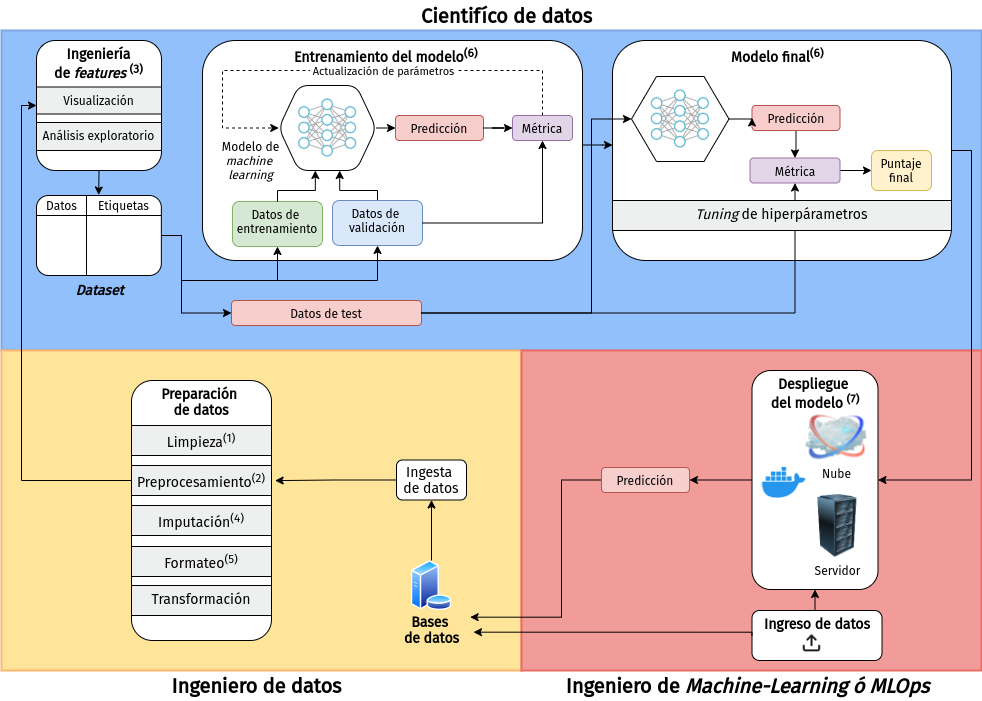
\includegraphics[width=1\textwidth]{ml-cycle.png}
		\caption{Arquitectura de un sistema de inteligencia artificial.}
		\label{fig:flowchartml.}
	\end{center}
\end{figure}

%No obstante para exponer el desarrollo de cada una de estas etapas es imprescindible elaborar un marco teórico que nos brinde contexto y herramientas para afrontar el problema a resolver.

\clearpage

\subsection{Objetivos}
\subsubsection{Objetivos principales}
Crear un modelo de \textit{Machine Learning} cuyo fin será el pronóstico de la cantidad de defectos graves de las unidades en la línea de producción de una planta automotriz.

\subsubsection{Objetivos secundarios}

\begin{itemize}
	\item Evaluar los diversos algoritmos disponibles de \textit{Machine Learning}, explorando todas las posibilidades en aras de identificar el modelo que mejor se adapte al problema a afrontar.
	      	      	      	
	\item Analizar los principios fundamentales de las redes neuronales \textit{feedforward}, convolucionales y recurrentes, así como sus elementos, algoritmos y arquitecturas que posibilitan su funcionalidad. Explorar y reconocer fortalezas y debilidades de cada uno según el tipo de problema a afrontar.
	      	      	      	
	\item Establecer y evaluar la mejor configuración de parámetros para una determinada arquitectura de red con el fin de optimizar su desempeño.
	      	      	      	
	\item Identificar, describir y clasificar las series temporales para evaluar su aplicación en la solución.
	      	      	      	
	\item Analizar la entropía de la serie de datos para determinar si es posible establecer una correlación.
	      	      	      	
	\item Examinar el problema a afrontar en su contexto, para así determinar los requerimientos del mismo. Posteriormente haciendo uso de las herramientas para manipulación de datos obtener un formato acorde de la serie temporal para alimentar los modelos.
	      	      	      	
\end{itemize}

\clearpage

\subsection{Requerimientos}
En ingeniería, los requerimientos se utilizan como datos de entrada en la etapa del diseño del producto. Establecen qué debe hacer el sistema, aunque no especifican la manera en que debe hacerlo. \citep{sommerville2015software}

Existen dos tipos de requerimientos:
\begin{itemize}[noitemsep, topsep=2pt]
	\item \textbf{Funcionales}: son enunciados acerca de servicios que el sistema debe brindar, su reacción a entradas particulares y comportamiento en situaciones particulares.
	\item \textbf{No funcionales}: no se refieren directamente a la funcionalidad del sistema sino a las propiedades que emergen de ella como la fiabilidad, la capacidad de almacenamiento, disponibilidad, etc. Suelen aplicarse al sistema como un todo, más que a características específicas del sistema.
\end{itemize}

\vspace{0.3cm}

Para especificar estos requerimientos se ejecutaron las siguientes etapas:
\begin{itemize}[topsep=2pt]
	\item \textbf{Entrevista}:  Se realizó una entrevista con el responsable del departamento Calidad Fabricación en la cuál se planteó la posibilidad de crear este sistema dado el potencial de los datos recabados por la usina. Esta propuesta fue aceptada y se elevó a los superiores para su aprobación debido a materia de confidencialidad.
	\item \textbf{Investigación del estado del arte}: Se profundizó en el conocimiento sobre las herramientas del campo de la ciencia de datos y \textit{machine-learning}. Esto incluyó el perfeccionamiento del uso de las librerías e investigación sobre algoritmos y modelos de inteligencia artificial, lo que permitió obtener una mejor perspectiva sobre el sistema a desarrollar al conocer las posibilidades y limitaciones del área.
	\item \textbf{Entrevista cerrada}: Se repitió la primer etapa pero teniendo en cuenta la información recabada en la etapa anterior. Se transmitió el conocimiento adquirido al responsable para alinear los objetivos propuestos, añadiendo nuevas consideraciones y descartando funcionalidades inviables.
\end{itemize}

\subsubsection{Requerimientos funcionales}
Los requerimientos del sistema han sido obtenidos en base al estudio teórico de los sistemas disponibles para lograr nuestro objetivo. Los mismos son presentados en el Cuadro~\ref{tab:functional-requirements}.

\begin{table}[H]
	\centering
	\begin{tabular}{p{0.07\linewidth} p{0.87\linewidth}}
		\hline
		\multicolumn{1}{c}{\textbf{ID}} & \multicolumn{1}{c}{\textbf{Descripción}}                                                                 \\ \hline
		RF1                             & El sistema deber tomar los datos desde las bases de datos de la compañía.                               \\
		RF2                             & El \textit{pipeline} de datos debe procesar los datos para entregarlos al modelo en un formato acorde.    \\
		RF3                             & El \textit{pipeline} de datos debe tolerar fallos en la entrada de datos soportando formatos imprevistos. \\
		RF4                             & El modelo debe guardar todas sus inferencias en la base de datos para revisión de rendimiento.           \\
		RF5                             & El modelo debe recibir y entregar un flujo continuo de datos en tiempo real.                              \\
		RF6                             & El sistema debe permitir un reporte que se crea dentro del \textit{pipeline}.                             \\
		RF7                             & El sistema debe proveer una API para ser consumida desde una página web.                                 \\ \hline
	\end{tabular}
	\caption{Requerimientos funcionales.}
	\label{tab:functional-requirements}
\end{table}

\subsubsection{Requerimientos no funcionales}
Estos fueron especificados en conjunto con el director del Proyecto Integrador y acordados en la entrevista final con el responsable de la fábrica.

\begin{table}[H]
	\centering
	\begin{tabular}{p{0.07\linewidth} p{0.87\linewidth}}
		\hline
		\multicolumn{1}{c}{\textbf{ID}} & \multicolumn{1}{c}{\textbf{Descripción}}                                                                                         \\ \hline
		RNF1                            & Optimizar el tiempo de respuesta del \textit{pipeline} para evitar cuello de botella.                                             \\
		RNF2                            & Diseñar pruebas para corroborar fiabilidad del sistema.                                                                          \\
		RNF3                            & El sistema será desarrollado enteramente en un lenguaje que facilite la integración entre los diversos componentes del sistema. \\
		RNF4                            & El modelo deberá lograr un rendimiento satisfactorio mínimo (65\%$\leq$precisión).                                             \\
		RNF5                            & El sistema debe ser accesible para cualquier usuario en la fábrica que lo necesite.                                              \\
		RNF6                            & El sistema utilizará un \textit{framework} de \textit{machine-learning} con respaldo de la comunidad para obtener soporte.       \\
		RNF7                            & El sistema debe proveer una API para ser consumida desde una página web.                                                         \\ \hline
	\end{tabular}
	\caption{Requerimientos no funcionales.}
	\label{tab:non-functional-requirements}
\end{table}

\subsection{Riesgos}
Un riesgo se define como un evento o condición incierta que en caso de ocurrir tendrá consecuencia sobre al menos uno de los requerimientos del proyecto.
\subsubsection{Tipos de riesgos} \label{sec:risk-types}
Se pueden identificar varios tipos de riesgos en un sistema como el que se intenta desarrollar.
\begin{itemize}[noitemsep, topsep=2pt]
	\item \textbf{Riesgos de proyecto} (P): amenazan la planificación del proyecto, principalmente los aspectos relacionados al tiempo.
	\item \textbf{Riesgos técnicos} (T): repercuten directamente en la calidad del producto.
	\item \textbf{Riesgos de negocio} (N): comprometen la viabilidad del proyecto.
\end{itemize}

\subsection{Gestión de riesgos}
Es un enfoque estructurado para \textit{manejar} la incertidumbre ante amenazas a través de una secuencia de actividades que tienen como objetivo reducir los efectos negativos de los riesgos ya sea evadiendolos si es posible o aceptando las consecuencias en el peor de los casos. 

Las etapas que lo componen son las siguientes:
\begin{enumerate}[noitemsep, topsep=2pt]
	\item \textbf{Identificación de riesgos}.
	\item \textbf{Análisis de riesgos}.
	\item \textbf{Selección de riesgos}.
	\item \textbf{Elaboración de planes de riesgos}.
\end{enumerate}

\subsubsection{Identificación de los riesgos}
Se realizó en base al conocimiento existente sobre los datos y el modelo a desarrollar. Los riesgos fueron clasificados según lo visto en la sección~\ref{sec:risk-types}.

\begin{table}[H]
	\centering
	\begin{tabular}{p{0.3\linewidth} p{0.63\linewidth}}
		\hline
		\multicolumn{1}{c}{\textbf{Riesgo}}            &   
		\multicolumn{1}{c}{\textbf{Descripción}} \\ \hline
		Aumento del tiempo de desarrollo del proyecto. &   
		Que el producto a realizar sea de mayor magnitud a la estimada, llevando a mayores tiempos de desarrollo. \\
		Planificación optimista.                      &   
		Se planifica el proyecto en base a criterios de situaciones óptimas o ideales en las que no se presentan problemas graves. \\ \hline
	\end{tabular}
	\caption{Identificación de riesgos de proyecto.}
	\label{tab:project-risks}
\end{table}

\begin{table}[H]
	\centering
	\begin{tabular}{p{0.3\linewidth} p{0.63\linewidth}}
		\hline
		\multicolumn{1}{c}{\textbf{Riesgo}}                             &   
		\multicolumn{1}{c}{\textbf{Descripción}} \\ \hline
		Desestimación de inversión.                                   &   
		La compañía una vez que el desarrollo del producto se encuentre en etapa avanzada hará un análisis de costes y beneficios para decidir la culminación total del proyecto. \\
		Falta de personal técnico para conformar equipo de desarrollo. &   
		La compañía debe evaluar el despliegue técnico que necesita el modelo ya que la naturaleza de este es transversal a varios sistemas de la fábrica y su implementación requiere de un equipo de desarrollo especializado. \\ \hline
	\end{tabular}
	\caption{Identificación de riesgos de negocio.}
	\label{tab:business-risks}
\end{table}

\begin{table}[H]
	\centering
	\begin{tabular}{p{0.3\linewidth} p{0.63\linewidth}}
		\hline
		\multicolumn{1}{c}{\textbf{Riesgo}}                                                                                  &   
		\multicolumn{1}{c}{\textbf{Descripción}} \\ \hline
		Arquitectura de sistemas de la organización no apta para el despliegue del modelo.                                  &   
		Muchos de los sistemas utilizados en la organización datan de largo tiempo e inclusive no reciben mantenimiento activo. Por tanto es necesario revisar la factibilidad de la integración del producto con estos sistemas y la obtención de los datos necesarios. \\
		Servidor con \textit{hardware} insuficiente para ejecutar el modelo.                                                 &   
		La compañía deberá evaluar la adquisición o alquiler de \textit{hardware} especifico y necesario para el entrenamiento e inferencia del modelo. \\
		Incapacidad de acceso en tiempo real a las bases de datos. &   
		Se deben actualizar las bases de datos actuales (actualmente bajo el modelo SAP) para proveer los datos al modelo en tiempo real para su inferencia. \\
		Pérdida del modelo entrenado por situación imprevista                                                              &   
		En ciertas ocasiones los modelos son entrenados por largos intervalos de tiempo para luego obtener los reportes y sus pesos. Sin embargo a veces surgen situaciones imprevistas que corrompen el código con el tiempo de ejecución avanzado provocando la pérdida de estos datos. \\ \hline
	\end{tabular}
	\caption{Identificación de riesgos técnicos.}
	\label{tab:technical-risks}
\end{table}

\clearpage

\subsubsection{Análisis de riesgos}
No es posible tratar todos los riesgos existentes por tanto se procederá a cuantificar los mismos para compararlos y priorizar aquellos que se consideren con mayor relevancia para su tratamiento. 

La posibilidad de ocurrencia se medirá de forma continua entre 0 y 1, donde 0 significa que es prácticamente imposible que ocurra y 1 es muy probable. Por otro lado, el impacto se medirá en una escala discreta entre 1 y 4 cuyos niveles representan:
\begin{enumerate}[noitemsep, topsep=2pt]
	\item Insignificante.
	\item Tolerable.
	\item Importante.
	\item Muy grave.
\end{enumerate}

La exposición $(E)$ es el producto entre la probabilidad $(P)$ y el impacto del riesgo $(R)$, representando con este valor la gravedad del mismo.

$$ E = PI $$

\begin{table}[H]
	\centering
	\begin{tabular}{p{0.67\linewidth} c c c c}
		\hline
		\multicolumn{1}{c}{\textbf{Riesgos}} &
		\multicolumn{1}{c}{\textbf{Tipo}} &
		\multicolumn{1}{c}{\textbf{P}} &
		\multicolumn{1}{c}{\textbf{I}} &
		\multicolumn{1}{c}{\textbf{E}} \\ \hline
		Aumento de la complejidad del proyecto.                         & P & 0,4 & 2 & 0,8 \\
		Planificación optimista.                                       & P & 0,5 & 3 & 1,5 \\
		Desestimación de inversión.                                   & N & 0,8 & 3 & 2,4 \\
		Falta de personal técnico para conformar equipo de desarrollo. & N & 0,6 & 3 & 1,8 \\
		Arquitectura de sistemas de la organización no apta para el despliegue del modelo. &
		T &
		0,9 &
		3 &
		\textbf{2,7} \\
		Servidor con hardware insuficiente para ejecutar el modelo.     & T & 0,7 & 3 & 2,1 \\
		Se debe acceder a las bases de datos a través de un protocolo que permite la transferencia de datos en tiempo real. &
		T &
		0,7 &
		4 &
		\textbf{2,8} \\
		Pérdida del modelo entrenado por situación imprevista         & T & 0,6 & 2 & 1,2 \\ \hline
	\end{tabular}
	\caption{Riesgos.}
	\label{tab:risk-table}
\end{table}

\clearpage

\subsubsection{Selección de riesgos}
Para esta tarea se decidió utilizar el principio de Pareto \citep{pareto}, el cual establece que de forma general, el 20\% del esfuerzo produce el 80\% de los resultados. O dicho de otra manera: el 80\% de las consecuencias provienen del 20\% de las causas, así  le daremos prioridad al conjunto de riesgos de mayor exposición para mitigar sus efectos. El 20\% de los 8 riesgos mostrados en el cuadro~\ref{tab:risk-table} es 1.6, el cual redondearemos a 2.

\subsubsection{Elaboración de planes de riesgos}
Para esta tarea realizaremos dos tipos de planes.
\begin{itemize}[noitemsep]
	\item \textbf{Plan de mitigación}: su objetivo es reducir la probabilidad de ocurrencia del riesgo o el impacto que el mismo puede provocar.
	\item \textbf{Plan de contingencia}: está comprendido por acciones que se deberán realizar solamente si el riesgo se presenta.	
\end{itemize}

Los dos riesgos principales son de tipo técnico, esto en gran parte se debe a la escasa actualización de los sistemas de la empresa. Esto provoca un gran déficit tecnológico que vulnera las oportunidades de soluciones informáticas en diversas áreas de la fábrica. No obstante, en el cuadro~\ref{tab:risks-plans} definimos planes de mitigación y contingencia para cada uno de estos riesgos.

\begin{table}[H]
\centering
\begin{tabular}{p{0.2\linewidth} p{0.35\linewidth} p{0.35\linewidth}}
\hline
\multicolumn{1}{c}{\textbf{Riesgo}} &
  \multicolumn{1}{c}{\textbf{Plan de mitigación}} &
  \multicolumn{1}{c}{\textbf{Plan de contingencia}} \\ \hline
Arquitectura de sistemas de la organización no apta para el despliegue del modelo. &
  Contactarse desde una etapa temprana con el departamento de informática de la empresa para determinar el estado actual de los sistemas. En caso que sea realizable la implementación podemos trabajar desde etapas tempranas teniendo en cuenta los sistemas, de este modo se ahorran tiempos al momento de la integración. &
  Realizar un reporte detallado de costos y beneficios del proyecto para que los directivos analicen de forma más organizada la información para tomar la decisión. Esto incluiría diversos beneficios como la actualización de varios sistemas de la fábrica que no reciben soporte ya y por tanto tienen un rendimiento reducido además de presentar vulnerabilidades. \\
Incapacidad de acceso en tiempo real a las bases de datos. &
  Comunicarse con el departamento de informática con el objetivo de obtener soporte oficial de la empresa creadora del sistema de base de datos. La idea es explorar la posibilidad de crear un protocolo que permita conectar nuestro sistema con la base de datos en tiempo real. &
  Proponer la migración o duplicación de los datos necesarios a una base de datos relacional que permita realizar consultas en tiempo real. \\ \hline
\end{tabular}
\caption{Elaboración de planes de riesgo.}
\label{tab:risks-plans}
\end{table}

\clearpage

\section{Clasificación de modelos de inteligencia artificial}

Hagamos algunas definiciones para ponernos en contexto del campo sobre el cual este proyecto integrador será desarrollado.

\subsection{Inteligencia Artificial}

\begin{quote}
	La \textit{Inteligencia Artificial (Artificial Intelligence)} se define como el estudio de los "agentes inteligentes", i.e. cualquier dispositivo que perciba su entorno y tome medidas que maximicen sus posibilidades de lograr con éxito sus objetivos.
			  
	\hfill \citet{poole1998}
\end{quote}

Esta definición nos da la idea de que la IA es un sistema reactivo, que reacciona a cambios externos y actúa en consecuencia.

\subsubsection{Aprendizaje automático} \label{machinelearning}

\begin{quote}
	El \textit{aprendizaje automático (Machine Learning)} es el estudio científico de algoritmos y modelos estadísticos que los sistemas informáticos utilizan para realizar una tarea específica sin utilizar instrucciones explícitas, sino que se basan en patrones e inferencia. Es visto como un subcampo de inteligencia artificial. Los algoritmos de aprendizaje automático crean un modelo matemático basado en datos de muestra, conocidos como "datos de entrenamiento", para hacer predicciones o decisiones sin ser programado explícitamente para realizar la tarea.
			  
	\hfill \citet{bishop2006pattern}
\end{quote}

Por tanto el Aprendizaje Automático es la generación de un modelo de predicción de salida a partir de grandes cantidades de datos de entrada, realizando un tratamiento de los mismos a través de varias etapas. Es importante destacar la independencia del aprendizaje automático al momento de tomar decisiones a partir de los datos proporcionados sin intervención externa, es decir que no hay una especificación de reglas que dictan cómo deben ser tomadas estas decisiones.

A su vez, los modelos obtenidos a partir de los algoritmos de \textit{Machine Learning} deben tener la capacidad de predecir a partir de nuevos datos, nunca antes procesados por el modelo, a esto se lo conoce como \textbf{generalización}. 

\subsection{Preprocesamiento} \label{preprocessing}
Este punto es vital para cualquier proyecto que utiliza algoritmos de \textit{Machine Learning}, debido a que los datos incluidos en los conjuntos conocidos como \textit{datasets}, no suelen presentarse en condiciones para obtener el óptimo rendimiento de los algoritmos de aprendizaje. Estos datos suelen estar desbalanceados, con faltantes o ruidosos, entre otras cuestiones. 

Una vez obtenido el \textit{dataset} de entrada es primordial investigar, limpiar y transformar los datos con diversas técnicas. Una vez que los datos estén en condiciones procedemos al entrenamiento de nuestro modelo, con el propósito de lograr un desempeño óptimo.

Para lograr este objetivo se aplican técnicas tales como normalización, reescalado, reducción de dimensionalidad, discretización, tratamiento de anomalías y \textit{outliers}.

\subsection{Aprendizaje supervisado} \label{supervised}
El aprendizaje supervisado es el enfoque más utilizado y comprendido para el aprendizaje automático, siendo ideal para tareas donde el modelo necesita predecir resultados. Implica una entrada y salida para cada pieza de datos en su \textit{dataset}. Por ejemplo, una entrada podría ser una imagen y la salida podría ser la respuesta a ``?`es esto un gato?''.

Cada una de estas piezas de datos que alimentan el modelo se denominan \textit{features} (características), que son esencialmente una propiedad individual medible como puede ser la edad o el peso de una persona.

En el aprendizaje supervisado siempre hay una distinción entre el conjunto de entrenamiento o \textit{training} para el cual se nos proporciona la etiqueta (o \textit{label}), y el conjunto de prueba para el cual la etiqueta debe ser inferida. 

El algoritmo de aprendizaje debe ajustar el modelo predictivo al \textit{dataset} de entrenamiento y usamos el \textit{dataset} de prueba para evaluar la capacidad de generalización. El aprendizaje supervisado es ideal para tareas donde el modelo necesita predecir resultados.

Estos problemas de predicción podrían involucrar el uso de estadísticas para predecir un valor (por ejemplo, $20 kg$, $\$1498$, $0.80 cm$) o categorizar datos basados en clasificaciones dadas (por ejemplo, ``gato'', ``verde'', ``feliz'') \cite{norman2019aprendizaje}. El siguiente paso es profundizar en las dos categorías de aprendizaje supervisado que existen: clasificación y regresión.

\subsubsection{Clasificación}

En clasificación, la etiqueta es discreta y se intenta categorizar el elemento. Por tanto, se proporciona una distinción clara entre categorías y se denominan variables categóricas.

\textbf{Clasificación de variables categóricas según tipo}: 
\begin{itemize}[noitemsep, topsep=2pt]
	\item \textbf{Ordinales}: tienen asociado un orden. \textit{e.g.} las tallas de las camisetas ``$XL > L > M > S$''.
	\item \textbf{Nominales}: no implican un orden.\textit{e.g.} no podemos asumir (en general) ``$naranja > azul > verde$''
\end{itemize}

\textbf{Tipo de clasificación según cantidad de variables}:
\begin{itemize}[noitemsep, topsep=2pt]
	\item \textbf{Binaria}: se elige entre dos categorías, \textit{e.g.} clasificar un mail entre \texttt{Spam} y \texttt{No Spam}.
	\item \textbf{Multiclase}: se elige entre más de dos categorías, \textit{e.g.} clasificar un conjunto de imágenes de frutas, donde habrá manzanas, naranjas y peras. 
\end{itemize} 

Para poder apreciar el concepto de clasificación binaria, en la Fig.~\ref{fig:binaryclassification.}  \cite{GitHubpa25:online} se han graficado datos bidimensionales, es decir que cada dato tiene dos valores asociados de acuerdo a los ejes X e Y. El dataset cuenta con 100 muestras, las cuales están divididas en dos clases: ceros (círculos azules) y unos (cuadrados rojos). 

\begin{figure}[H]
	\begin{center}				
		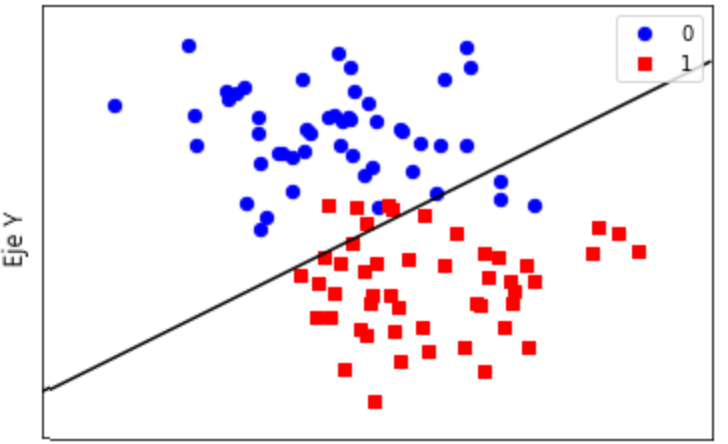
\includegraphics[width=0.5\textwidth]{tesis_2.png}
		\caption{Ejemplo de clasificación binaria.}
		\label{fig:binaryclassification.}
	\end{center}
\end{figure}

El modelo a utilizar para la predicción será uno de los más conocidos y simples de utilizar en clasificación, \textbf{regresión logística}. Éste es un modelo lineal, lo que significa que creará una frontera de decisión que es lineal en el espacio de entrada, en 2D esto quiere decir que generará una línea recta para separar los puntos azules de los rojos.

Como puede observarse, el modelo no es 100\% preciso ya que algunos puntos azules están en la categoría de los rojos y viceversa, por eso es que existen diversos modelos y debemos elegir según nuestro criterio cuál de ellos se adecúa mejor a nuestras necesidades.

Debido a la cantidad de diversos algoritmos que existen para clasificación es posible caracterizarlos en función de sus pros y contras como se observa en el Cuadro 1.

\subsubsection{Regresión}

En regresión, la etiqueta es continua, es decir una salida real. Podríamos querer estimar la edad de un objeto basándonos en su imagen: esto sería regresión, porque la etiqueta (edad) es una cantidad continua \citep{GitHubpa25:online}.

En los problemas de regresión, tenemos como entradas las \textbf{variables independientes o explicativas} y las salidas o etiquetas son \textbf{variables continuas}. Por lo tanto, los modelos de regresión deben encontrar una relación (función lineal, polinomial, entre otras) que nos permitan predecir la salida.

\begin{figure}[H]
	\begin{center}				
		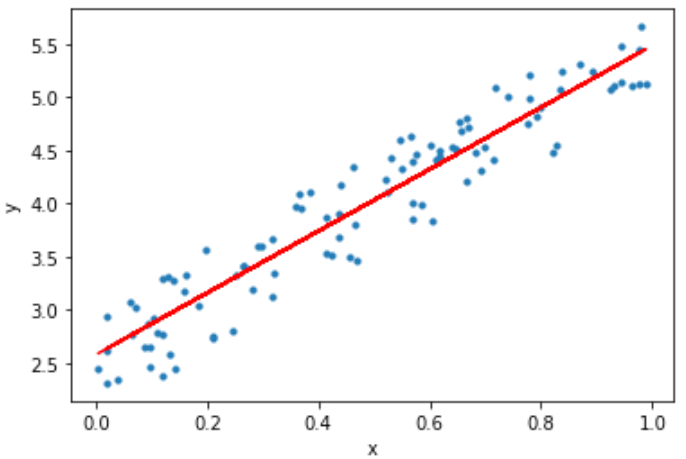
\includegraphics[width=0.5\textwidth]{tesis_9.png}
		\caption{Ejemplo de regresión lineal.}
		\label{fig:regressionlinear.}
	\end{center}
\end{figure}

Para poder apreciar el concepto de regresión lineal, en la Fig.~\ref{fig:regressionlinear.} se tienen 100 muestras con sus respectivas etiquetas, entonces lo que hace el algoritmo de regresión lineal es ajustar una línea recta que minimice la distancia (en este caso distancia euclídea) entre los puntos de la muestra y dicha recta. Al obtener la recta, disponemos de los parámetros del modelo como son los coeficientes y la intersección, por ende estamos en condiciones de predecir la salida de nuevas muestras.

Así como pudimos listar las ventajas y desventajas con los distintos algoritmos de clasificación también es aplicable a los de regresión como vemos en el Cuadro 2.


\includepdf[pages={12}]{anexo.pdf}


\includepdf[pages={13}]{anexo.pdf}

\subsection{Selección de algoritmo en base al \textit{dataset}}
En la Fig.~\ref{fig:maindiagram.} obtenemos una vista general sobre que hacer con nuestros datos en función a nuestro objetivo.

\begin{figure}[H]
	\begin{center}
		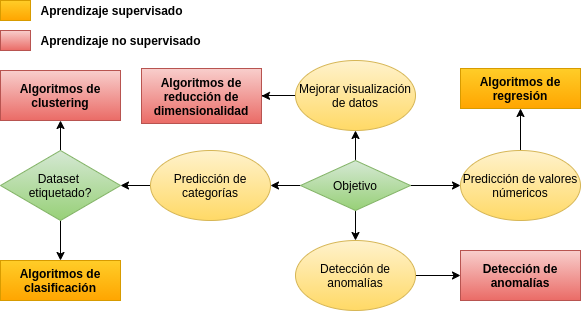
\includegraphics[width=0.75\textwidth]{maindiagram.png}
		\caption{Diagrama general de algoritmos de aprendizaje supervisado y no supervisado.}
		\label{fig:maindiagram.}
	\end{center}
\end{figure}

\subsubsection{Algoritmos supervisados}
\begin{figure}[H]
	\begin{center}
		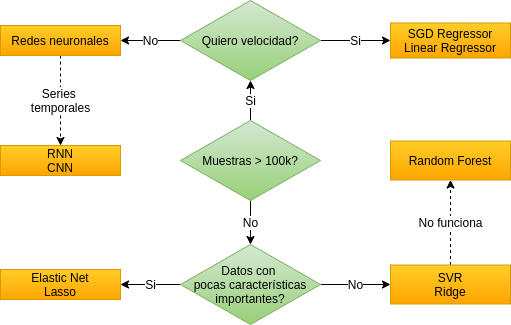
\includegraphics[width=0.75\textwidth]{regressiondiagram.png}
		\caption{Diagrama general de los algoritmos de regresión.}
		\label{fig:regressiondiagram.}
	\end{center}
\end{figure}

\begin{figure}[H]
	\begin{center}				
		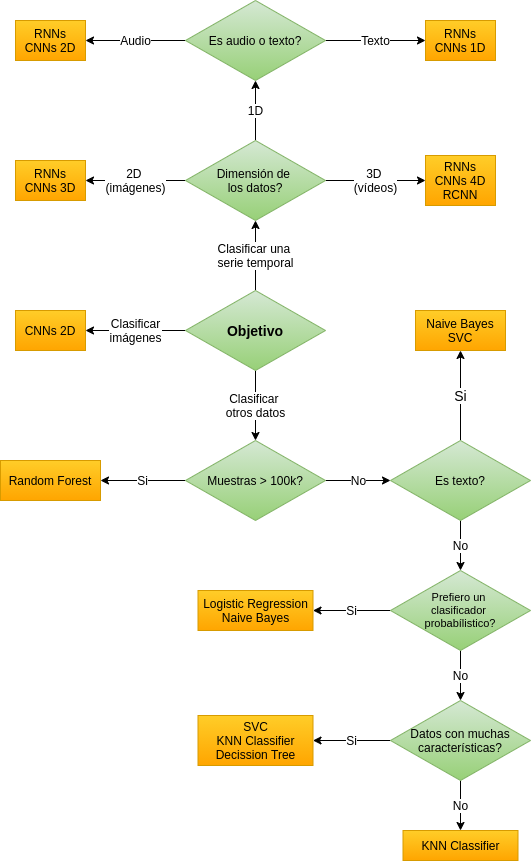
\includegraphics[width=0.9\textwidth]{classificationdiagram.png}
		\caption{Diagrama general de los algoritmos de clasificación.}
		\label{fig:classificationdiagram.}
	\end{center}
\end{figure}

\subsubsection{Algoritmos no supervisados}

\begin{figure}[H]
	\begin{center}				
		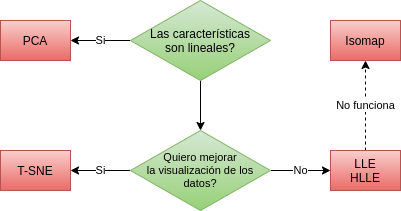
\includegraphics[width=0.65\textwidth]{dimreduxdiagram.png}
		\caption{Diagrama general de los algoritmos de reducción de dimensión.}
		\label{fig:dimreduxdiagram.}
	\end{center}
\end{figure}

\begin{figure}[H]
	\begin{center}				
		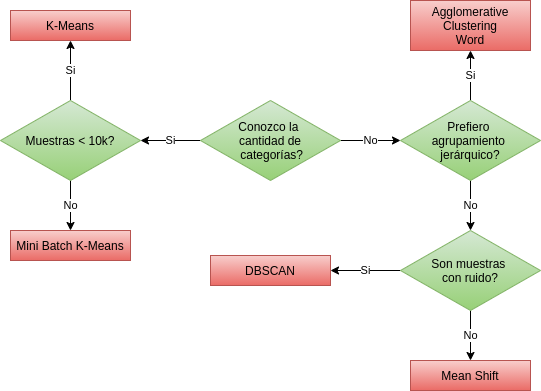
\includegraphics[width=0.75\textwidth]{clusteringdiagram.png}
		\caption{Diagrama general de los algoritmos de \textit{clustering}.}
		\label{fig:clusteringdiagram.}
	\end{center}
\end{figure}

\begin{figure}[H]
	\begin{center}				
		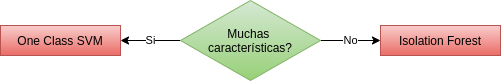
\includegraphics[width=0.75\textwidth]{anomalydiagram.png}
		\caption{Diagrama general de los algoritmos de detección de anomalías.}
		\label{fig:anomalydiagram.}
	\end{center}
\end{figure}

\clearpage

\section{Redes neuronales}
La palabra neuronal es la forma adjetiva de "neurona", y red denota una estructura tipo grafo; por lo tanto, una \textit{Red Neuronal Artificial} es un sistema de computación que intenta imitar (o al menos, está inspirado en) las conexiones neuronales en nuestro sistema nervioso. Las redes neuronales artificiales también se denominan \textit{redes neuronales} o \textit{sistemas neuronales artificiales}. Es común abreviar la red neuronal artificial y referirse a ellas como "NN". \citep{rosebrock2017deep}

Para que un sistema se considere un NN, debe contener una estructura de grafo dirigida y etiquetada donde cada nodo del gráfico realice un cálculo simple. Según la teoría de grafos, sabemos que un gráfico dirigido consiste en un conjunto de nodos (es decir, vértices) y un conjunto de conexiones (es decir, bordes) que unen pares de nodos.

\begin{itemize}[noitemsep, topsep=2pt]
	\item Las entradas ingresan a la red. 
	\item Cada conexión lleva una señal a través de las dos capas ocultas en la red. 
	\item Una función final calcula la etiqueta de clase de salida.
\end{itemize}

\begin{figure}[H]
	\begin{center}				
		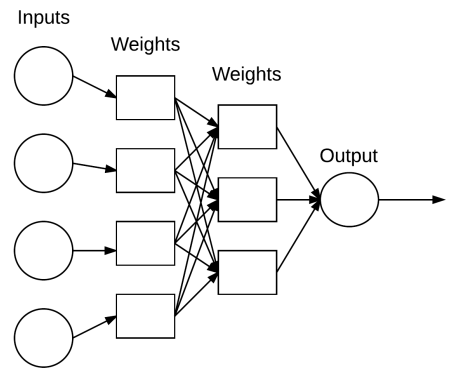
\includegraphics[width=0.6\textwidth]{018.png}
		\caption{Arquitectura simple de red neuronal. \cite{matich}}
		\label{fig:nn}
	\end{center}
\end{figure}

Cada nodo realiza un cálculo simple. Cada conexión transporta una señal (es decir, la salida del cálculo) de un nodo a otro, marcada por un peso que indica el grado en que la señal se amplifica o disminuye. Algunas conexiones tienen grandes pesos positivos que amplifican la señal, lo que indica que la señal es muy importante al hacer una clasificación. 

\clearpage

Otros tienen pesos negativos, lo que disminuye la intensidad de la señal, lo que especifica que la salida del nodo es menos importante en la clasificación final. Llamamos a dicho sistema una Red Neuronal Artificial si consta de una estructura de grafo (como en la figura \ref{fig:nn}) con pesos de conexión que se pueden modificar utilizando un algoritmo de aprendizaje.

\subsection{Relación con la biología}
Nuestros cerebros están compuestos por aproximadamente 10 mil millones de neuronas, cada una conectada a otras 10000 neuronas. El cuerpo celular de la neurona se llama soma, donde las entradas (dendritas) y las salidas (axones) conectan el soma con otro (figura \ref{fig:realneuron}).

\begin{figure}[H]
	\begin{center}				
		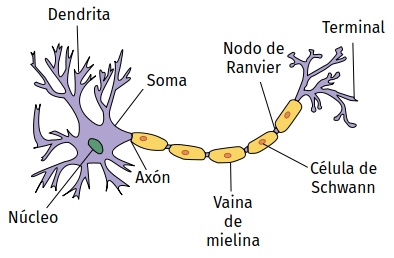
\includegraphics[width=0.5\textwidth]{019.png}
		\caption{Estructura de una neurona biológica. \citep{neurona_wiki}}
		\label{fig:realneuron}
	\end{center}
\end{figure}

Cada neurona recibe entradas electroquímicas de otras neuronas en sus dendritas. Si estas entradas eléctricas son lo suficientemente potentes como para activar la neurona, entonces la neurona activada transmite la señal a lo largo de su axón, transmitiéndola a las dendritas de otras neuronas. Estas neuronas unidas también pueden activarse, continuando así el proceso de transmitir el mensaje.
La conclusión clave aquí es que el disparo de una neurona es una operación binaria: la neurona se dispara o no se dispara. No hay diferentes "grados" de disparo. En pocas palabras, una neurona solo se disparará si la señal total recibida en el soma excede un umbral dado.
Sin embargo, tenga en cuenta que los ANN simplemente se inspiran en lo que sabemos sobre el cerebro y cómo funciona. El objetivo del aprendizaje profundo no es imitar cómo funcionan nuestros cerebros, sino tomar las piezas que entendemos y permitirnos trazar paralelos similares en nuestro propio trabajo.

\subsection{Modelos artificiales}
Comencemos por ver un NN básico que realiza una suma ponderada simple de las entradas o \textit{inputs} en la figura \ref{fig:simplenn}. Los valores $x_1$, $x_2$ y $x_3$ son las \textit{inputs} a nuestro NN y generalmente corresponden a una sola fila (es decir, punto de datos) de nuestra matriz de diseño. El valor constante 1 es nuestro sesgo o \textit{bias} que se supone incrustado en la matriz de diseño. Podemos pensar en estas \textit{inputs} como los vectores de características o \textit{features} de entrada a la NN.

\begin{figure}[H]
	\begin{center}				
		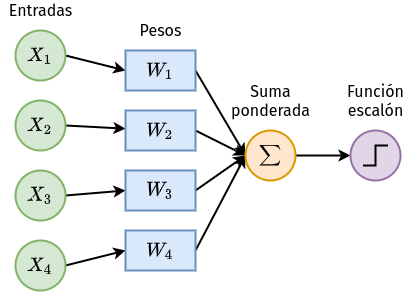
\includegraphics[width=0.6\textwidth]{020.png}
		\caption{Simple NN.}
		\label{fig:simplenn}
	\end{center}
\end{figure}

Cada $x$ está conectada a una neurona a través de un vector de peso $W$ que consiste en $w_1, w_2, \ldots w_n$, lo que significa que para cada entrada $x$ también tenemos un peso asociado $w$.
Finalmente, el nodo de salida a la derecha toma la suma ponderada, aplica una función de activación $f$ (utilizada para determinar si la neurona se "dispara" o no) y genera un valor. Expresando la salida matemáticamente, normalmente encontrarás las siguientes tres formas:
\begin{itemize}[noitemsep, topsep=2pt]
	\item $f(w_1x_1 + w_2x_2 + \cdots + w_nx_n)$
	\item $f(\sum_{i=1}^{n} w_ix_i)$	
	\item O $f(net)$, donde $net = \sum_{i=1}^{n} w_ix_i$
\end{itemize}

\subsection{Funciones de activación}
La función de activación más simple es la "función de paso", utilizada por el algoritmo Perceptron.

$
f(net) =
\left\{
\begin{array}{ll}
	1 & \mbox{si } net > 0    \\
	0 & \mbox{si } net \leq 0 
\end{array}
\right.
$

Esta es una función de umbral muy simple, sin embargo, aunque es fácil de usar e intuitiva, no es diferenciable, lo cual puede llevar a problemas cuando apliquemos el descenso por gradiente.
Por ello se presentan en la figura \ref{fig:typesfactivation} diferentes tipos de funciones de activación con sus respectivos gráficos.

\begin{figure}[H]
	\begin{center}				
		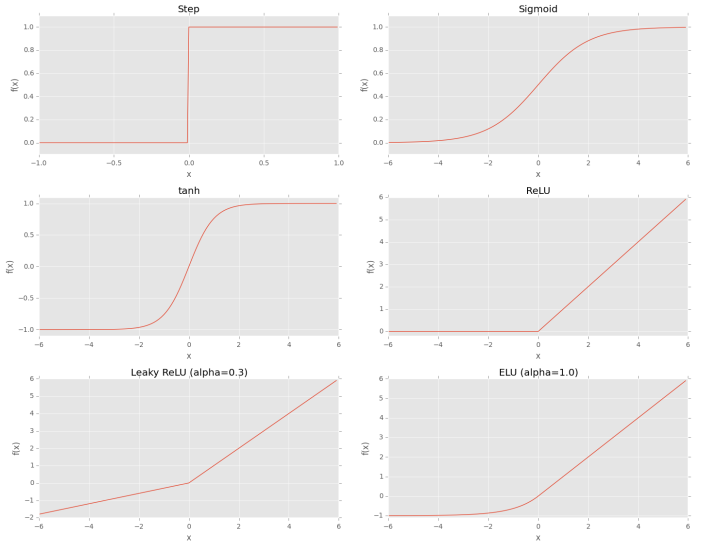
\includegraphics[width=1\textwidth]{021.png}
		\caption{\textbf{Arriba-izquierda}: Función escalón. \textbf{Arriba-derecha}: Función sigmoidea. \textbf{Medio-izquierda}: Tangente hiperbólica. \textbf{Medio-derecha}: activación ReLU (función activación más usada en \textit{Deep Learning}).
			\textbf{Abajo-izquierda}: Leaky ReLU, variante de ReLU que permite valores negativos. \textbf{Abajo-derecha}:
			Lineal, la primer función utilizada.\citep{AyyuceKizrak2020Jan}}
		\label{fig:typesfactivation}
	\end{center}
\end{figure}

\clearpage

Una de las funciones de activación más usadas en la historia de la literatura de NN es la función sigmoidea, que se define a continuación:

\begin{equation}
	t=\sum_{i=1}^{n}w_ix_i \quad s(t)=\frac{1}{1+e^{-t}}
\end{equation}

La función sigmoidea es una mejor opción para el aprendizaje que la función de paso simple, ya que:
\begin{enumerate}[noitemsep, topsep=2pt]
	\item Es continua y diferenciable en todas partes.
	\item Es simétrica alrededor del eje y.
	\item Se acerca asintóticamente a sus valores de saturación.
\end{enumerate}
La principal ventaja aquí es que la suavidad de la función sigmoidea hace que sea más fácil diseñar algoritmos de aprendizaje. Sin embargo, hay dos grandes problemas con la función sigmoidea:
\begin{enumerate}[noitemsep, topsep=2pt]
	\item Las salidas del sigmoidea no están centradas en cero.
	\item Las neuronas saturadas esencialmente eliminan el gradiente, ya que el delta del gradiente será extremadamente pequeño.
\end{enumerate}

La tangente hiperbólica, o $tanh$ (con una forma similar a la sigmoidea) también se usó fuertemente como una función de activación hasta fines de la década de 1990.
La ecuación para $tanh$ sigue:
\begin{equation}
	f(z) = tanh(z) = \frac{e^z - e^{-z}}{e^z + e^{-z}}
\end{equation}
La función tanh está centrada en cero, pero los gradientes aún se eliminan cuando las neuronas se saturan.
Ahora sabemos que hay mejores opciones para las funciones de activación que las funciones sigmoidea y tanh. Específicamente, la Unidad Lineal Rectificada (ReLU), definida como:
\begin{equation}
	f(x) = max(0, x)
\end{equation}
Las ReLU también se denominan "funciones de rampa" debido a cómo se ven cuando se trazan. La función es cero para entradas negativas pero luego aumenta linealmente para positivas valores. La función ReLU no es saturable y también es extremadamente  eficiente computacionalmente.
Empíricamente, la función de activación ReLU tiende a superar a las funciones sigmoidea y tanh en casi todas las aplicaciones. Sin embargo, surge un problema cuando tenemos un valor de cero: no se puede tomar el gradiente.

\clearpage

\subsection{Arquitecturas de redes \textit{feedforward}}

Si bien hay muchas, muchas arquitecturas NN diferentes, la arquitectura más común es la red hacía adelante o \textit{feedforward}, como se presenta en la figura \ref{fig:nnff}.

\begin{figure}[H]
	\begin{center}				
		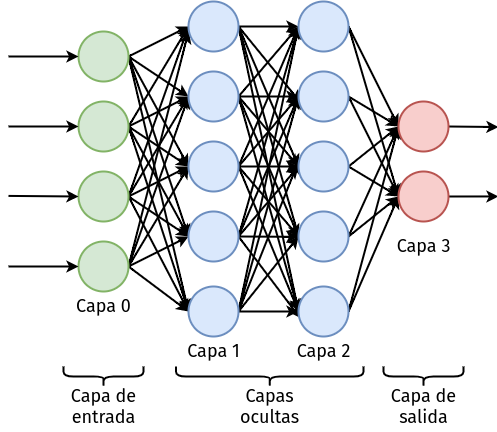
\includegraphics[width=0.65\textwidth]{022.png}
		\caption{Un ejemplo de una red neuronal \textit{feedforward}.}
		\label{fig:nnff}
	\end{center}
\end{figure}

En este tipo de arquitectura, solo se permite una conexión entre los nodos; de los nodos en la capa $i$ a los nodos en la capa $i + 1$ (de ahí el término \textit{feedforward}). No hay conexiones hacia atrás o entre capas permitidas. Cuando las redes de retroalimentación incluyen conexiones de retroalimentación (conexiones de salida que retroalimentan las entradas) se denominan redes neuronales recurrentes.

Para describir una red \textit{feedforward}, normalmente usamos una secuencia de enteros para depositar rápida y concisamente el número de nodos en cada capa. Por ejemplo, la red en la figura 10.5 anterior es una red de alimentación directa 3-2-3-2:

\begin{itemize}[noitemsep, topsep=2pt]
	\item La capa 0 contiene 3 entradas, nuestros valores $x_i$. Estos podrían ser intensidades de píxeles sin procesar de una imagen o un vector de características extraído de la imagen.
	\item Las capas 1 y 2 son capas ocultas que contienen 2 y 3 nodos, respectivamente.
	\item La capa 3 es la capa de salida o la capa visible: allí es donde obtenemos la clasificación de salida general de nuestra red. La capa de salida generalmente tiene tantos nodos como etiquetas de clase; un nodo para cada salida potencial.
\end{itemize}

\subsection{Redes multicapa}
Las redes multicapas, \textit{i.e.} con varias capas de neuronas pueden ser modeladas matemáticamente como se muestra a continuación.
Supongamos $W$ como la matriz de pesos y el vector $b$ como el vector sesgo o \textit{bias}.
Consideremos:
\begin{equation}
	z(x)=Wx+b=\sum_{i=1}^{n}w_ix_i+b
\end{equation}
Además cabe mencionar que la multiplicación punto a punto entre dos matrices de igual dimensión es lo que se conoce como el producto Hadamard.
\begin{equation}
	\sigma(z)=\frac{1}{1+e^{-z}}
\end{equation}
Por último definimos la salida de nuestro modelo como:
\begin{equation}
	\hat{y}=\sigma(\sum_{i=1}^{n}w_ix_i+b)
\end{equation}

\subsection{Función pérdida}

El objetivo del algoritmo de descenso de gradiente es minimizar la función de costo para que nuestro modelo neuronal pueda aprender.
Pero antes debemos definir que es la función costo o pérdida \cite{sgd}.
En el cálculo, los máximos (o mínimos) de cualquier función pueden ser descubiertos por:
\begin{enumerate}[noitemsep, topsep=2pt]
	\item Tomando la derivada de primer orden de la función e igualándola a 0. El punto encontrado de esta manera puede ser el punto de máximo o mínimo.
	\item Sustituimos estos valores (el punto que acabamos de encontrar) en la derivada de segundo orden de la función y pueden suceder 3 cosas:
	      \begin{itemize}
	      	\item si el valor es positivo, entonces el punto $s$ representa un mínimo local.
	      	\item si el valor sea negativo entonces $s$ representa un máximo local.
	      	\item si el valor es $0$ entonces $s$ es un punto de inflexión.
	      \end{itemize}
\end{enumerate}

Necesitamos cerrar la brecha entre la salida del modelo y la salida real. Cuanto menor sea la brecha, mejor será nuestro modelo en sus predicciones y más confianza mostrará al predecir.

La \textbf{función de pérdida o costo} esencialmente modela la diferencia entre la predicción de nuestro modelo y la salida real. Idealmente, si estos dos valores están muy separados, el valor de pérdida o el valor de error deberían ser mayores. Del mismo modo, si estos dos valores están más cerca, el valor del error debería ser bajo.
Una posible función de pérdida podría ser:
\begin{equation}
	J(\Theta)=\hat{y}-y / y\in\{0,1\}
\end{equation}
Pero, en lugar de tomar esta función como nuestra función de pérdida, terminamos considerando la siguiente función:
\begin{equation}
	J(\Theta)=\frac{\|\hat{y}-y\|^2}{2}
\end{equation}
Esta función se conoce como error al cuadrado . Simplemente tomamos la diferencia entre la salida real $y$ y la salida predicha $\hat{y}$ elevamos al cuadrado ese valor (de ahí el nombre) y lo dividimos entre 2.

Una de las principales razones para preferir el error al cuadrado en lugar del error absoluto es que el error al cuadrado es diferenciable en todas partes mientras que el error absoluto no lo es (su derivada no está definida en 0).

Además, los beneficios de la cuadratura incluyen:
\begin{itemize}[noitemsep, topsep=2pt]
	\item La cuadratura siempre da un valor positivo, por lo que la suma no será cero.
	\item Hablamos de suma aquí porque sumaremos los valores de pérdida o error para cada ítem en nuestro conjunto de datos de entrenamiento y luego haremos un promedio para encontrar la pérdida para todo el lote de ejemplos de entrenamiento.
	\item La cuadratura enfatiza las diferencias más grandes, una característica que resulta ser buena y mala.
\end{itemize}

La función de error que usaremos aquí se conoce como el error cuadrático medio y la fórmula es la siguiente:

\begin{equation}
	J(\Theta)=\frac{1}{2m} \sum_{i=1}^{m} (\hat{y_i}-y_i)^2
	\label{funcperdida}
\end{equation}

Calculamos el error al cuadrado para cada \textit{feature} en nuestro \textit{dataset} y luego encontramos el promedio de estos valores y esto representa el error general del modelo en nuestro conjunto de entrenamiento.

Consideremos el ejemplo de un solo ítem con 2 características, lo que significa que tenemos 2 valores de peso correspondientes y un valor de sesgo. En total, tenemos 3 parámetros para nuestro modelo.

\begin{equation}
	\hat{y} = w_1x_1 + w_2x_2 + b
\end{equation}

\begin{equation}
	J(\Theta)=\frac{1}{2m} \sum_{i=1}^{m} (w_1x_1^{(i)}+w_2x_2^{(i)}+b-y^{(i)})^2
\end{equation}

Queremos encontrar valores para nuestros pesos y el sesgo que minimiza el valor de nuestra función de pérdida. Dado que esta es una ecuación de múltiples variables, eso significa que tendríamos que tratar con derivadas parciales de la función de pérdida correspondiente a cada una de nuestras variables $w_1$, $w_2$ y $b$.

\begin{equation}
	\frac{\partial J}{\partial w_1} \frac{\partial J}{\partial w_2}
	\frac{\partial J}{\partial b}
\end{equation}

Esto puede parecer lo suficientemente simple porque solo tenemos 3 variables diferentes.
Sin embargo tenemos tantos pesos como features \textit{i.e.} $w_n$ pesos.

Hacer una optimización multivariable con tantas variables es computacionalmente ineficiente y no es manejable. Por lo tanto, recurrimos a alternativas y aproximaciones.

\subsection{Descenso de gradiente}

Es la capacidad de aprendizaje que otorga el algoritmo de descenso de gradiente lo que hace que el aprendizaje automático y los modelos de aprendizaje profundo funcionen.

El objetivo de este algoritmo es minimizar el valor de nuestra función de pérdida y queremos hacer esto de manera eficiente.
Como se discutió anteriormente, la forma más rápida sería encontrar derivadas de segundo orden de la función de pérdida con respecto a los parámetros del modelo. Pero, eso es computacionalmente costoso.

La intuición básica detrás del descenso del gradiente puede ilustrarse mediante un escenario hipotético \citep{gdanalogy}: una persona está atrapada en las montañas y está tratando de bajar (es decir, tratando de encontrar los mínimos). Hay mucha niebla de tal manera que la visibilidad es extremadamente baja. Por lo tanto, el camino hacia abajo de la montaña no es visible, por lo que deben usar la información local para encontrar los mínimos.

Pueden usar el método de descenso en gradiente, que consiste en mirar la inclinación de la colina en su posición actual, luego proceder en la dirección con el descenso más empinado (es decir, cuesta abajo).

\clearpage

Si trataban de encontrar la cima de la montaña (es decir, los máximos), entonces avanzarían en la dirección con el ascenso más empinado (es decir, cuesta arriba). Usando este método, eventualmente encontrarían su camino. Sin embargo, suponga también que la pendiente de la colina no es inmediatamente obvia con una simple observación, sino que requiere un instrumento sofisticado para medir, que la persona tiene en ese momento.

Se necesita bastante tiempo para medir la inclinación de la colina con el instrumento, por lo tanto, deben minimizar el uso del instrumento si quieren bajar la montaña antes del atardecer.
La dificultad es elegir la frecuencia con la que deben medir la inclinación de la colina para no desviarse.

En esta analogía:
\begin{itemize}[noitemsep, topsep=2pt]
	\item La persona representa nuestro \textbf{algoritmo de aprendizaje}, y el camino que baja por la montaña representa la \textbf{secuencia de actualizaciones de parámetros} que nuestro modelo eventualmente explorará.
	\item La inclinación de la colina representa la \textbf{pendiente de la superficie de error en ese punto}.
	\item El instrumento utilizado para medir la inclinación es la \textbf{diferenciación} (la pendiente de la superficie de error se puede calcular tomando la derivada de la función de error al cuadrado en ese punto). Esta es la aproximación que hacemos cuando aplicamos el descenso de gradiente. Realmente no sabemos el punto mínimo, pero sí sabemos la dirección que nos llevará a los mínimos (locales o globales) y damos un paso en esa dirección.
	\item La dirección en la que la persona elige viajar se alinea con el gradiente de la superficie de error en ese punto.
	\item La cantidad de tiempo que viajan antes de tomar otra medida es la \textbf{velocidad de aprendizaje del algoritmo}. Esto es esencialmente lo importante que nuestro modelo (o la persona que va cuesta abajo) decide dar cada vez.
\end{itemize}

Entonces el descenso del gradiente mide el gradiente local de la función de pérdida (costo) para un conjunto dado de parámetros ($\Theta$) y da pasos en la dirección del gradiente descendente. Como ilustra la figura \ref{fig:gd}, una vez que el gradiente es cero, hemos alcanzado un mínimo.

\begin{figure}[H]
	\begin{center}				
		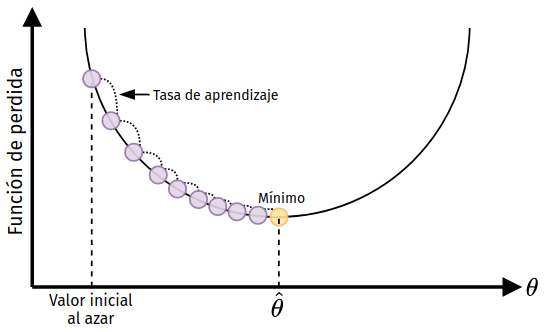
\includegraphics[width=0.58\textwidth]{023.png}
		\caption{Representación gráfica del descenso de gradiente.}
		\label{fig:gd}
	\end{center}
\end{figure}

Como vemos en la Fig~\ref{fig:lr}.Es importante ajustar apropiadamente el valor de la tasa de aprendizaje \textit{(learning rate)}. Si es demasiado pequeña, entonces el algoritmo tomará muchas iteraciones (pasos) para encontrar el mínimo. Por otro lado, si es muy alta, es posible que supere el mínimo y termine más lejos que cuando comenzó.

\begin{figure}[H]
	\begin{center}				
		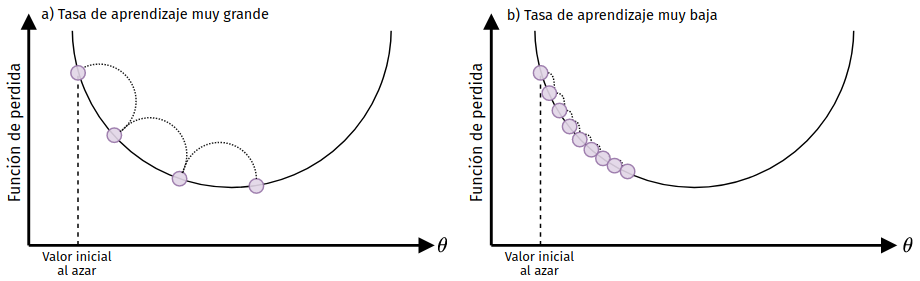
\includegraphics[width=1\textwidth]{tesis_37.png}
		\caption{Ajuste de la tasa de aprendizaje.}
		\label{fig:lr}
	\end{center}
\end{figure}

Por tanto para actualizar la matriz de pesos y de sesgo serán utilizadas las siguientes ecuaciones.

\begin{equation}
	W' = W - \alpha \frac{\partial J}{\partial W}
\end{equation}

\begin{equation}
	b' = b - \alpha \frac{\partial J}{\partial b}
\end{equation}

El $\alpha$ representa la tasa de aprendizaje o  \textit{learning rate}.

\subsection{Backpropagation}

Ya sabemos cómo fluyen las activaciones en la dirección hacia adelante. Tomamos las \textit{features} de entrada, las transformamos linealmente, aplicamos la activación sigmoidea en el valor resultante y finalmente tenemos nuestra activación que luego usamos para hacer una predicción \citep{sgd}.

Lo que veremos en esta sección es el flujo de gradientes a lo largo de la línea roja en la figura \ref{fig:back} mediante un proceso conocido como retropropagación o \textit{backpropagation}, que es esencialmente la regla de la cadena de cálculo aplicada a los gráficos computacionales.

\begin{figure}[H]
	\begin{center}				
		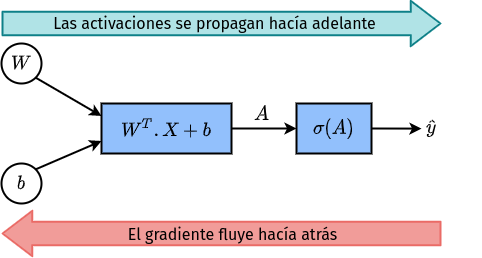
\includegraphics[width=0.65\textwidth]{024.png}
		\caption{Flujo de cálculo de las variables.}
		\label{fig:back}
	\end{center}
\end{figure}

Digamos que queríamos encontrar la derivada parcial de la variable $y$ con respecto a $x$ de la figura \ref{fig:func}. No podemos descubrirlo directamente porque hay otras 3 variables involucradas en el gráfico computacional. Entonces, hacemos este proceso iterativamente yendo hacia atrás en el gráfico de cálculo.

Primero descubrimos la derivada parcial de la salida $y$ con respecto a la variable $C$. Luego usamos la regla de la cadena de cálculo y determinamos la derivada parcial con respecto a la variable $B$ y así sucesivamente hasta que obtengamos la derivada parcial que estamos buscando.

\begin{figure}[H]
	\begin{center}				
		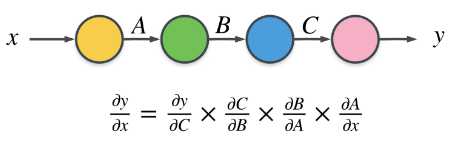
\includegraphics[width=0.8\textwidth]{025.png}
		\caption{Representación de grafo simple.}
		\label{fig:func}
	\end{center}
\end{figure}

Utilizando la función pérdida definida en la ecuación \ref{funcperdida} y reescribiéndola en su forma vectorial.

\begin{equation}
	J(\Theta)=\frac{1}{2} \|\hat{Y}-Y\|^2
\end{equation}

La derivada parcial de la función de pérdida con respecto a la activación de nuestro modelo es:

\begin{equation}
	\frac{\partial J}{\partial \hat{Y}}
	=\frac{1}{2} \frac{\partial J}{\partial \hat{Y}} \|\hat{Y}-Y\|^2 = \frac{1}{2} 2 \hat{Y} - Y \frac{\partial}{\partial \hat{Y}} (\hat{Y}-Y) = (\hat{Y}-Y) \frac{\partial}{\partial \hat{Y}} \|\hat{Y}-Y\| = (\hat{Y} - Y)
	\label{dj/dy}
\end{equation}

Avancemos un paso hacia atrás y calculemos nuestra próxima derivada parcial. Esto nos llevará un paso más cerca de los gradientes reales que queremos calcular.

Este es el punto donde aplicamos la regla de la cadena que mencionamos antes. Entonces, para calcular la derivada parcial de la función de pérdida con respecto a la salida transformada lineal, es decir, la salida de nuestro modelo antes de aplicar la activación sigmoidea:

\begin{equation}
	\frac{\partial J}{\partial D} = \frac{\partial J}{\partial \hat{Y}} \frac{\partial \hat{Y}}{\partial A}
	\label{dJdD}
\end{equation}

La primera parte de esta ecuación es el valor que habíamos calculado en la ecuación \ref{dj/dy}. Lo esencial para calcular aquí es la derivada parcial de la predicción de nuestro modelo con respecto a la salida transformada linealmente.

Veamos la ecuación para la predicción de nuestro modelo, la función de activación sigmoidea.

\begin{equation}
	\hat{Y} = sig(A) = \frac{1}{1+e^{-A}}
\end{equation}

Derivada de la salida final de nuestro modelo, \textit{i.e.} significa la derivada parcial de la función sigmoidea con respecto a su entrada.

\begin{equation}
	\frac{\partial}{\partial A} sig(A) = \frac{\partial}{\partial A} \frac{1}{1+e^{-A}} = \frac{\partial}{\partial A} (1+e^{-A})^{-1}
\end{equation}

\begin{equation}
	-1  (1+e^{-A})^{-2} \frac{\partial}{\partial A} (1+e^{-A}) = -1  (1+e^{-A})^{-2} (-e^{-A}) = \frac{e^{-A}}{(1+e^{-A})^2}
\end{equation}

Continuando, podemos simplificar aún más esta ecuación.

\begin{equation}
	\sigma(A) = \frac{1}{1+e^{-A}}
\end{equation}

\begin{equation}
	e^{-A} = \frac{1}{\sigma(A)} - 1 = \frac{1-\sigma(A)}{\sigma(A)}
\end{equation}

Substituyendo este valor en la ecuación \ref{dJdD} obtenemos:

\begin{equation}
	\frac{\partial J}{\partial A} = \frac{\partial J}{\partial \hat{Y}} \frac{e^{-A}}{(1+e^{-A})^2}
\end{equation}

\begin{equation}
	\frac{\partial J}{\partial A} = \frac{\partial J} {\partial \hat{Y} } \frac{1-\sigma(A)}{\sigma(A)} \sigma(A) \sigma(A)
\end{equation}

\begin{equation}
	\frac{\partial J}{\partial A} = \frac{\partial J} {\partial \hat{Y}} \sigma(A) (1-\sigma(A))
\end{equation}

Necesitamos la derivada parcial de la función de pérdida correspondiente a cada uno de los pesos. Pero como estamos recurriendo a la vectorización, podemos encontrarlo todo de una vez. Es por eso que hemos estado usando la notación mayúscula $W$ en vez de $w_1, w_2, \ldots, w_n$.

\begin{equation}
	\frac{\partial J}{\partial W} = \frac{\partial J}{\partial A} \frac{\partial A}{\partial W}
	\label{dJ/dW}
\end{equation}

\begin{equation}
	\frac{\partial J}{\partial b} = \frac{\partial J}{\partial A} \frac{\partial A}{\partial b}
	\label{dJ/db}
\end{equation}

La derivación de los pesos queda partiendo de la ecuación \ref{dJ/dW}:

\begin{equation}
	\frac{\partial J}{\partial W} = \frac{\partial J}{\partial A} \frac{\partial}{\partial W}(W^T X + b) = \frac{\partial J}{\partial A} X
\end{equation}

Y de la ecuación \ref{dJ/db}:

\begin{equation}
	\frac{\partial J}{\partial b} = \frac{\partial J}{\partial A} \frac{\partial}{\partial b}((W^T X + b) = \frac{\partial J}{\partial A} 1 = \frac{\partial J}{\partial A}
\end{equation}

Se demostró desde un punto de vista matemático el concepto de \textit{backpropagation} como se realiza la actualización de los pesos y sesgos utilizando el descenso por gradiente.

\clearpage

\subsection{Descenso de gradiente estocástico (SGD)}
El descenso de gradiente puede ser excepcionalmente lento en datasets muy grandes ya que en cada iteración se requiere calcular una predicción por cada punto en nuestro \textit{dataset} de entrenamiento, antes que actualicemos nuestra matriz de pesos.

En cambio lo que se utiliza es una variante de éste, el descenso de gradiente estocástico o \textit{Stochastic Gradient Descent (SGD)}.
El SGD es una simple modificación del algoritmo de descenso de gradiente estándar que computa el gradiente y actualiza la matriz de pesos $W$ en pequeños lotes o \textit{batches} de datos de entrenamiento, en vez del \textit{dataset} entero. Mientras esta modificación nos lleva a actualizaciones más "ruidosas", también nos permite tomar más pasos a lo largo del gradiente, llevando en ultima instancia a una convergencia más rápida y sin afectar negativamente a la pérdida y precisión del modelo.

En lugar de calcular nuestro gradiente en todo el conjunto de datos, en su lugar muestreamos nuestros datos, produciendo un lote. Evaluamos el gradiente en el lote y actualizamos nuestra matriz de peso $W$. Desde una perspectiva de implementación, también tratamos de aleatorizar nuestras muestras de entrenamiento antes de aplicar SGD ya que el algoritmo es sensible a los lotes.

En una implementación "purista" de SGD, el tamaño de su mini lote sería 1, lo que implica que muestrearíamos aleatoriamente un punto de datos del conjunto de entrenamiento, calcularíamos el gradiente
y actualizamos nuestros parámetros.

Sin embargo, a menudo utilizamos mini lotes que son mayores a 1. Los tamaños de lote típicos incluyen 32, 64, 128 y 256.

A continuación enumeramos las justificaciones a esta decisión.

\begin{enumerate}[noitemsep, topsep=2pt]
	\item Ayudan a reducir la variación en la actualización de parámetros, lo que conduce a una convergencia más estable. 
	\item Las potencias de dos a menudo son deseables para los tamaños de lote, ya que permiten que las bibliotecas de optimización de álgebra lineal interna sean más eficientes.
\end{enumerate}

En general, el tamaño del mini lote no es un hiperparámetro por el que debería preocuparse demasiado. Si está usando una GPU para entrenar su red neuronal, usted determina cuántos ejemplos de entrenamiento encajarán en su GPU y luego usa la potencia más cercana de dos, ya que el tamaño del lote se ajustará en la GPU. 

Para el entrenamiento de CPU, normalmente utiliza uno de los tamaños de lote enumerados anteriormente para asegurarse de cosechar los beneficios de las bibliotecas de optimización de álgebra lineal.

\subsection{Sobreajuste y bajo-ajuste}
El sobreajuste o \textit{overfitting} y la falta de ajuste o \textit{underfitting} \cite{quora} es muy importante para saber si el modelo predictivo está generalizando bien los datos o no. Un buen modelo debe poder generalizar bien los datos.

\begin{figure}[H]
	\begin{center}
		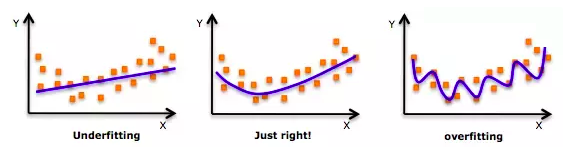
\includegraphics[width=1\textwidth]{026.png}
		\caption{Distintas representaciones del ajuste en un mismo modelo.}
		\label{fig:fitting}
	\end{center}
\end{figure}

En la figura \ref{fig:fitting} (derecha) el modelo está sobreajustado, \textit{i.e.} cuando funciona bien en el ejemplo de entrenamiento pero no funciona bien en datos no vistos. A menudo es el resultado de un modelo excesivamente complejo y ocurre porque el modelo está memorizando la relación entre el ejemplo de entrada (a menudo llamado $X$) y la variable objetivo (a menudo llamada $y$) o, por lo tanto, no puede generalizar bien los datos. El modelo de sobreajuste predice el objetivo en el conjunto de datos de entrenamiento con mucha precisión.

En cambio en la figura \ref{fig:fitting} (izquierda) se dice que el modelo predictivo tiene bajo-ajuste, si funciona mal en los datos de entrenamiento. Esto sucede porque el modelo no puede capturar la relación entre el ejemplo de entrada y la variable objetivo. Podría deberse a que el modelo es demasiado simple, es decir, las características de entrada no son lo suficientemente expresivas como para describir bien la variable objetivo. El modelo con bajo-ajuste no predice los objetivos en los conjuntos de datos de entrenamiento con mucha precisión.

Un buen modelo debe ser como el de la figura \ref{fig:fitting} (medio) que posee una buena precisión en su conjunto de datos de entrenamiento pero a su vez también tiene una buena \textit{performance} con datos que no haya visto.

\clearpage

\subsection{Regularización}
Para disminuir los efectos del sobreajuste se utiliza la \textbf{regularización} que después de la tasa de aprendizaje, es el parámetro más importante de su modelo que puede ajustar.

Existen varios tipos de técnicas de regularización, como la regularización L1, la regularización L2 (comúnmente llamada “pérdida de peso”) y Elastic Net, que se utilizan al actualizar la función de pérdida en sí, agregando un parámetro adicional para restringir la capacidad de el modelo.

La regularización nos ayuda a controlar la capacidad de nuestro modelo, asegurando que nuestros modelos sean mejores para hacer clasificaciones (correctas) en los puntos de datos en los que no fueron entrenados, lo que llamamos la capacidad de generalizar. Si no aplicamos la regularización, nuestros clasificadores pueden volverse demasiado complejos y ajustarse fácilmente a nuestros datos de entrenamiento, en cuyo caso perdemos la capacidad de generalizar a nuestros datos de prueba.

\subsection{Los cuatro ingredientes de una red neuronal}
Hay cuatro ingredientes principales \citep{rosebrock2017deep} que necesita para armar su propia red neuronal y algoritmo de aprendizaje profundo: un conjunto de datos, un modelo/arquitectura, una función de pérdida y una optimización.
\subsubsection{Conjunto de datos}
También llamado \textit{dataset}, es el primer ingrediente en el entrenamiento de una red neuronal: los datos en sí mismos junto con el problema que estamos tratando de resolver definen nuestros objetivos finales.

La combinación de su conjunto de datos y el problema que está tratando de resolver influye en su elección en la función de pérdida, la arquitectura de red y el método de optimización utilizado para entrenar el modelo. Por lo general, tenemos pocas opciones en nuestro conjunto de datos (a menos que esté trabajando en un proyecto de pasatiempo): se nos da un conjunto de datos con cierta expectativa sobre cuáles deberían ser los resultados de nuestro proyecto. Depende de nosotros entrenar un modelo de aprendizaje automático en el conjunto de datos para que funcione bien en la tarea dada.

\subsubsection{Función de pérdida}
Dado nuestro conjunto de datos y el objetivo, necesitamos definir una función de pérdida que se alinee con el problema que estamos tratando de resolver.

\subsubsection{Modelo/Arquitectura}
La arquitectura de su red puede considerarse la primera "elección" real que tiene que hacer como ingrediente. Es probable que su conjunto de datos sea elegido para usted (o al menos ha decidido que desea trabajar con un conjunto de datos determinado). Y si está realizando una clasificación, probablemente utilizará la entropía cruzada como su función de pérdida.
Sin embargo, su arquitectura de red puede variar dramáticamente, especialmente cuando con qué método de optimización elige entrenar su red.

\subsubsection{Método de optimización}
El ingrediente final es definir un método de optimización. El SGD se usa con bastante frecuencia.
SGD sigue siendo el caballo de batalla del aprendizaje profundo: la mayoría de las redes neuronales se entrenan a través de SGD, aunque existen otros métodos de optimización como Adam.
Luego debe establecer una tasa de aprendizaje adecuada, la fuerza de regularización y el número total de épocas para las que se debe entrenar la red.

\clearpage

\section{Redes neuronales convolucionales}
Las redes neuronales convolucionales \citep{rosebrock2017deep} (\textit{CNNs} en Inglés) son principalmente útiles si en la entrada los datos presentados son imágenes, permite el desarrollo de modelos supervisados y no supervisados.

Podemos definir una \textit{CNN} como una red neuronal que cambia una capa totalmente conectada (\textit{fully-connected}) por una convolucional para al menos una de las capas de la red.

Cada capa en una \textit{CNN} aplica un conjunto de filtros, usualmente cientos o miles de ellos y combinan los resultados, alimentando la entrada de la siguiente capa de la red. Durante el entrenamiento, una \textit{CNN} automáticamente aprende los valores para esos filtros.

En el contexto de la clasificación de imágenes, una \textit{CNN} puede aprender a:
\begin{itemize}[noitemsep, topsep=2pt]
	\item Detectar bordes a partir de datos de píxeles sin procesar en la primera capa.
	\item Usar esos bordes para detectar formas (\textit{i.e. blobs}) en la segunda capa.
	\item Usar esas formas para detectar características de alto nivel tales como estructuras faciales, partes de un auto, etc. en las capas de más alto nivel.
\end{itemize}

La última capa en una \textit{CNN} usa esas características de alto nivel para realizar predicciones considerando los contenidos de una imagen.

Las \textit{CNNs} nos dan dos beneficios claves con respecto al reconocimiento de imágenes:
\begin{itemize}[noitemsep, topsep=2pt]
	\item \textbf{invariancia local}: nos permite clasificar una imagen que contiene un objeto particular sin importar donde aparece éste en la imagen.
	\item \textbf{composicionalidad}: cada filtro compone un parche local de características de nivel inferior en una representación de nivel superior, similar a cómo podemos componer un conjunto de funciones matemáticas que se basan en la salida de funciones anteriores. Esta composición permite que nuestra red aprenda características más ricas de forma más profunda.
	      	      	      
\end{itemize}

Las convoluciones bi-dimensionales (2D) son usadas para tratar las imágenes, mientras que las convoluciones unidimensionales (1D) nos permiten analizar entradas secuenciales, obteniendo la información con dependencias temporales. Entonces al combinar estas dos técnicas, se puede apreciar cómo evolucionan en el tiempo las imágenes capturadas y así hacer predicciones a futuro.

\subsection{Convolución 1D}
Si $f$ y $g$ son funciones discretas \citep{keller}, entonces $f * g$ es la convolución de $f$ y $g$ y está definida como:

$$(f*g)(x)=\sum_{u=-\infty}^{\infty} f(u)g(x-u)$$

Intuitivamente, la convolución de dos funciones representa la cantidad de superposición entre estas. La función $g$ es la entrada y $f$ el \textit{kernel} o núcleo de la convolución.

Sin embargo en los algoritmos de \textit{machine learning} lo que manejamos usualmente son vectores o arreglos de tal forma que nos resultará más provechoso analizar la convolución entre ellos.

Si la función $f$ varía sobre un conjunto finito de valores $a = a_1, a_2, \dots, a_n$ entonces puede ser representado como el vector 
$\begin{bmatrix} a_1 & a_2 & \cdots & a_n \end{bmatrix}$.

Si las funciones $f$ y $g$ son representadas como vectores $a = \begin{bmatrix} a_1 & a_2 & \cdots & a_m \end{bmatrix}$ y $b = \begin{bmatrix} b_1 & b_2 & \cdots & b_n \end{bmatrix}$, entonces $f*g$ es un vector $c = \begin{bmatrix} c_1 & c_2 & \cdots & c_{m+n-1} \end{bmatrix}$ definido de la siguiente forma:

$$ c = \sum_{u} a_u b_{x-u+1}$$

donde $u$ abarca todos los subíndices legales para $a_u$ y $b_{x-u+1}$, específicamente $u=max(1, x-n+1)\dots min(x,m).$

Lo que puede parecer complicado en la teoría no lo es en la práctica, observemos la Fig.~\ref{fig:conv1dk1} \citep{Cogneethi2019Aug}. El vector \textit{input} también se denomina vector de características y el vector \textit{output} mapa de características.

Lo que sucede es que si el \textit{kernel} tiene un único valor sólo es necesario multiplicarlo por cada valor del vector \textit{input} y guardarlo en el índice correspondiente del vector \textit{output}.

\begin{figure}[H]
	\begin{center}				
		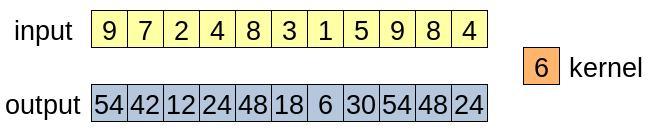
\includegraphics[width=0.65\textwidth]{tesis_24.png}
		\caption{Vectores de convolución unidimensional con kernel simple.}
		\label{fig:conv1dk1}
	\end{center}
\end{figure}

En cambio si tenemos un \textit{kernel} de dimensiones $2 \times 1$ como la Fig.\ref{fig:conv1dk2} para obtener el valor de salida $i$ debemos usar los valores de entrada $i$ y su vecino $i+1$.

Para obtener el primer valor del vector de salida se realizó la operación \texttt{o[0] = i[0]k[0] + i[1]k[1] = 69}. De esta forma iteramos a lo largo de todo el vector de entrada hasta obtener todos los valores de salida. Podemos notar que el tamaño del vector de salida es menor ahora, a medida que aumentamos el tamaño del kernel disminuye el del vector de salida.

\begin{figure}[H]
	\begin{center}				
		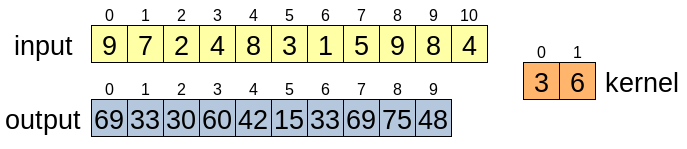
\includegraphics[width=0.7\textwidth]{tesis_25.png}
		\caption{Vectores de convolución unidimensional con kernel doble.}
		\label{fig:conv1dk2}
	\end{center}
\end{figure}

Con objeto de dejar totalmente en claro el algoritmo observemos la Fig.~\ref{fig:conv1dk3}. Para obtener el valor del índice 4 del vector de salida operamos \texttt{o[4] = i[4]k[0]+i[5]k[1]+i[6]k[2] = 23}.

\begin{figure}[H]
	\begin{center}				
		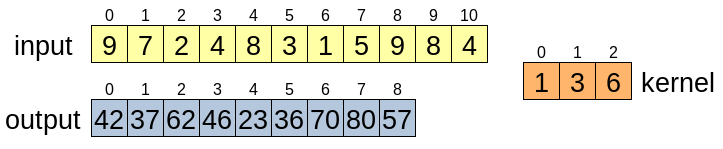
\includegraphics[width=0.75\textwidth]{tesis_26.png}
		\caption{Vectores de convolución unidimensional con kernel triple.}
		\label{fig:conv1dk3}
	\end{center}
\end{figure}

\subsection{Convolución 2D}

A su vez podemos extender esto a convoluciones para funciones de dos variables.

Si $f$ y $g$ son funciones discretas de dos variables, entonces $f*g$ es la convolución de $f$ y $g$ y se define:

$$
(f*g)(x,y) = \sum_{u=-\infty}^{+\infty} \sum_{v=-\infty}^{+\infty} f(u,v)g(x-u,y-v)
$$

Podemos considerar funciones de dos variables como matrices con $A_{xy} = f(x,y)$ y obtener una definición matricial de la convolución.

Si las funciones $f$ y $g$ son representadas como las matrices $A$ y $B$ con dimensiones de $n \times m$ y $k \times i$ respectivamente, entonces $f*g$ es una matriz $C$ de dimensiones $(n+k-1) \times (m+i-1)$ definida:

$$
c_{xy} = \sum_{u} \sum_{v} a_{uv} b_{x-u+1,y-v+1}
$$

donde $u$ y $v$ abarcan todos los subíndices posibles para $a_{uv}$ y $b_{x-u+1,y-v+1}$.

Así como notamos que el algoritmo para la convolución 1D no era tan complejo como su definición formal, lo mismo sucede para la convolución 2D pero extrapolando el mecanismo a una dimensión más.

En la Fig.~\ref{fig:conv2d} \citep{andrianaivo2019architecture} analizamos el procedimiento. Se debe centrar el kernel $K$ sobre el primer valor a calcular, para luego realizar las respectivas multiplicaciones y luego guardarlas en la matriz de salida $O$, de esta manera iremos iterando de izquierda a derecha y de arriba hacia abajo toda la matriz $I$.

\begin{figure}[H]
	\begin{center}				
		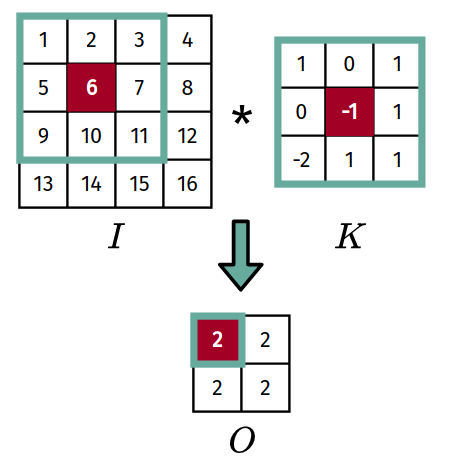
\includegraphics[width=0.5\textwidth]{convolution2d.png}
		\caption{Vectores de convolución bidimensional con kernel $3 \times 3$.}
		\label{fig:conv2d}
	\end{center}
\end{figure}

Consideremos la Fig.~\ref{fig:conv2dimg} \citep{Saha2020Oct}, tenemos una imagen RGB que ha sido separada por sus tres canales de color: rojo, verde y azul. Hay varios espacios de color en los que existen las imágenes: escala de grises, RGB, HSV, CMYK, etc.

\begin{figure}[H]
	\begin{center}				
		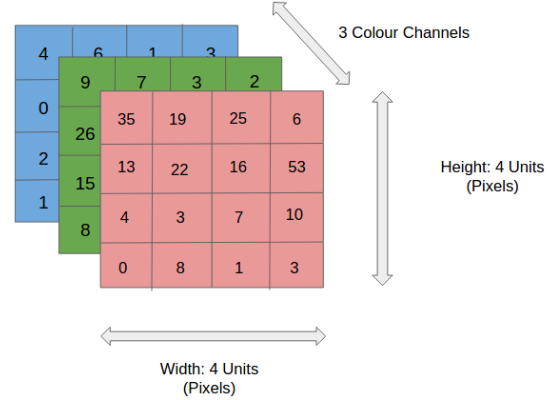
\includegraphics[width=0.45\textwidth]{imgrgb.png}
		\caption{Imagen RGB $4 \times 4 \times 3$.}
		\label{fig:conv2dimg}
	\end{center}
\end{figure}

Si consideramos la totalidad de la imagen como un prisma donde la profundidad corresponde a cada canal de color, podemos ver en la figura~\ref{fig:kernelmove} el movimiento que realiza el kernel (con forma de cubo) a través del volumen del prisma.

\begin{figure}[H]
	\begin{center}				
		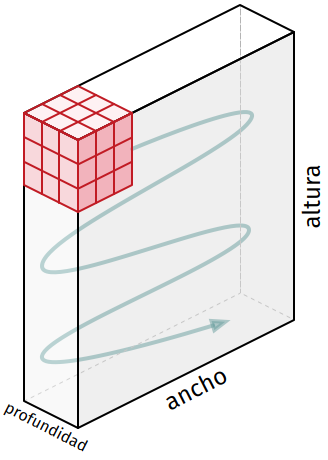
\includegraphics[width=0.25\textwidth]{kernelmove.png}
		\caption{Movimiento del \textit{kernel}.}
		\label{fig:kernelmove}
	\end{center}
\end{figure}

\subsubsection{\textit{Padding}}

Un problema a abordar al aplicar la convolución es que tendemos a perder píxeles en el perímetro de nuestra imagen (o vector). Dado que normalmente usamos núcleos pequeños, para cualquier convolución dada, es posible que solo perdamos unos pocos píxeles, pero esto puede sumarse a medida que aplicamos muchas capas convolucionales sucesivas. 

\clearpage
Una solución sencilla a este problema es agregar píxeles adicionales de relleno (\textit{padding}) alrededor del límite de nuestra imagen de entrada, aumentando así el tamaño efectivo de la imagen. Normalmente, establecemos los valores de los píxeles adicionales en cero. \citep{padding}

En la figura~\ref{fig:padding}, rellenamos una entrada de $3 \times 3$, aumentando su tamaño a $5 \times 5$. La salida correspondiente aumenta entonces a una matriz de $4 \times 4$.

\begin{figure}[H]
	\begin{center}				
		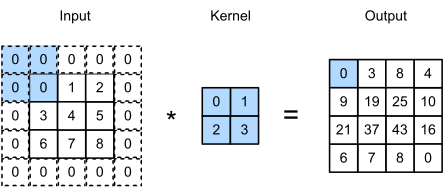
\includegraphics[width=0.50\textwidth]{conv-pad.png}
		\caption{Relleno o \textit{padding}.}
		\label{fig:padding}
	\end{center}
\end{figure}

\subsubsection{\textit{Stride}}

Al realizar la convolución, comenzamos con la ventana en la esquina superior izquierda del tensor de entrada y luego la deslizamos sobre todas las ubicaciones, tanto hacia abajo como hacia la derecha. Usualmente deslizamos un elemento a la vez. Sin embargo, a veces, ya sea por eficiencia computacional o porque deseamos reducir la resolución, movemos nuestra ventana más de un elemento a la vez, omitiendo las ubicaciones intermedias.

Nos referimos al número de filas y columnas atravesadas por diapositiva como la zancada o \textit{stride}. Hasta ahora, hemos utilizado \textit{stride} de 1, tanto para altura como para ancho. A veces, es posible que deseemos usar un paso más grande, como en la figura~\ref{fig:stride} \citep{Saha2020Oct}.

\begin{figure}[H]
	\begin{center}				
		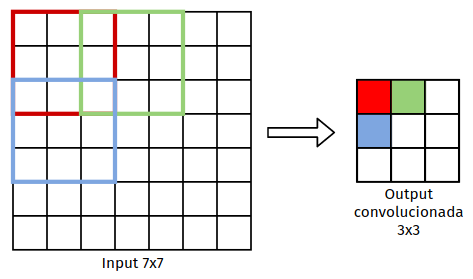
\includegraphics[width=0.6\textwidth]{tesis_44.png}
		\caption{Convolución con \textit{stride} de 2.}
		\label{fig:stride}
	\end{center}
\end{figure}

\subsubsection{Tamaño del vector de salida de una convolución}

Está determinado por la siguiente formula \citep{SOOutputConv}:

$$ output_{size} = \frac{W-F+2P}{S+1}$$

donde $W = input_{size}$, $F=kernel_{size}$, $P$=\textit{padding} y $S$=\textit{stride}.

\subsection{Tipos de capas}
Existen varias tipos de capas usadas \citep{rosebrock2017deep} para construir \textit{CNNs} pero las más comunes incluyen:

\begin{itemize}[noitemsep, topsep=2pt]
	\item Convolucional (\texttt{CONV})
	\item Activación (\texttt{ACT})
	\item \textit{Pooling} (\texttt{POOL})
	\item \textit{Fully-connected} (\texttt{FC})
	\item \texttt{\textit{Dropout}} (\texttt{DO})
\end{itemize}

Apilando estas capas de una manera específica producimos una \textit{CNN}. De estos tipos de capas, \texttt{CONV} y \texttt{FC} (y en menor medida, \texttt{BN}) son las únicas capas que contienen parámetros que se aprenden durante el proceso de entrenamiento.

Las capas \texttt{ACT} y \texttt{DO} no se consideran verdaderas capas en sí mismas, pero a menudo se incluyen en los diagramas de red para que la arquitectura sea explícitamente clara.

Las capas (\texttt{POOL}), de igual importancia que \texttt{CONV} y \texttt{FC}, también se incluyen en los diagramas de red, ya que tienen un impacto sustancial en las dimensiones espaciales de un
imagen mientras se mueve a través de una \textit{CNN}.

\subsubsection{Convolución}

La capa convolucional (\texttt{CONV}) es el componente básico de una red neuronal convolucional. Los parámetros de la capa \texttt{CONV} consisten en un conjunto de $K$ \textit{kernels} entrenables, donde cada uno tiene un ancho y un alto, y casi siempre son cuadrados. 

Una capa o filtro puede tener varios \textit{kernels} que al convolucionar con el vector de entrada (que podría ser una imagen) producen mapas de características (\textit{features map}).

\begin{figure}[H]
	\begin{center}				
		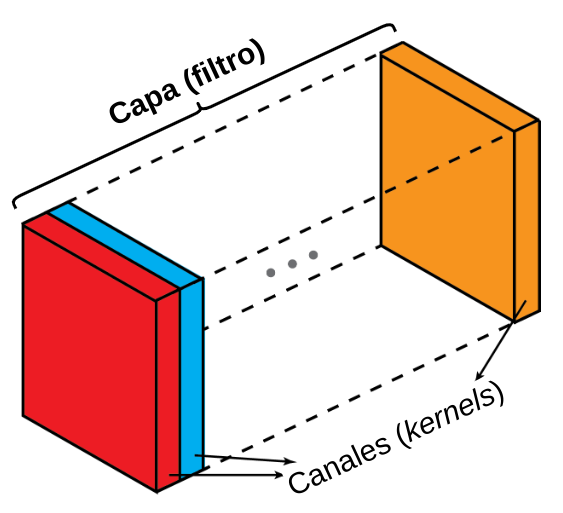
\includegraphics[width=0.45\textwidth]{layer-kernels.png}
		\caption{Una capa está compuesta de una colección de \textit{kernels}.}
		\label{fig:layer-kernel}
	\end{center}
\end{figure}

La línea que divide los conceptos de filtro y \textit{kernel} es un poco difusa. A veces, se usan indistintamente, lo que podría crear confusiones. Esencialmente, estos dos términos tienen una sutil diferencia. Un "\textit{kernel}" se refiere a una matriz 2D de pesos. El término "filtro" se refiere a estructuras 3D de varios \textit{kernels} apilados juntos. Para un filtro 2D, el filtro es igual que el kernel. Pero para un filtro 3D y la mayoría de las convoluciones en el aprendizaje profundo, un filtro es una colección de \textit{kernels} (fig.~\ref{fig:layer-kernel}). Cada \textit{kernel} es único, enfatizando diferentes aspectos del canal de entrada.

El funcionamiento de la capa convolucional se resume en pensar en cada uno de los $K$ \textit{kernels} deslizándose a través del vector de entrada, computando un producto de Hadamard, sumando cada uno de sus valores y luego almacenando el valor generado en un mapa 2D de activación. En la figura~\ref{fig:conv-mechanism} se puede observar una visualización de la secuencia.

\begin{figure}[H]
	\begin{center}				
		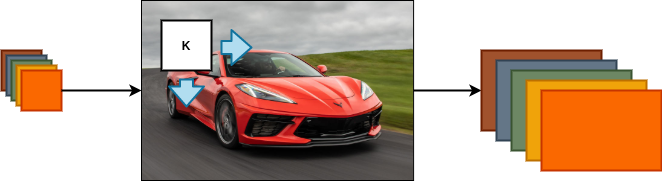
\includegraphics[width=1\textwidth]{feature-map-clean.png}
		\caption{\textbf{Izquierda:} en cada capa convolucional de una \textit{CNN}, hay $K$ \textit{kernels} distintos. \textbf{Medio:} Cada uno de los \textit{kernels} es convolucionado con el vector de entrada. \textbf{Derecha:} Cada \textit{kernel} produce una salida 2D, llamada mapa de activación o \textit{features}.}
		\label{fig:conv-mechanism}
	\end{center}
\end{figure}

Luego de aplicar los $K$ filtros al vector de entrada, ahora tenemos $K \times 2D$ mapas de activación. Luego apilamos nuestro $K$ mapas de activación a través de la dimensión de profundidad de nuestra matriz para formar el volumen final de salida (figura~\ref{fig:k-maps}).

\begin{figure}[H]
	\begin{center}				
		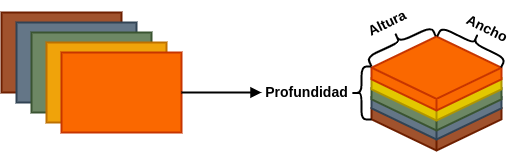
\includegraphics[width=0.8\textwidth]{k-activation-map.png}
		\caption{Luego de obtener los $K$ mapas de activación, son apilados juntos para formar el volumen de entrada a la siguiente capa en la red.}
		\label{fig:k-maps}
	\end{center}
\end{figure}

Cada entrada en el volumen de salida es, por tanto, una salida de una neurona que "observa" sólo una pequeña región de la entrada. De esta manera, la red "aprende" los filtros que se activan cuando ven un tipo específico de característica en una ubicación espacial determinada en el volumen de entrada.

En las capas inferiores de la red, los filtros pueden activarse cuando ven regiones con forma de borde o de esquina. Luego, en las capas más profundas de la red, los filtros pueden activarse en presencia de características de alto nivel, como partes de la cara, la pata de un perro, el capó de un automóvil, etc.

\subsubsection{Activación}

Luego de cada capa \texttt{CONV} en una \textit{CNN}, normalmente aplicamos una función no lineal, como ReLU, ELU, etc (se ejemplifica en la figura~\ref{fig:relu-act}). Las capas \texttt{ACT} no son técnicamente "capas" (debido al hecho de que no se aprenden parámetros/pesos dentro de una capa de activación) y, a veces, se omiten en los diagramas de arquitectura de red, ya que se supone que una activación sigue inmediatamente a una convolución.

\begin{figure}[H]
	\begin{center}				
		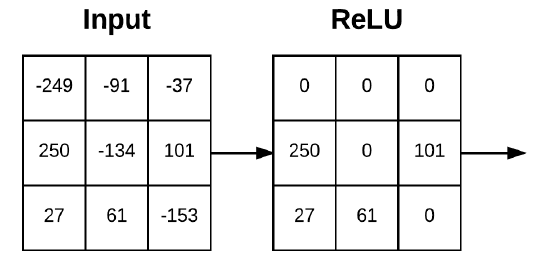
\includegraphics[width=0.65\textwidth]{tesis_47.png}
		\caption{Un ejemplo de un volumen de entrada desplazándose a través de una \texttt{ACT} ReLU.}
		\label{fig:relu-act}
	\end{center}
\end{figure}

\subsubsection{\textit{Fully-connected}}
Las neuronas en las capas \texttt{FC} están totalmente conectadas a todas las activaciones de la capa anterior, como en una red neuronal \textit{feed-forward}. Siempre se ubican al final de la red.

\subsubsection{\textit{Pooling}}

Similar a la capa convolucional, la capa de \texttt{POOL} es responsable de reducir el tamaño espacial de la entidad convolucionada. Esto es para disminuir la potencia computacional requerida para procesar los datos a través de la reducción de dimensionalidad. Además, es útil para extraer características dominantes que son invariantes rotacionales y posicionales, manteniendo así el proceso de entrenamiento efectivo del modelo.

Existen dos tipos:
\begin{itemize}[noitemsep, topsep=2pt]
	\item \textit{Max pooling} (\texttt{MPOOL}): devuelve el valor máximo de la parte de la imagen cubierta por el \textit{kernel} (figura \ref{fig:type-pooling} arriba).
	\item \textit{Average pooling} (\texttt{APOOL}): devuelve el promedio de todos los valores de la parte de la imagen cubierta por el \textit{kernel} (figura \ref{fig:type-pooling} abajo).
\end{itemize}

\begin{figure}[H]
	\begin{center}				
		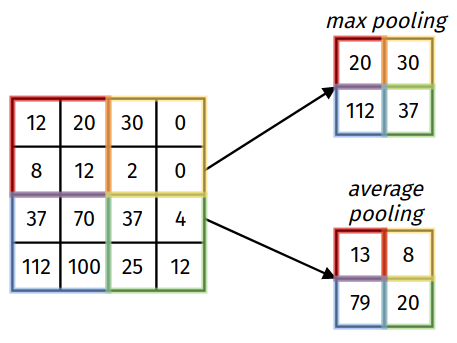
\includegraphics[width=0.5\textwidth]{tesis_45.png}
		\caption{Tipos de \textit{pooling}.}
		\label{fig:type-pooling}
	\end{center}
\end{figure}

Cabe destacar que \texttt{MAXPOOL} también actúa como supresor de ruido ya que descarta las activaciones ruidosas por completo además de la reducción de dimensionalidad. Por otro lado, el \texttt{AVGPOOL} simplemente realiza la reducción de dimensionalidad como un mecanismo de supresión de ruido. Por lo tanto, podemos decir que \texttt{MAXPOOL} funciona mucho mejor que \texttt{AVGPOOL}.

\subsubsection{\textit{Batch Normalization}}

Las capas de normalización por lotes o \textit{Batch Normalization} (\texttt{BN}), como su nombre indica, se utilizan para normalizar las activaciones de un volumen de entrada determinado antes de pasarlo a la siguiente capa de la red.

Por lo general, para entrenar una red neuronal, realizamos un preprocesamiento de los datos de entrada, por ejemplo, normalizar todos los datos para que se parezcan a una distribución normal (es decir, media cero y una varianza unitaria). Algunas razones para realizar esto puede ser prevenir la saturación temprana de funciones de activación no lineales como la función sigmoidea, asegurar que todos los datos de entrada estén en el mismo rango de valores, etc. \citep{bn}

Pero el problema aparece en las capas intermedias porque la distribución de las activaciones cambia constantemente durante el entrenamiento. Esto ralentiza el proceso de entrenamiento porque cada capa debe aprender a adaptarse a una nueva distribución en cada paso del entrenamiento. Este problema se conoce como \textbf{cambio de covariables interno}.

Podemos utilizar la normalización por lotes o \textit{Batch Normalization} (\texttt{BN}) como un método para normalizar las entradas de cada capa para así forzarlo a tener aproximadamente la misma distribución en cada paso de entrenamiento, con el fin de combatir el problema expresado anteriormente.

Durante el tiempo de entrenamiento, una capa de normalización por lotes se obtiene el promedio y la varianza del lote:

$$ \mu_{\beta} = \frac{1}{m} \sum_{i=1}^m x_i $$

$$ \sigma_{\beta}^2 = \frac{1}{m}  \sum_{i=1}^m (x_i - \mu_{\beta} ) ^2$$

Normalizamos las entradas de la capa usando las estadísticas del lote calculados previamente:

$$ \bar{x_i} = \frac{x_i - \mu_{\beta}}{\sqrt{\sigma_{\beta}^2+\epsilon}} $$

%Escalamos y \textit{shifteamos} en orden para obtener la salida de la capa:

%$$ y_i = \gamma \hat{x_i} + \beta $$

Establecemos $1e-7 \leq \epsilon \leq 0$ para evitar sacar la raíz cuadrada de cero. Aplicar esta ecuación implica que las activaciones que salen de una capa \texttt{BN} tendrán una media y una varianza unitaria aproximadamente cero (es decir, centrada en cero).
Reemplazamos el mini-lote $\mu_{\beta}$ y $\sigma_{\beta}$ con promedios de $\mu_{\beta}$ y $\sigma_{\beta}$ calculados durante el proceso de entrenamiento. Esto asegura que podemos pasar vectores a través de nuestra red y aún así obtener predicciones precisas sin ser sesgados por $\mu_{\beta}$ y $\sigma_{\beta}$ del mini-lote final pasado a través de la red en el momento del entrenamiento. 

La \texttt{BN} también tiene el beneficio adicional de ayudar a "estabilizar" el entrenamiento, lo que permite una mayor variedad de tasas de aprendizaje y fortalezas de regularización. Esto no alivia la necesidad de ajustar estos parámetros, por supuesto, pero le facilitará la vida al hacer que la tasa de aprendizaje y la regularización sean menos volátiles y más fáciles de ajustar. También tenderá a notar pérdidas finales más bajas y una curva de pérdida más estable en sus redes.

\subsubsection{\textit{Dropout}}
El \textit{dropout} (\texttt{DO}) es en realidad una forma de regularización que tiene como objetivo ayudar a prevenir el sobreajuste aumentando la precisión de las pruebas, quizás a expensas de la precisión del entrenamiento. \citep{rosebrock2017deep}

La razón está en reducir el sobreajuste alterando de forma explicita la arquitectura de la red en tiempo de entrenamiento. La desconexión aleatoria de las conexiones garantiza que ningún nodo de la red sea responsable de la activación cuando se le presenta un patrón determinado. El \texttt{DO} garantiza que haya múltiples nodos redundantes que se activarán cuando se les presenten entradas similares (lo que a su vez ayuda a que nuestro modelo a generalizar).

\begin{figure}[H]
	\begin{center}
		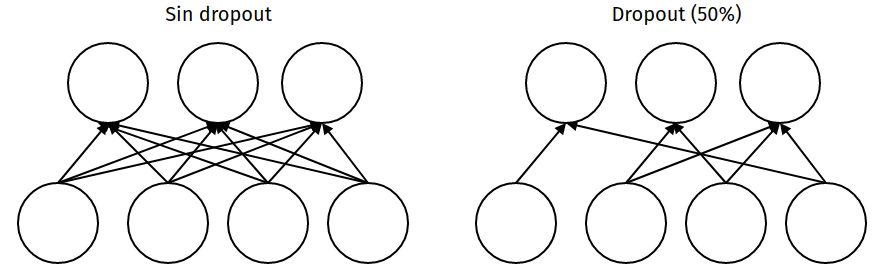
\includegraphics[width=0.9\textwidth]{tesis_46.png}
		\caption{\textbf{Izquierda:} Dos capas \texttt{FC} sin \texttt{DO}. \textbf{Derecha:} Las mismas dos capas luego de realizar \textit{dropout} sobre la mitad de las conexiones.}
		\label{fig:type-pooling}
	\end{center}
\end{figure}

\subsection{\textit{WaveNet} y capas convolucionales causales dilatadas}

\textit{WaveNet} es una red neuronal profunda para generar audio muestra a muestra. La arquitectura de este modelo permite aprovechar las eficiencias de las capas de convolución al mismo tiempo que alivia el desafío de aprender las dependencias a largo plazo en una gran cantidad de pasos de tiempo (más de 1000) \citep{wavenet2}.

Se optó por estudiar este modelo dado que funciona con series temporales y trata de anticipar patrones de comportamiento causados por patrones de comportamiento previos, lo que se puede correlacionar con la naturaleza de los datos a tratar.

En el núcleo de \textit{WaveNet} se encuentra la \textbf{capa de convolución causal dilatada} (figura~\ref{fig:causal-conv}), que le permite tratar adecuadamente el orden temporal y manejar las dependencias a largo plazo sin una explosión en la complejidad del modelo. \citep{wavenet}

\begin{figure}[H]
	\begin{center}				
		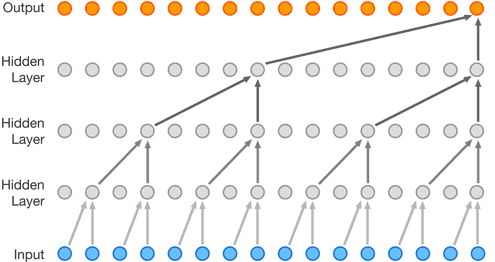
\includegraphics[width=0.8\textwidth]{causal-conv.png}
		\caption{Paso de la información a través de la capa de convolución causal dilatada. \citep{wavenet2}}
		\label{fig:causal-conv}
	\end{center}
\end{figure}

En una capa de convolución unidimensional tradicional, deslizamos un filtro de pesos a través de una serie de entrada, aplicándolo secuencialmente a las regiones (generalmente superpuestas) de la serie. Pero cuando utilizamos el historial de una serie temporal para predecir su futuro, debemos tener cuidado. A medida que formamos capas que eventualmente conectan los pasos de entrada a las salidas, debemos asegurarnos de que las entradas no influyan en los pasos de salida que los siguen a tiempo. De lo contrario, estaríamos usando el futuro para predecir el pasado, lo que sería hacer trampa.

Para asegurarnos de no hacer trampa de esta manera, ajustamos nuestro diseño de convolución para prohibir explícitamente que el futuro influya en el pasado. En otras palabras, solo permitimos que las entradas se conecten a salidas de pasos de tiempo futuros en una estructura \textbf{causal}, como se muestra a continuación en una visualización del documento WaveNet. En la práctica, esta estructura 1D causal es fácil de implementar desplazando las salidas convolucionales tradicionales en varios pasos de tiempo.

\begin{figure}[H]
	\begin{center}				
		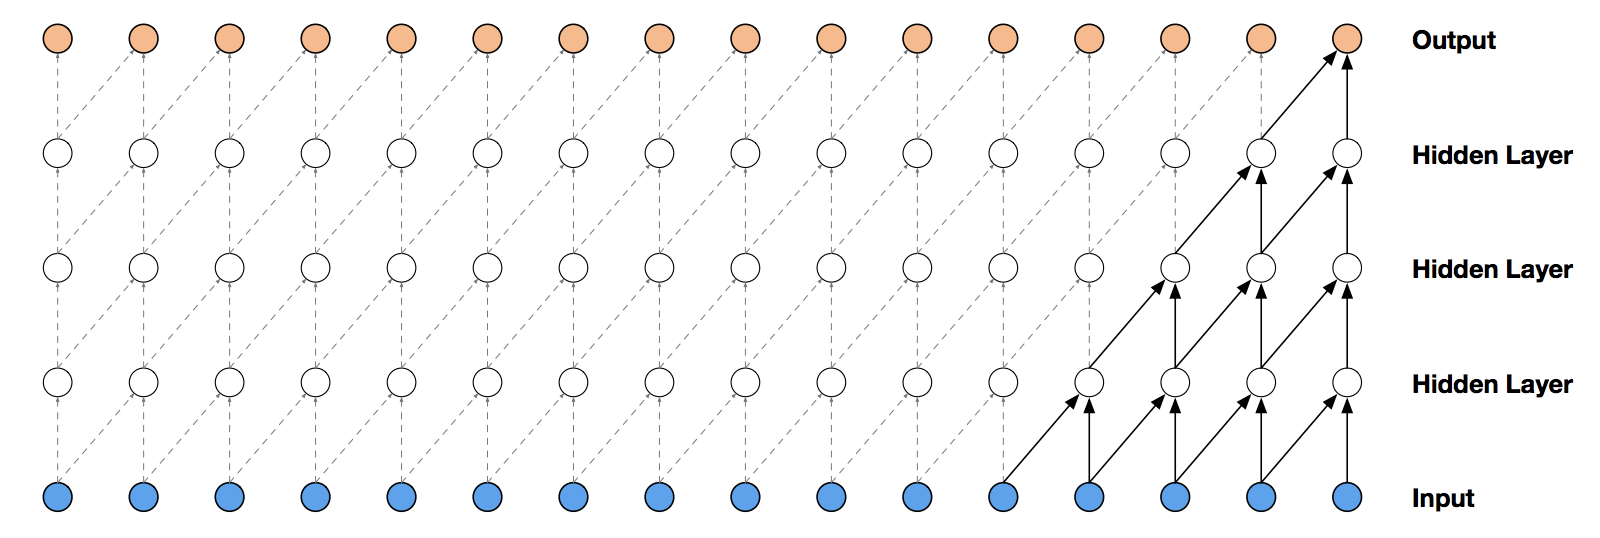
\includegraphics[width=1\textwidth]{stackcausal-conv.png}
		\caption{Visualización de una pila de capas causales convoluciones. \citep{wavenet2}}
		\label{fig:stackcausal-conv}
	\end{center}
\end{figure}

Las convoluciones causales proporcionan la herramienta adecuada para manejar el flujo temporal, pero necesitamos una modificación adicional para manipular adecuadamente las dependencias a largo plazo. En la figura \ref{fig:stackcausal-conv} de convolución causal simple, puede ver que solo los 5 pasos de tiempo más recientes pueden influir en la salida resaltada. De hecho, necesitaríamos una capa adicional por paso de tiempo para llegar más atrás en la serie (para usar la terminología adecuada, para aumentar el \textbf{campo receptivo de la salida}). Con una serie de tiempo que tiene una gran cantidad de pasos, el uso de convoluciones causales simples para aprender de toda la historia rápidamente haría un modelo demasiado complejo computacional y estadísticamente.

\begin{figure}[H]
	\begin{center}				
		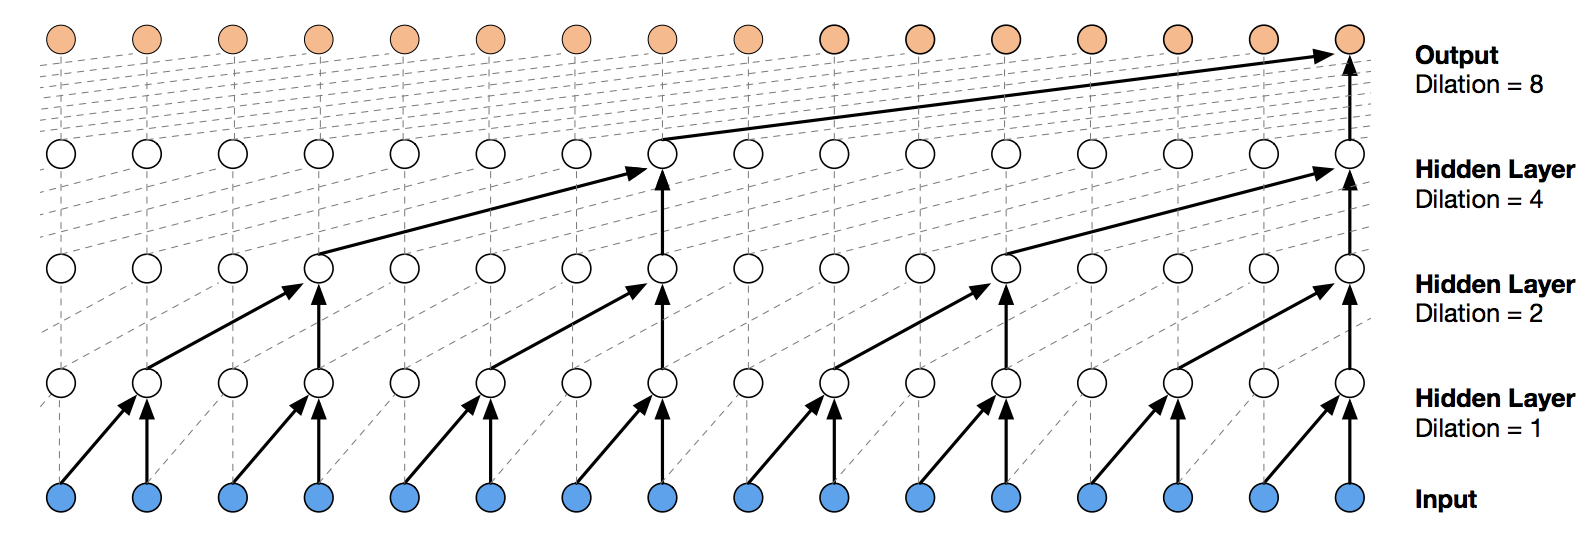
\includegraphics[width=1\textwidth]{dilated-conv.png}
		\caption{Visualización de una pila de capas causales convoluciones dilatadas. \citep{wavenet2}}
		\label{fig:dilated-conv}
	\end{center}
\end{figure}

En lugar de cometer ese error, \textit{WaveNet} utiliza \textbf{convoluciones dilatadas}, que permiten que el campo receptivo aumente exponencialmente en función de la profundidad de la capa de convolución. 

En una capa de convolución dilatada, los filtros no se aplican a las entradas de una manera secuencial simple, sino que omiten una entrada de tasa de dilatación constante entre cada una de las entradas que procesan, como en el diagrama \textit{WaveNet} a continuación. Al aumentar la tasa de dilatación multiplicativamente en cada capa (por ejemplo, 1, 2, 4, 8,…), podemos lograr la relación exponencial entre la profundidad de la capa y el tamaño del campo receptivo que deseamos. 

En la figura~\ref{fig:dilated-conv}, puede ver cómo ahora solo necesitamos 4 capas para conectar los 16 valores de la serie de entrada a la salida resaltada (digamos, el valor de paso de tiempo 17). Por extensión, cuando se trabaja con una serie de tiempo diaria, se puede capturar más de un año de historia con solo 9 capas de convolución dilatadas de esta forma.

\clearpage

\section{Redes neuronales recurrentes}
Anteriormente hemos visto cómo las redes neuronales ó convolucionales nos permiten clasificar un dato, por ejemplo una palabra, un sonido, o una imagen, pero tienen un inconveniente, y es que cuando tenemos una secuencia de datos (\textit{e.g.} una secuencia de palabras o una secuencia de imágenes) este tipo de arquitecturas no pueden procesar ese tipo de datos. 

Las Redes Neuronales Recurrentes \textit{(RNN)} \citep{karpathy:rnn} resuelven este inconveniente, porque son capaces de procesar diferentes tipos de secuencias, como textos, conversaciones, vídeos, música, y además de eso no sólo clasifican los datos como lo hacen las redes neuronales o convolucionales, sino que también poseen la capacidad de generar nuevas secuencias.

Si a una red neuronal o convolucional se le presenta una imagen o una palabra, con el entrenamiento adecuado estas arquitecturas lograrán clasificar un sinnúmero de datos, logrando a la vez una alta precisión. 

?`Pero qué sucede si en lugar de una única imagen o palabra se introduce a la red una secuencia de imágenes, es decir un vídeo, o una secuencia de palabras (una conversación)? En este caso en ninguna de estas redes será capaz de procesar los datos por dos motivos:
\begin{itemize}[noitemsep, topsep=2pt]
	\item Estas arquitecturas están diseñadas para que los datos de entrada y de salida siempre tengan el mismo tamaño; sin embargo, un vídeo o una conversación se caracterizan por ser un tipo de datos con un tamaño variable: una cantidad variable de "frames"
	      en el caso del vídeo o una cantidad variable de palabras en el caso de la conversación. 
	\item En un vídeo o en una conversación los datos están \textbf{correlacionados}, esto quiere decir que la siguiente palabra pronunciada o la siguiente imagen en la secuencia de vídeo dependerá de la palabra o imagen anterior. E incluso estas palabras e imágenes estarán relacionadas con aquellas que se presenten más adelante en la secuencia y una \textit{NN} ó \textit{CNN} no está en capacidad de analizar la relación entre varias palabras o imágenes de la secuencia.
\end{itemize}

Una secuencia es una serie de datos que siguen un orden específico y tienen únicamente significado cuando se analizan en conjunto y no de manera individual. Dichos datos, analizados de forma individual o en un orden diferente, carecen de significado. Es evidente que una secuencia no tiene un tamaño predefinido pues no podemos saber con antelación el número de datos. 

\clearpage

Las \textit{RNN} resuelven los inconvenientes expresados anteriormente, pues pueden procesar tanto a la entrada como a la salida secuencias sin importar su tamaño, y además teniendo en cuenta la correlación existente entre los diferentes elementos de esa secuencia.

Para ello este tipo de redes usan el concepto de recurrencia: para generar la salida, que también se conoce como activación, la red usa no sólo la entrada actual sino la activación generada en la iteración previa. En pocas palabras, las redes neuronales recurrentes usan un cierto tipo de memoria para generar la salida deseada. 

\subsection{Arquitecturas} \label{rnnarchitecture}
Existen diversas arquitecturas disponibles para estas redes como observamos en la figura~\ref{fig:rnnarch}, donde cada rectángulo es un vector y cada fecha representa funciones. Los vectores de entrada están en rojo, los vectores de salida están en azul y los vectores verdes mantienen el estado de la \textit{RNN}.

\begin{figure}[H]
	\begin{center}				
		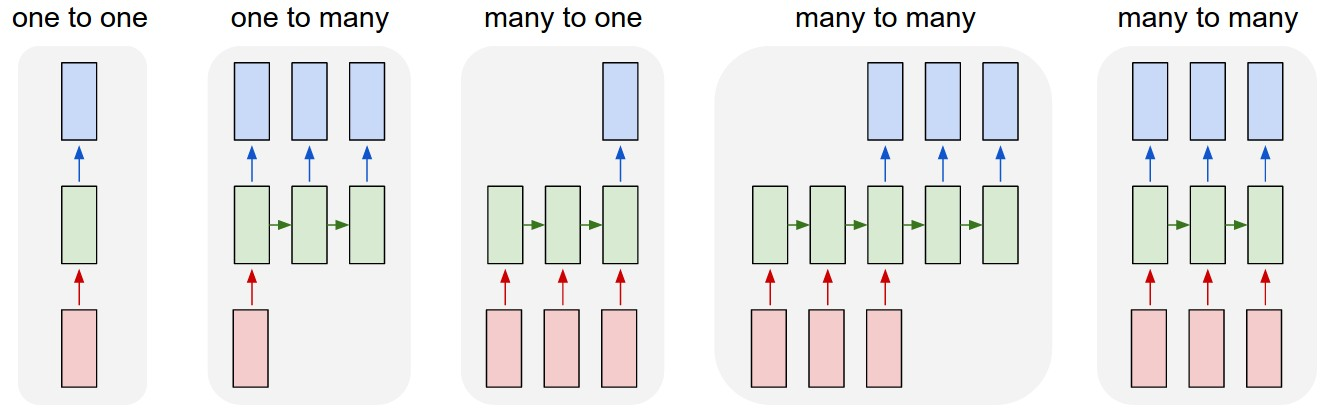
\includegraphics[width=1\textwidth]{rnnarch.jpg}
		\caption{Tipos de arquitecturas para una \textit{RNN}. \cite{karpathy:rnn}}
		\label{fig:rnnarch}
	\end{center}
\end{figure}

\textbf{\textit{One-to-one}}
Modo de procesamiento vanilla \textit{i.e.} sin \textit{RNN}, desde una entrada de tamaño fijo a una salida de tamaño fijo, por ejemplo la clasificación de imágenes.

\textbf{\textit{One-to-many}}

La entrada es un único dato y la salida es una secuencia. Un ejemplo de esta arquitectura es el "\textit{image captioning}" o subtitular imagen en donde la entrada es una y la salida es una secuencia de caracteres, un texto, que describe el contenido de la imagen.

\clearpage

\textbf{\textit{Many-to-one}}

La entrada es una secuencia y la salida es por ejemplo una categoría. Un ejemplo de esto es la clasificación de sentimientos, en donde por ejemplo la entrada es un texto que contiene una crítica a una película y la salida es una categoría indicando si la película le gustó a la persona o no.

\textbf{\textit{Many-to-many}}
Tanto la entrada como a la salida se tienen secuencias. La primer figura se refiere a \textit{RNN} utilizadas en traductores automáticos: en este caso la secuencia de salida no se genera al mismo tiempo que la secuencia de entrada pues para poder traducir por ejemplo una frase al español se requiere primero conocer la totalidad del texto en inglés. Y desde luego, en esta misma arquitectura podemos encontrar los conversores de voz a texto o texto a voz.
La segunda figura se refiere a secuencias sincronizadas de entrada y salida, por ejemplo clasificación de vídeo donde deseamos etiquetar cada fotograma.

Como era de esperar, el régimen secuencial de operación es mucho más poderoso en comparación con las redes fijas que están fijadas desde el principio por un número fijo de pasos computacionales y, por lo tanto, también es más provechoso a la hora de construir sistemas más inteligentes. 

Además, las \textit{RNN} combinan el vector de entrada con su vector de estado con una función fija (pero aprendida) para producir un nuevo vector de estado. En términos de programación, esto puede interpretarse como ejecutar un programa fijo con ciertas entradas y algunas variables internas. Visto de esta manera, los RNN esencialmente describen programas.

\textbf{Si entrenar redes neuronales es optimización sobre funciones, entrenar redes recurrentes es optimización sobre programas.}

\subsection{Funcionamiento}

Consideremos la figura~\ref{fig:rnnunit}, aquí podemos observar como se define de manera gráfica una unidad funcional de una \textit{RNN} denominada $A$, que toma una entrada $x_t$ y genera un valor $h_t$.

\begin{figure}[H]
	\begin{center}				
		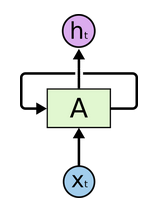
\includegraphics[width=0.17\textwidth]{tesis_27.png}
		\caption{Unidad funcional de \textit{RNN}. \citep{olahlstm}}
		\label{fig:rnnunit}
	\end{center}
\end{figure}

El \textit{loop} de A permite que la información pase de un paso de la red al siguiente.

Una red neuronal recurrente se puede considerar como múltiples copias de la misma red, cada una de las cuales pasa un mensaje a un sucesor. si desenrollamos el ciclo podemos representar la \textit{RNN} a través del eje del tiempo, como se muestra en la  figura~\ref{fig:rnnunrolled}.

\begin{figure}[H]
	\begin{center}
		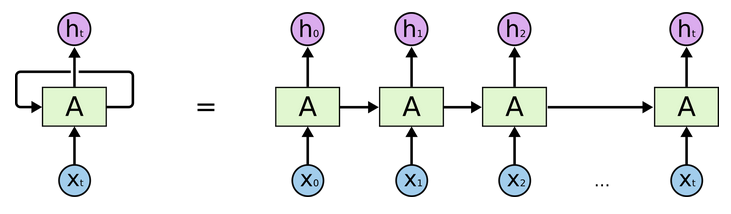
\includegraphics[width=0.9\textwidth]{tesis_28.png}
		\caption{Una \textit{RNN} desenrrollada. \citep{olahlstm}}
		\label{fig:rnnunrolled}
	\end{center}
\end{figure}

Esta naturaleza en cadena revela que las redes neuronales recurrentes están íntimamente relacionadas con secuencias y listas. En su esencia una \textit{RNN} se parece demasiado a una \textit{FFNN}, excepto que también tiene conexiones hacía atrás.

En la figura~\ref{fig:rnnunitv2} se observa que en cada instante de tiempo la red tiene realmente dos entradas y dos salidas. Las entradas son el dato actual, $x_t$ y la activación anterior, $a_{t-1}$, mientras que las salidas son la predicción actual, $y_t$, y la activación actual, $a_t$. Esta activación también recibe el nombre de \textit{hidden state} o estado oculto.

\begin{figure}[H]
	\begin{center}				
		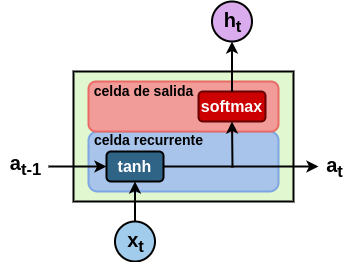
\includegraphics[width=0.5\textwidth]{rnnunitv2.png}
		\caption{Unidad funcional \textit{RNN} detallada. \citep{olahlstm}}
		\label{fig:rnnunitv2}
	\end{center}
\end{figure}

Se define:

$$ a_{t} = tanh(W_{aa}a_{t-1}+W_{ax}x_t+b_a) $$
$$ h_t = softmax(W_{ya}a_t + b_y) $$

Donde:

$ W_{ax}:$ matriz de pesos multiplicando la entrada.

$ W_{aa}:$ matriz de pesos multiplicando el estado oculto.

$ W_{ya}:$ matriz de pesos que relaciona el estado oculto a la salida.

$b_a:$ bias.

$b_y:$ bias que relaciona el estado oculto a la salida.

Es posible entrenar una \textit{RNN} con una gran cantidad de texto y le pediremos que modele la distribución de probabilidad del siguiente carácter en la secuencia dada una secuencia de caracteres anteriores. Esto nos permitirá generar texto nuevo, de a un carácter a la vez.

Como ejemplo práctico, suponga que solo tenemos un vocabulario de cuatro letras posibles \texttt{helo} y queremos entrenar a un \textit{RNN} en la secuencia de entrenamiento \texttt{hello}. 

Esta secuencia de entrenamiento es de hecho una fuente de 4 ejemplos de entrenamiento separados: 
\begin{enumerate}[noitemsep, topsep=2pt]
	\item La probabilidad de \texttt{e} probablemente debería estar dado el contexto de \texttt{h}.
	\item \texttt{l} debería estar probablemente en el contexto de \texttt{he}.
	\item \texttt{l} probablemente también debería ser dado el contexto de \texttt{hel}.
	\item  Y finalmente \texttt{o} debería ser probablemente dado el contexto de \texttt{hell}.
\end{enumerate}

Concretamente, codificaremos cada carácter en un vector usando la codificación \textit{1-of-k} (es decir, todo cero excepto uno en el índice del carácter en el vocabulario) y los introduciremos en el RNN uno a la vez con el función \texttt{step}. Luego observaremos una secuencia de vectores de salida de 4 dimensiones (una dimensión por carácter), que interpretamos como la confianza que el RNN asigna actualmente a cada carácter que sigue en la secuencia. 

\begin{figure}[H]
	\begin{center}				
		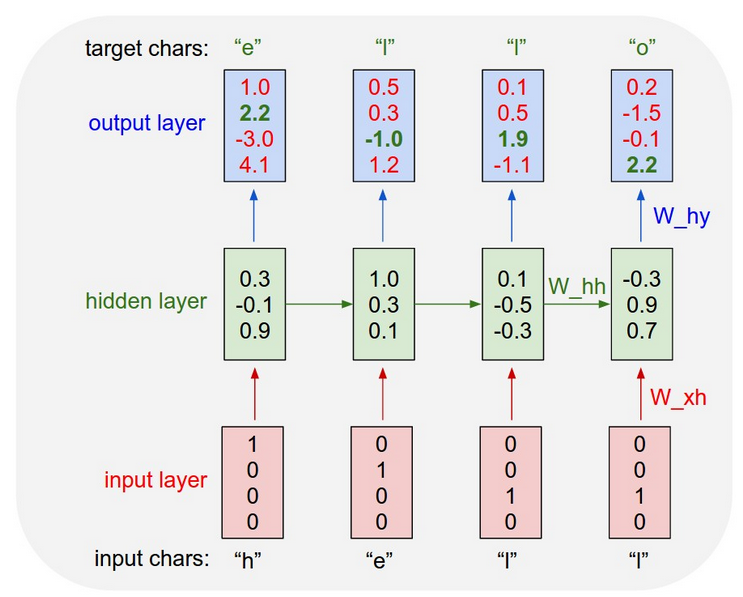
\includegraphics[width=0.6\textwidth]{tesis_29.png}
		\caption{Visualización del flujo de información a través de una \textit{RNN}. \citep{karpathy:rnn}}
		\label{fig:rnnexample}
	\end{center}
\end{figure}

En la Fig.~\ref{fig:rnnexample} observamos un ejemplo de \textit{RNN} con capas de entrada y salida de 4 dimensiones y una capa oculta de 3 unidades (neuronas). Las activaciones en el pase hacia adelante cuando el \textit{RNN} recibe los caracteres \texttt{"hell"} como entrada. La capa de salida contiene los pesos que el \textit{RNN} asigna al siguiente carácter (el vocabulario es \texttt{"h, e, l, o"}); Queremos que los números verdes sean altos y los números rojos bajos.

Por ejemplo, vemos que en el primer paso de tiempo cuando el \textit{RNN} vio el carácter \texttt{"h"} asignó un peso de $1.0$ a la siguiente letra que era \texttt{"h"}, $2.2$ a la letra \texttt{"e"}, $-3.0$ a \texttt{"l"} y $4.1$ a "o". 

Dado que en nuestros datos de entrenamiento (la cadena \texttt{"hello"}) el siguiente carácter correcto es \texttt{"e"}, nos gustaría aumentar su peso (verde) y disminuir los pesos de todas las demás letras (rojo). 

De manera similar, tenemos un carácter objetivo deseado en cada uno de los 4 pasos de tiempo a los que nos gustaría que la red le asignara una mayor confianza. Dado que el \textit{RNN} consta completamente de operaciones diferenciables, podemos ejecutar el algoritmo de \textit{back-propagation} para averiguar en qué dirección debemos ajustar cada uno de sus pesos para aumentar los pesos de los objetivos correctos. 

Luego podemos realizar una actualización de parámetros, que empuja cada peso una pequeña cantidad en esta dirección de gradiente. Si tuviéramos que alimentar las mismas entradas al RNN después de la actualización del parámetro, encontraríamos que las puntuaciones de los caracteres correctos (por ejemplo, "e" en el primer paso de tiempo) serían ligeramente más altas (por ejemplo, $2.3$ en lugar de $2.2$), y los pesos de los caracteres incorrectos serían ligeramente inferiores.

Luego, repetimos este proceso una y otra vez hasta que la red converge y sus predicciones son finalmente consistentes con los datos de entrenamiento en el sentido de que los caracteres correctos siempre se predicen a continuación.

\subsection{Entrenamiento}
Para entrenar una \textit{RNN}, el truco simplemente es desenrrollarla a través del tiempo y simplemente usar \textit{backpropagation} (estrategia que recibe el nombre de \textit{backpropagation} a través del tiempo (\textit{BPTT})) como observamos en la Fig.~\ref{fig:BPTT}.

\begin{figure}[H]
	\begin{center}				
		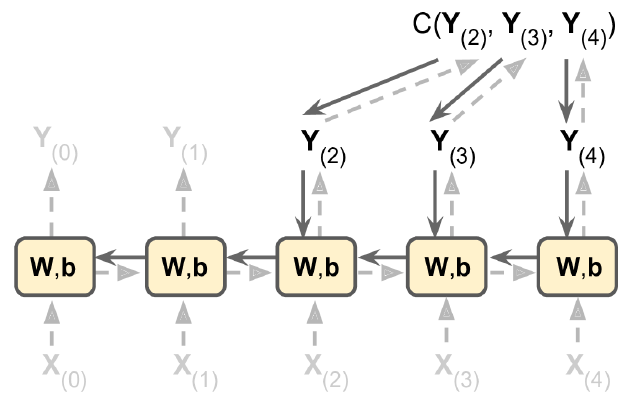
\includegraphics[width=0.6\textwidth]{tesis_40.png}
		\caption{\textit{Backpropagation} a través del tiempo.\citep{geron}}
		\label{fig:BPTT}
	\end{center}
\end{figure}

Primero realizamos una pasada hacía adelante a través de la red desenrollada (representada en la figura por las flechas punteadas). 

Luego la secuencia de salida es evaluada utilizando una función de costo $C(Y_{(0)}, Y_{(1)}, \dots, Y_{(T)})$ (donde $T$ es el paso máximo de tiempo). Notemos que la función de coste puede ignorar algunas salidas en función de lo que necesitemos como se muestra en la Fig.~\ref{fig:BPTT}.
Los gradientes de esa función de costo luego son propagados hacía atrás a través de la red desenrrollada (representada a través de las líneas sólidas).

Finalmente los parámetros del modelo son actualizadas usando los gradientes calculados por \textit{BPTT}. Notar que los gradientes fluyen hacía atrás a través de todas las salidas utilizadas por la función de costo, no solamente a través de la salida final (notar que en el ejemplo no fluye a través de $Y_{(0)}$ e $Y_{(1)}$).

\subsection{Desvanecimiento del gradiente}

Otra forma de alimentar una \textit{RNN} podría ser a través de las palabras individuales de una oración, dado que esto se realiza de forma secuencial, debemos proveerle de una palabra a la vez.

En el ejemplo de la Fig.~\ref{fig:rnnvanishing1} intentaremos predecir la intención del usuario tomando como entrada la oración \texttt{"What time is it?"}\citep{phi:rnn}.

\begin{figure}[H]
	\begin{center}				
		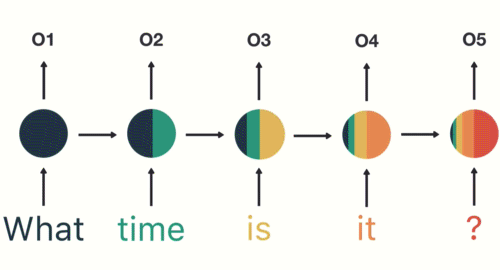
\includegraphics[width=0.5\textwidth]{vanishing1.png}
		\caption{\textit{RNN} siendo alimentada con las palabras de la oración. \citep{phi:rnn}}
		\label{fig:rnnvanishing1}
	\end{center}
\end{figure}

\begin{enumerate}[noitemsep, topsep=2pt]
	\item Inicializa sus capas de red y el estado oculto inicial. La forma y dimensión del estado oculto dependerá de la forma y dimensión de su \textit{RNN}.
	\item Luego recorre sus entradas, pasa la palabra y el estado oculto al \textit{RNN}.
	\item El \textit{RNN} devuelve la salida y un estado oculto modificado.
	\item Se repite hasta que quedar sin palabras.
	\item Por último, pasa la salida a la capa de \textit{feedforward} y devuelve una predicción (Fig.~\ref{fig:rnnvanishing2}).
\end{enumerate}

\begin{figure}[H]
	\begin{center}				
		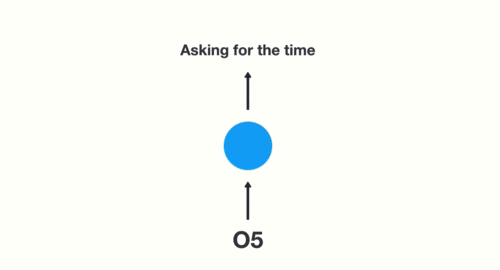
\includegraphics[width=0.6\textwidth]{vanishing2.png}
		\caption{Predicción de la \textit{RNN}.\citep{phi:rnn}}
		\label{fig:rnnvanishing2}
	\end{center}
\end{figure}

Pero prestemos atención a la Fig.~\ref{fig:rnnvanishing3}. Es posible que haya notado la irregular distribución de colores en los estados ocultos. Eso es para ilustrar un inconveniente con los \textit{RNN} conocido como memoria a corto plazo, causado por el problema del desvanecimiento del gradiente, que también prevalece en otras arquitecturas de redes neuronales. A medida que el RNN procesa más pasos, tiene problemas para retener información de los pasos anteriores.

\begin{figure}[H]
	\begin{center}				
		
\includegraphics[width=0.2\textwidth]{vanishin3.png}
		\caption{Estado oculto final de la \textit{RNN}.\citep{phi:rnn}}
		\label{fig:rnnvanishing3}
	\end{center}
\end{figure}

Como puede ver, la información de la palabra \texttt{"What"} y \texttt{"time"} es casi inexistente en el último paso. La memoria a corto plazo y el desvanecimiento del gradiente se deben a la naturaleza del algoritmo de \textit{back-propagation}.

Al hacer \textit{back-propagation}, cada nodo de una capa calcula su gradiente con respecto a los efectos de los gradientes, en la capa anterior. Entonces, si los ajustes a las capas anteriores son pequeños, los ajustes a la capa actual serán aún más pequeños. 

\begin{figure}[H]
	\begin{center}				
		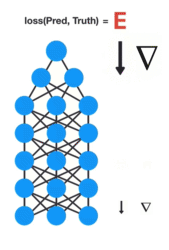
\includegraphics[width=0.25\textwidth]{vanishing4.png}
		\caption{Desvanecimiento del gradiente desde las capas superiores a las inferiores.}
		\label{fig:rnnvanishing4}
	\end{center}
\end{figure}

Es posible pensar en cada paso de tiempo en una \textit{RNN} como una capa y para entrenarla se usa \textit{back-propagation} a través del tiempo. Los valores del gradiente se reducirán exponencialmente a medida que se propaga a través de cada paso de tiempo.

\begin{figure}[H]
	\begin{center}				
		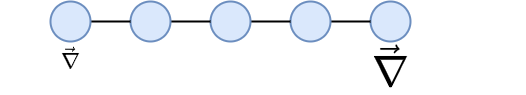
\includegraphics[width=0.6\textwidth]{vanishing5.png}
		\caption{El gradiente se achica a medida que se propaga hacia atrás en el tiempo.}
		\label{fig:rnnvanishing5}
	\end{center}
\end{figure}

Nuevamente, el gradiente se utiliza para realizar ajustes en los pesos de las redes neuronales, lo que le permite aprender. Pequeños gradientes significan pequeños ajustes. Eso hace que las capas tempranas no aprendan.

Debido a los gradientes que desaparecen, la \textit{RNN} no aprende las dependencias de largo alcance en los pasos de tiempo. Eso significa que existe la posibilidad de que las palabras \texttt{"What"} y \texttt{"time"} no se consideren al intentar predecir la intención del usuario. Entonces, la red tiene que hacer la mejor suposición con \texttt{"is it?"}. Eso es bastante ambiguo y sería difícil incluso para un humano. Por lo tanto, no poder aprender en pasos de tiempo anteriores hace que la red tenga una memoria a corto plazo.

\subsection{Tipos de \textit{RNNs}}
Para mitigar la memoria a corto plazo, se crearon dos redes neuronales recurrentes especializadas. Las redes denominadas \textit{Long Short-Term Memory} o \textit{LSTM} para abreviar. Las otras se denominan \textit{Gated Recurrent Units} o \texttt{GRU}.

\subsubsection{LSTM}
Los \texttt{LSTM} y \texttt{GRU} funcionan esencialmente como los \textit{RNN}, pero son capaces de aprender las dependencias a largo plazo mediante mecanismos llamados "puertas". Estas puertas son diferentes operaciones de tensor que pueden aprender qué información agregar o quitar al estado oculto. Debido a esta capacidad, la memoria a corto plazo es un problema menor para ellos. \citep{olahlstm}

Si consideramos la celda \texttt{LSTM} como una caja negra, aparenta ser idéntica a una \textit{RNN} excepto que su estado se divide en dos vectores: $h_{(t)}$ y $c_{(t)}$ ("c" se mantiene por celda). Es posible pensar a $h_{(t)}$ como un estado de corto plazo y a $c_{(t)}$ como un estado de largo plazo.

El diagrama completo del \texttt{LSTM} lo podemos observar en la Fig.\ref{fig:lstmcell}, pero vamos a ir paso a paso analizando cada una de las partes que lo componen.

\begin{figure}[H]
	\begin{center}				
		\includegraphics[width=0.95\textwidth]{lstmcell5.png}
		\caption{Celda \texttt{LSTM}.}
		\label{fig:lstmcell}
	\end{center}
\end{figure}

La clave de los \texttt{LSTM} es el estado de la celda, la línea horizontal que atraviesa la parte superior de la Fig.~\ref{fig:lstm1}. El estado de la celda es como una cinta transportadora. Corre directamente a lo largo de toda la cadena, con solo algunas interacciones lineales menores. Es muy fácil que la información fluya sin cambios.

\begin{figure}[H]
	\begin{center}				
		\includegraphics[width=1\textwidth]{lstm1.png}
		\caption{Celda de estado. \citep{olahlstm}}
		\label{fig:lstm1}
	\end{center}
\end{figure}

El \texttt{LSTM} tiene la capacidad de eliminar o agregar información al estado de la celda, regulada cuidadosamente por estructuras llamadas puertas. Las puertas son una forma de dejar pasar información opcionalmente. Están compuestos por una capa de red neuronal sigmoidea y una operación de multiplicación.

La capa sigmoidea genera números entre $0$ y $1$, que describen cuánto de cada componente debe dejarse pasar. Un valor de $0$ significa "no dejar pasar nada", mientras que un valor de $1$ significa "dejar pasar todo". Un \texttt{LSTM} tiene tres de estas puertas para proteger y controlar el estado de la celda.

El primer paso es decidir qué información vamos a eliminar del estado de la celda. Esta decisión la toma una capa sigmoidea llamada \textbf{puerta del olvido} (Fig.~\ref{fig:lstm2}). Examina $h_{t-1}$ y $x_t$, y genera un número entre $0$ y $1$ para cada número en el estado de celda $C_{t-1}$. Un $1$ representa "mantener esto completamente", mientras que un $0$ representa "deshacerse de esto por completo".

\begin{figure}[H]
	\begin{center}				
		\includegraphics[width=0.5\textwidth]{lstm2.png}
		\caption{Puerta del olvido. \citep{olahlstm}}
		\label{fig:lstm2}
	\end{center}
\end{figure}

Por tanto la puerta del olvido queda representada por la siguiente ecuación:

$$f_{(t)} = \sigma (W_{xf}x_{(t)} + W_{hf}h_{(t-1)} + b_f)$$

El siguiente paso es decidir qué nueva información almacenaremos en el estado de la celda. Esto tiene dos partes. 

\begin{figure}[H]
	\begin{center}				
		\includegraphics[width=0.5\textwidth]{lstm3.png}
		\caption{Puerta de entrada. \citep{olahlstm}}
		\label{fig:lstm3}
	\end{center}
\end{figure}

Una capa sigmoidea llamada \textbf{puerta de entrada} (Fig~\ref{fig:lstm3}) decide qué valores actualizaremos.

$$i_{(t)}=\sigma(W_{xi}x_{(t)} + W_{hi}h_{(t-1)} + b_i)$$

A continuación, una capa $tanh$ crea un vector de nuevos valores candidatos, que podrían agregarse al estado. 

$$g_{(t)}=tanh(W_{xg}x_{(t)}+W_{hg}h_{(t-1)}+b_g)$$


En el siguiente paso, combinaremos estos dos para crear una actualización del estado.

Ahora es el momento de actualizar el estado de la celda anterior, $C_{(t-1)}$, al nuevo estado de la celda $C_{(t)}$. Los pasos anteriores ya decidieron qué hacer, solo tenemos que hacerlo realmente.

\begin{figure}[H]
	\begin{center}				
		\includegraphics[width=0.5\textwidth]{lstm4.png}
		\caption{Actualización de la celda. \citep{olahlstm}}
		\label{fig:lstm4}
	\end{center}
\end{figure}

Multiplicamos el estado anterior por $f_{(t)}$, olvidando las cosas que decidimos olvidar antes. Luego le sumamos $i_{(t)} \otimes g_{(t)}$. Estos son los nuevos valores candidatos, escalados según cuánto decidimos actualizar cada valor de estado.

$$C_{(t)} = f_{(t)} \otimes C_{(t-1)} + i_{(t)} \otimes g_{(t)}$$

\begin{figure}[H]
	\begin{center}				
		\includegraphics[width=0.5\textwidth]{lstm5.png}
		\caption{Puerta de salida. \citep{olahlstm}}
		\label{fig:lstm5}
	\end{center}
\end{figure}

Finalmente, tenemos que decidir qué vamos a producir. Esta salida se basará en el estado de nuestra celda, pero será una versión filtrada. Primero, ejecutamos una capa sigmoidea que denominaremos \textbf{puerta de salida} que decide qué partes del estado de la celda vamos a generar. Luego, colocamos el estado de la celda a través de $tanh$ (para presionar los valores entre $-1$ y $1$) y lo multiplicamos por la salida de la puerta, de modo que solo produzcamos las partes que decidimos.

$$ o_{(t)}=\sigma (W_{xo}x_{(t)} + W_{ho}h_{(t-1)} + b_o) $$

$$ h_{(t)}=o_{(t)} \otimes tanh(C_{(t)})$$

Pasando en limpio observando nuevamente la Fig.~\ref{fig:lstmcell}, tendremos nuestro vector de entradas $x_{(t)}$ y el estado anterior de corto plazo $h_{(t-1)}$ que alimenta 4 capas \texttt{FC}. Cada una de ellas sirve a un propósito diferente \citep{geron}:

\begin{itemize}[noitemsep, topsep=2pt]
	\item La capa principal es la que genera $g_{(t)}$. Tiene la función habitual de analizar las entradas actuales $x_{(t)}$ y el estado anterior (a corto plazo) $h_{(t-1)}$. En una celda básica \textit{RNN}, no hay nada más que esta capa, y su salida va directamente hacia $y_{(t)}$ y $h_{(t)}$. Por el contrario, en una celda \texttt{LSTM}, la salida de esta capa no sale directamente, sino que se almacena parcialmente en el estado a largo plazo.
	\item Las otras tres capas son controladores de puerta. Dado que usan la función de activación sigmoidea, sus salidas van entre 0 y 1. Sus salidas se alimentan a operaciones de multiplicación elemento a elemento (también conocido como producto de Hadamard \citep{hadamard}), por lo que si generan ceros, cierran la puerta, y si generan 1 la abre. Específicamente:
	      \begin{itemize}[noitemsep, topsep=2pt]
	      	\item La puerta de olvido (controlada por $f_{(t)}$) controla qué partes del estado a largo plazo $C_{(t-1)}$ deben borrarse.
	      	\item La puerta de entrada (controlada por $i_{(t)}$) controla qué partes de $g_{(t)}$ deben agregarse al estado a largo plazo.
	      	\item La puerta de salida (controlada por $o_{(t)}$) controla qué partes del estado a largo plazo deben leerse y generarse en este paso de tiempo (tanto en $h_{(t)}$ como en $y_{(t)}$).
	      \end{itemize}
\end{itemize}

En resumen, una celda \texttt{LSTM} puede aprender a reconocer una entrada importante (puerta de entrada), almacenarla en el estado a largo plazo, aprender a preservarla durante el tiempo que sea necesario (puerta del olvido) y aprender a extraerla siempre que sea necesario (puerta de salida).

\subsubsection{GRU}

Otra variante popular es la celda \texttt{GRU} (Unidad Recurrente Cerrada, \textit{Gated Recurrent Unit)}. \citep{olahlstm}

\begin{figure}[H]
	\begin{center}				
		\includegraphics[width=0.5\textwidth]{gru2.png}
		\caption{Celda \texttt{GRU}. \citep{olahlstm}}
		\label{fig:lstm5}
	\end{center}
\end{figure}

Hace algunas simplificaciones \citep{geron}:

\begin{itemize}[noitemsep, topsep=2pt]
	\item Ambos vectores de estado son combinados en un único vector $h_{(t)}$.
	\item Un controlador de puerta única $z_{(t)}$ controla tanto la puerta de olvido como la puerta de entrada. Si el controlador de puerta genera un 1, la puerta de olvido está abierta $(=1)$ y la puerta de entrada está cerrada $(1-1=0)$. Si genera un 0, sucede lo contrario. En otras palabras, siempre que se deba almacenar una memoria, primero se borra la ubicación donde se almacenará.
	\item No hay puerta de salida; el vector de estado completo se genera en cada paso de tiempo. Sin embargo, hay un nuevo controlador de puerta $r_{(t)}$ que controla qué parte del estado anterior se mostrará en la capa principal $g_{(t)}$.
	      	      	      
\end{itemize}

Las ecuaciones quedan de la siguiente forma:

$$z_{(t)}=\sigma(W_{xz}x_{(t)} + W_{hx}h_{(t-1)} + b_z)$$
$$r_{(t)}=\sigma(W_{xr}x_{(t)} + W_{hr}h_{(t-1)} + b_r)$$
$$g_{(t)}=\sigma(W_{xg}x_{(t)} + W_{hg}h_{(t-1)} + b_g)$$
$$h_{(t)}=z_{(t)} \otimes h_{(t-1)} + (1-z_{(t)}) \otimes g_{(t)}$$

\subsection{Secuencias de entradas y salida}

Si bien en la Sección~\ref{rnnarchitecture} ya desglosamos los diferentes tipos de arquitecturas que puede tener una \textit{RNN}, sería de utilidad ahora que ya poseemos un marco teórico aceptable describirlas un poco más y ejemplificar en que casos sería provechosa su utilización. Tomaremos como referencia la figura~\ref{fig:rnnnets}.

\begin{figure}[H]
	\begin{center}				
		\includegraphics[width=0.80\textwidth]{tesis_42.png}
		\caption{\textbf{Superior-izquierda}: \textit{seq-to-seq}. \textbf{Superior-derecha}: \textit{sec-to-vector}. \textbf{Inferior-izquierda}: \textit{vector-to-sec}. \textbf{Inferior-derecha}: \textit{encoder-decoder}. \citep{geron}}
		\label{fig:rnnnets}
	\end{center}
\end{figure}

\textbf{Secuencia a secuencia}

Una \textit{RNN} puede tomar simultáneamente una secuencia de entradas y producir una secuencia de salidas (red \textbf{superior-izquierda}). Por ejemplo, este tipo de red es útil para predecir series de tiempo como los precios de las acciones: usted le da los precios de los últimos $N$ días y debe generar los precios desplazados un día en el futuro (es decir, de $N - 1$ días hace hasta mañana).

\textbf{Secuencia a vector}

Alternativamente, puede alimentar a la red con una secuencia de entradas e ignorar todas las salidas excepto la última (red \textbf{superior-derecha}). En otras palabras, esta es una red de secuencia a vector. Por ejemplo, podría alimentar a la red con una secuencia de palabras correspondiente a una crítica de película y la red generaría una puntuación de sentimiento (\textit{e.g.}, de 0 [odio] a 1 [amor]).

\textbf{Vector a secuencia}

Por el contrario, puede alimentar la red con una sola entrada en el primer paso de tiempo (y ceros para todos los demás pasos de tiempo) y dejar que genere una secuencia (red \textbf{inferior-izquierda}). Por ejemplo, la entrada podría ser una imagen y la salida podría ser un título para esa imagen.

\textbf{Secuencia a secuencia con retardo}

Por último, podría tener una red de secuencia a vector, llamada \textit{encoder}, seguida de una red de vector a secuencia, llamada \textit{decoder} (consulte la red de la parte inferior derecha). Por ejemplo, esto se puede utilizar para traducir una oración de un idioma a otro. Alimentaría la red con una oración en un idioma, el \textit{encoder} convertiría esta oración en una representación de vector único y luego el \textit{decoder} decodificaría este vector en una oración en otro idioma. Este modelo de dos pasos, llamado \textit{encoder-decoder}, funciona mucho mejor que intentar traducir sobre la marcha con un único \textit{RNN} secuencia a secuencia (red \textbf{Superior-izquierda}), ya que las últimas palabras de una oración pueden afectan las primeras palabras de la traducción, por lo que debe esperar hasta que haya escuchado la oración completa antes de traducirla.

\clearpage
\section{Optimización de hiperparámetros} \label{tuning-hp}
Los parámetros que definen la arquitectura del modelo se denominan hiperparámetros y, por lo tanto, este proceso de búsqueda de la arquitectura del modelo ideal se denomina ajuste de hiperparámetros o \textit{hyperparameters tuning}. \citep{Koehrsen2018Jul}

Los hiperparámetros no son parámetros del modelo y no se pueden entrenar directamente a partir de los datos. Mientras que los parámetros del modelo especifican cómo transformar los datos de entrada en la salida deseada a través del entrenamiento optimizando una función de pérdida, los hiperparámetros definen cómo está realmente estructurado nuestro modelo.

Los métodos de ajuste de hiperparámetros se relacionan con cómo muestreamos posibles candidatos a la arquitectura del modelo a partir del espacio de posibles valores de hiperparámetros. Esto se denomina a menudo "buscar" en el espacio de hiperparámetros los valores óptimos.

En general, este proceso incluye:

\begin{enumerate}[noitemsep, topsep=2pt]
	\item Definir los modelos.
	\item Definir el rango de valores posibles para todos los hiperparámetros, es decir el espacio de búsqueda o \textit{search space}.
	\item Definir un algoritmo para obtener valores de hiperparámetros.
	\item Definir un criterio evaluativo para juzgar el modelo.
\end{enumerate}

La optimización de hiperparámetros se representa en forma de ecuación como:

$$x^* = \operatorname*{argmin}_{x \in X} f(x)$$

Aquí $f(x)$ representa una puntuación objetivo para minimizar (usualmente una métrica), evaluada en el set de validación; $x^*$ es el conjunto de hiperparámetros que produce el menor valor para la función objetivo, y $x$ puede tomar cualquier valor en el dominio $X$. En términos simples, queremos encontrar los hiperparámetros del modelo que producen la mejor puntuación en la métrica del conjunto de validación.

El problema con la optimización de hiperparámetros es que evaluar la función objetivo para encontrar la puntuación es extremadamente costoso. Cada vez que probamos diferentes hiperparámetros, tenemos que entrenar un modelo con los datos de entrenamiento, hacer predicciones sobre los datos de validación y luego calcular la métrica de validación. Con una gran cantidad de hiperparámetros y modelos complejos, como conjuntos o redes neuronales profundas que pueden tardar días en entrenarse, y el problema no escala.

\subsection{Algoritmos} \label{algo-hp}

Los algoritmos de optimización de hiperparámetros se pueden dividir en tres categorías principales:
\begin{itemize}[noitemsep, topsep=2pt]
	\item \textbf{Búsqueda exhaustiva del espacio}: estos métodos son una primera opción atractiva para la optimización, ya que son muy fáciles de codificar, se pueden ejecutar en paralelo y no necesitan ningún tipo de ajuste. Su inconveniente es que no hay garantía de encontrar un mínimo local con cierta precisión, excepto si el espacio de búsqueda se muestrea a fondo. Esto no supone ningún problema si el modelo es muy rápido de ejecutar y el número de hiperparámetros es bajo. Si el modelo tarda mucho en ejecutarse utilizando una gran cantidad de recursos computacionales estos métodos son ineficaces, ya que no utilizan la información obtenida de todos los intentos anteriores.
	\item \textbf{Modelos subrogados:} un modelo subrogado de la función de hiperparámetros puede ajustarse a los intentos anteriores y decir dónde podría estar el mínimo local. Estos métodos se denominan optimización basada en modelos secuenciales (SMBO, \textit{Sequential Model-Based Optimization}).
	\item \textbf{Reducciones sucesivas a la mitad:} son algoritmos que se encargan de seleccionar dos configuraciones de hiperparámetros e irlas descartando tempranamente para así converger a la mejor.
\end{itemize}

Para todos los algoritmos, se debe definir un espacio de búsqueda de antemano para así establecer límites para todos los hiperparámetros.

\subsubsection{Búsqueda exhaustiva del espacio}
\textbf{Búsqueda por grilla (\textit{Grid search})}

El espacio de búsqueda de cada hiperparámetro se discretiza, y el espacio de búsqueda total se discretiza como los productos cartesianos de ellos. Luego, el algoritmo lanza un aprendizaje para cada una de las configuraciones de hiperparámetros y selecciona la mejor al final. Es un problema paralelo (siempre que uno tenga la potencia de cálculo necesaria para entrenar varios modelos al mismo tiempo) pero sufre el problema de la dimensionalidad (el número de configuraciones a probar es exponencial con respecto al número de hiperparámetros a ser optimizado).

\textbf{Búsqueda aleatoria (\textit{Random search})}
Una variación del algoritmo anterior, que muestrea aleatoriamente el espacio de búsqueda en lugar de discretizarlo con una cuadrícula cartesiana. El algoritmo no tiene fin. En su lugar, se debe especificar un presupuesto de tiempo (en otras palabras, una número de \textit{trials} o pruebas). 

Este algoritmo también sufre el problema de la dimensionalidad para alcanzar una densidad de muestreo fija preestablecida. Una de las ventajas de la búsqueda aleatoria es que si dos hiperparámetros están poco correlacionados, la búsqueda aleatoria permite encontrar con mayor precisión los óptimos de cada parámetro, como se muestra en la fig.~\ref{fig:grid_vs_search}. 

\begin{figure}[H]
	\begin{center}
		\includegraphics[width=1\textwidth]{grid_vs_search_v4.png}
		\caption{Comparación de \textit{Grid Search} vs \textit{Random Search}.}
		\label{fig:grid_vs_search}
	\end{center}
\end{figure}

\subsubsection{Modelos subrogados}

\textbf{Optimización bayesiana (\textit{Bayesian Optimization})} 

Tenemos una función $f(x)$, que es costosa de calcular, no es necesariamente una expresión analítica y no conoce su derivada. Y nuestro objetivo es encontrar los mínimos globales. \citep{Ye2020Oct}

Esta es sin duda una tarea difícil, más incluso que otros problemas de optimización dentro del aprendizaje automático. El descenso de gradiente, por ejemplo, tiene acceso a las derivadas de una función y aprovecha los atajos matemáticos para una evaluación de expresiones más rápida.

Alternativamente, en algunos escenarios de optimización, la función es simple de evaluar. Si podemos obtener cientos de resultados para variantes de una entrada $x$ en unos pocos segundos, se puede emplear una simple \textit{grid search} con buenos resultados.

Desafortunadamente, no contamos con estas bondades y estamos limitados en nuestra optimización por varios frentes, en particular:
\begin{itemize}[noitemsep, topsep=2pt]
	\item \textbf{Es costoso de calcular}. Idealmente, podríamos consultar la función lo suficiente como para replicarla, pero nuestro método de optimización debe funcionar con una muestra limitada de entradas.
	\item \textbf{Se desconoce la derivada}. Por tanto no podemos aplicar el descenso del gradiente y sus derivados.
	\item \textbf{Necesitamos encontrar los mínimos globales}. Esta es una tarea difícil incluso para un método sofisticado como el descenso de gradiente, entonces nuestro modelo de alguna manera necesitará un mecanismo para evitar quedar atrapado en los mínimos locales.
\end{itemize}

La solución es \textbf{optimización bayesiana} (\textit{Bayesian Optimization}), que proporciona un marco elegante para abordar problemas que se asemejan al escenario descrito para encontrar el mínimo global en el menor número de pasos.

Construyamos un ejemplo hipotético de la función objetivo $c(x)$, o el costo de un modelo dado una entrada $x$. Por supuesto, el aspecto de la función estará oculto al optimizador; la verdadera forma de $c(x)$ es la de la fig~\ref{fig:cx}.

\begin{figure}[H]
	\begin{center}
		\includegraphics[width=0.7\textwidth]{bayes_opt_1_v2.png}
		\caption{Representación gráfica de la función $c(x)$.}
		\label{fig:cx}
	\end{center}
\end{figure}

La optimización bayesiana aborda esta tarea mediante un método conocido como optimización subrogada. Por contexto, una maternidad subrogada es la práctica por la que, previo acuerdo con otra persona, una mujer se queda embarazada, lleva la gestación a término y da a luz a un bebé para esa otra persona o pareja \citep{vientre_alquiler}; en ese contexto, una función subrogada es una aproximación de la función objetivo y se forma sobre la base de puntos muestreados tal como muestra la fig.~\ref{fig:bayes2}.

\begin{figure}[H]
	\begin{center}
		\includegraphics[width=0.8\textwidth]{bayes_opt_2_v2.png}
		\caption{Función subrogada.}
		\label{fig:bayes2}
	\end{center}
\end{figure}

Basándonos en la función subrogada, podemos identificar qué puntos son mínimos prometedores. Decidimos tomar más muestras de estas regiones prometedoras y actualizar la función subrogada en consecuencia (fig.~\ref{fig:bayes3}).

\begin{figure}[H]
	\begin{center}
		\includegraphics[width=0.8\textwidth]{bayes_opt_3_v2.png}
		\caption{Actualización de función subrogada.}
		\label{fig:bayes3}
	\end{center}
\end{figure}

En cada iteración, continuamos examinando la función subrogada actual, aprendemos más sobre las áreas de interés mediante el muestreo y actualizamos la función. Tenga en cuenta que la función subrogada se expresará matemáticamente de una manera significativamente menos costosa de evaluar (por ejemplo, $y=x$ es una aproximación de una función más costosa, $y = arcsin \left( \frac{1-cos^2x}{sen x} \right)$ dentro de un cierto rango).

Después de un cierto número de iteraciones, estamos destinados a llegar a un mínimo global, a menos que la forma de la función sea muy irregular (en el sentido de que tiene grandes oscilaciones hacia arriba y hacia abajo) por tanto se debería hacer más foco sobre los datos que en la optimización.

Este enfoque no hace ninguna suposición sobre la función (excepto que es optimizable en primer lugar), no requiere información sobre derivadas y es capaz de utilizar el razonamiento de sentido común mediante el uso ingenioso de una función de aproximación continuamente actualizada. La costosa evaluación de nuestra función objetivo original no es un problema en absoluto.

La esencia de los modelos bayesianos es la actualización de una creencia previa ("antes") utilizando nueva información para producir una creencia posterior ("después") actualizada. Esto es exactamente lo que hace la optimización subrogada en este caso, por lo que se puede representar mejor a través de sistemas, fórmulas e ideas bayesianos.

La función subrogada generalmente está representada por \textbf{procesos gaussianos}, que se puede considerar como una tirada de dados que devuelve funciones ajustadas a puntos de datos dados (por ejemplo, $sin$, $log$) en lugar de números del 1 al 6 (fig.~\ref{fig:bayes4}). El proceso devuelve varias funciones, que tienen probabilidades asociadas.

\begin{figure}[H]
	\begin{center}
		\includegraphics[width=0.8\textwidth]{bayes_opt_4.png}
		\caption{Varias funciones generadas por procesos gaussianos para cuatro puntos de datos. \citep{Ye2020Oct}}
		\label{fig:bayes4}
	\end{center}
\end{figure}

\begin{figure}[H]
	\begin{center}
		\includegraphics[width=0.8\textwidth]{bayes_opt_5.png}
		\caption{Las funciones agregadas. \citep{Ye2020Oct}}
		\label{fig:bayes5}
	\end{center}
\end{figure}

Hay una buena razón por la que se utilizan procesos gaussianos, y no algún otro método de ajuste de curvas, para modelar la función subrogada: es de naturaleza bayesiana. Un proceso gaussiano es una distribución de probabilidad, como una distribución de los resultados finales de un evento (por ejemplo, 1/2 probabilidad de lanzar una moneda), pero sobre todas las funciones posibles.

Por ejemplo, podemos definir el conjunto actual de puntos de datos como 40\% representable por la función $a(x)$, 10\% por la función $b(x)$, etc. Al representar la función sustituta como una distribución de probabilidad, se puede actualizar con nueva información a través de procesos bayesianos intrínsecamente probabilísticos. Quizás cuando se introduce nueva información, los datos solo son representables en un 20\% por la función $a(x)$. Estos cambios se rigen por fórmulas bayesianas.

La función subrogada, representada como una distribución de probabilidad se actualiza con una \textbf{función de adquisición}. Esta función es responsable de impulsar la propuesta de nuevos puntos para probar, en una compensación de exploración y explotación:
\begin{itemize}[noitemsep, topsep=2pt]
	\item \textbf{Explotación:} busca muestrear dónde el modelo subrogada predice un buen objetivo. Esto está aprovechando los lugares prometedores conocidos. Sin embargo, si ya hemos explorado una determinada región lo suficiente, la explotación continua de información conocida producirá poca ganancia.
	\item \textbf{Exploración}: busca muestrear en lugares donde la incertidumbre es alta. Esto asegura que no quede ninguna región importante del espacio sin explorar; es posible que los mínimos globales se encuentren allí.
\end{itemize}

Una función de adquisición que fomente demasiada explotación y muy poca exploración hará que el modelo resida solo un mínimo que encuentre primero (generalmente local). Una función de adquisición que fomente lo contrario no se quedará en mínimos, locales o globales, en primer lugar. Dando buenos resultados en un delicado equilibrio.

La función de adquisición, que denotaremos $a(x)$, debe considerar tanto la explotación como la exploración. Las funciones de adquisición comunes incluyen la mejora esperada y la probabilidad máxima de mejora, todas las cuales miden la probabilidad de que una entrada específica pueda dar resultados en el futuro, dada la información sobre el anterior (el proceso gaussiano). Existen diversas funciones de adquisición tales como \textit{Upper Confidence Bound (UCB)}, \textit{Probability of Improvement (PI)}, \textit{Expected Improvement (EI)}, etc. \citep{Agnihotri2020May}

Juntemos las piezas. La optimización bayesiana se puede realizar como tal:
\begin{enumerate}[noitemsep, topsep=2pt]
	\item Inicializar una distribución previa de función subrogada del proceso gaussiano.
	\item Elija varios puntos de datos $x$ de modo que se maximice la función de adquisición $a(x)$ que opera en la distribución anterior actual.
	\item Evalúe los puntos de datos $x$ en la función de costo objetivo $c(x)$ y obtenga los resultados, $y$.
	\item Actualice la distribución previa del proceso gaussiano con los nuevos datos para producir un posterior (que se convertirá en el anterior en el siguiente paso).
	\item Repita los pasos 2 a 5 para varias iteraciones.
	\item Interprete la distribución actual del proceso gaussiano (que es poco costoso de realizar) para encontrar los mínimos globales.
\end{enumerate}

La optimización bayesiana se trata de poner ideas probabilísticas detrás de la idea de optimización subrogada. La combinación de estas dos ideas crea un sistema poderoso con muchas aplicaciones, desde el desarrollo de productos farmacéuticos hasta vehículos autónomos. Sin embargo, más comúnmente en el aprendizaje automático, la optimización bayesiana se usa para la optimización de hiperparámetros. Por ejemplo, si estamos entrenando un clasificador de aumento de gradiente, hay docenas de parámetros, desde la tasa de aprendizaje hasta la profundidad máxima de capas de la red, la cantidad de neuronas de cada capa entre otras por nombrar algunos ejemplos. En este caso, $x$ representa los hiperparámetros del modelo y $c(x)$ representa el rendimiento del modelo.

\clearpage

La principal motivación para utilizar la optimización bayesiana se encuentra en escenarios en los que es muy costoso evaluar la salida, tal como el entrenamiento de múltiples arquitecturas de modelos para encontrar la mejor.

Para dejar clara la idea:

\begin{itemize}[noitemsep, topsep=2pt]
	\item La optimización subrogada utiliza una función subrogada o aproximada para estimar la función objetivo a través del muestreo.
	\item La optimización bayesiana coloca la optimización sustituta en un marco probabilístico al representar funciones sustitutas como distribuciones de probabilidad, que pueden actualizarse al obtener nueva información.
	\item Las funciones de adquisición se utilizan para evaluar la probabilidad de que la exploración de un determinado punto en el espacio produzca un rendimiento "bueno" dado lo que se conoce actualmente de la exploración y la explotación anteriores, equilibrando la exploración.
	\item Utilice la optimización bayesiana principalmente cuando la función objetivo sea costosa de evaluar, comúnmente utilizada en el ajuste de hiperparámetros.
\end{itemize}

Ahora extrapolemos el conocimiento adquirido al ajuste de hiperparámetros teniendo en cuenta que la optimización bayesiana crea un modelo de probabilidad de la función objetivo. \citep{Wang2020Apr}

La función objetivo real es una función fija. Supongamos que se parece a la figura~\ref{fig:bayes6}, pero obviamente desconocemos su forma.

\begin{figure}[H]
	\begin{center}
		\includegraphics[width=0.7\textwidth]{bayes_opt_6_v2.png}
		\caption{Función objetivo real.}
		\label{fig:bayes6}
	\end{center}
\end{figure}

Dado que calcular la métrica de nuestro modelo es costoso, digamos que solo tenemos 10 muestras, representada como círculos negros en la figura~\ref{fig:bayes7}.

\begin{figure}[H]
	\begin{center}
		\includegraphics[width=0.7\textwidth]{bayes_opt_7_v2.png}
		\caption{Muestras de la función objetivo real.}
		\label{fig:bayes7}
	\end{center}
\end{figure}

Usando estas 10 muestras, necesitamos construir un modelo subrogado (también llamado modelo de superficie de respuesta) para aproximarnos a la función objetivo real. Observemos la fig.~\ref{fig:bayes8}, el modelo subrogado se representa como la línea azul y la sombra azul representa la desviación.

\begin{figure}[H]
	\begin{center}
		\includegraphics[width=0.7\textwidth]{bayes_opt_8_v2.png}
		\caption{Modelo subrogado.}
		\label{fig:bayes8}
	\end{center}
\end{figure}

Un modelo (o función) subrogado es un modelo probabilístico que asigna hiperparámetros a una probabilidad de la puntuación de una métrica en la función objetivo real. Entonces queda formalmente definido como:

$$ P(y|x) $$

Dónde $y$ representa la puntuación de la métrica y $x$ el conjunto de hiperparámetros seleccionado.

Ahora tenemos 10 muestras de la función objetivo, para decidir qué parámetro probar como la undécima muestra necesitamos construir la función de adquisición. El siguiente hiperparámetro de elección es donde se maximiza la función de adquisición.

En la fig.~\ref{fig:bayes9} abajo, el tono verde es la función de adquisición y la línea recta roja es donde se maximiza. Por lo tanto, el hiperparámetro correspondiente y su puntuación de función objetivo, representada como un círculo rojo, se utiliza como la undécima muestra para actualizar el modelo subrogado (fig.~\ref{fig:bayes9} arriba).

\begin{figure}[H]
	\begin{center}
		\includegraphics[width=0.7\textwidth]{bayes_opt_9_v2.png}
		\caption{\textbf{Arriba}: modelo subrogado. \textbf{Abajo:} función de adquisición.}
		\label{fig:bayes9}
	\end{center}
\end{figure}

Luego de usar una función de adquisición para determinar el siguiente hiperparámetro, se obtiene la puntuación de la función objetiva real de este nuevo hiperparámetro. Dado que el modelo subrogado se entrena en $P(y|x)$, la adición de un nuevo punto de datos actualiza el modelo subrogado.

\clearpage

Ahora se deben repetir los pasos anteriores hasta que se alcance el tiempo máximo o la iteración máxima. En este punto se posee una aproximación precisa de la función objetivo real y puede encontrar fácilmente el mínimo global de las muestras evaluadas en el pasado para así completar la optimización bayesiana.

Finalmente vamos a desglosar el siguiente pseudo-código propuesto en \textit{"Algorithms for Hyper-Parameter Optimization"} \citep{smbo}.

\begin{figure}[H]
	\begin{center}
		\includegraphics[width=0.55\textwidth]{smbo.png}
		\caption{El pseudocódigo genérico de la optimización  basada en modelos secuenciales.}
		\label{fig:smbo}
	\end{center}
\end{figure}

\textit{SMBO} significa optimización basada en modelos secuenciales, que es otro nombre de optimización bayesiana. Es "secuencial" porque los hiperparámetros se agregan para actualizar el modelo subrogado uno por uno; está "basado en modelos" porque se aproxima a la función objetivo real con un modelo subrogado que es más barato de evaluar.

Otras representaciones en el pseudocódigo:
\begin{itemize}[noitemsep, topsep=2pt]
	\item{$\mathcal{H}$: historial de observación del par(puntuación, hiperparámetro).}
	\item{$T$: número máximo de iteraciones.}
	\item{$f$: función objetiva real (la puntuación de la métrica del modelo).}
	\item{$M$: modelo subrogado, que se actualiza cada vez que se agrega una nueva muestra.}
	\item{$S$: función de adquisición.}
	\item{$x^*$: el siguiente hiperparámetro elegido para evaluar.}
\end{itemize}

\bigskip

La secuencia se desarrolla de la siguiente manera:
\begin{itemize}[noitemsep, topsep=2pt]
	\item Primero, iniciamos un modelo subrogado y una función de adquisición.
	\item Línea 3: luego, para cada iteración, encuentre el hiperparámetro $x^*$ donde se encuentra el mínimo de la función de adquisición $S$. La función de adquisición es una función del modelo subrogado, lo que significa que se construye utilizando el modelo subrogado en lugar de la verdadera función objetivo real.
	\item Línea 4: Obtenga la puntuación de la función objetivo de $x^*$ para ver cómo se desempeña realmente este punto
	\item Línea 5: Incluya el par (hiperparámetro $x^*$, puntuación de función objetivo real) en el historial de otras muestras.
	\item Línea 6: entrene el modelo subrogado utilizando el último historial de muestras.
	      	      	      	
	\item Repita hasta alcanzar el número máximo de iteraciones. Al final, se devuelve el historial de (hiperparámetro, puntuación de función objetiva real). Tenga en cuenta que el último registro no es necesariamente el mejor puntaje logrado. Tendría que ordenar la puntuación para encontrar el mejor hiperparámetro.
\end{itemize}

En la fig.~\ref{fig:rs_vs_bo} advertimos que tanto al inicio de la optimización bayesiana como de búsqueda aleatoria no hay mejoras. La optimización bayesiana necesita tiempo para la construcción de un buen modelo que conduzca a configuraciones de mejor rendimiento. Por tanto una vez que aumentamos los presupuestos, el modelo recopila cada vez más información sobre el espacio de búsqueda, lo que genera ventajas sobre la búsqueda aleatoria \citep{automl-bohb}.

%Ya que la Optimización Bayesiana necesita tiempo para construir un buen modelo que conducirá a configuraciones de mejor rendimiento, en su versión básica, se comporta de manera similar a la búsqueda aleatoria al principio. Sin embargo, con el aumento de los presupuestos,  (fig.~\ref{fig:rs_vs_bo}). \citep{automl-bohb}

\begin{figure}[H]
	\begin{center}
		\includegraphics[width=1\textwidth]{comparison_rs_bo.png}
		\caption{Rendimiento de Búsqueda Aleatoria \textit{vs} Optimización Bayesiana. \citep{automl-bohb}}
		\label{fig:rs_vs_bo}
	\end{center}
\end{figure}

\subsubsection{Reducciones sucesivas a la mitad}
Definamos un par de conceptos que nos serán útiles para plasmar la idea. 
Al conjunto de valores para cada hiperparámetro se denomina configuración. Se entiende por presupuesto a la cantidad de recursos disponibles, ya sea para entrenar un modelo una determinada cantidad de épocas (\textit{epochs}) o probar diversas configuraciones del mismo (\textit{trials)}.

En la práctica las configuraciones prometedoras tienden a obtener puntuaciones más altas en relación con las peores, incluso en las primeras etapas del proceso. A este hecho se aferran los algoritmos de sucesivas reducciones a la mitad \textit{SuccessiveHalving}.

Y proceden de la siguiente forma:
\begin{enumerate}[noitemsep, topsep=2pt]
	\item Muestra aleatoriamente un conjunto de $n$ configuraciones de hiperparámetros.
	\item Evalua el desempeño de todas las configuraciones restantes actualmente.
	\item Desecha la mitad inferior de las peores configuraciones de puntuación y duplica el presupuesto para el resto hasta que alcanza el presupuesto máximo.
	\item Vuelva al paso 2 y repita hasta que quede una configuración.
\end{enumerate}
\bigskip

La secuencia se ejemplifica en la fig.~\ref{fig:sh} donde cada línea paralela al eje de ordenadas es una iteración y cada línea de color corresponde a una configuración.

\begin{figure}[H]
	\begin{center}
		\includegraphics[width=0.7\textwidth]{sucessive_halving.png}
		\caption{Secuencia de algoritmo de \textit{SucessiveHalving}.}
		\label{fig:sh}
	\end{center}
\end{figure}

\clearpage

En lugar de perder mucho tiempo de entrenamiento en configuraciones que no nos llevarán a ninguna parte, \textit{SuccessiveHalving} los descarta lo antes posible. Por lo tanto, se puede asignar más tiempo de entrenamiento, es decir, recursos, a modelos más potencialmente valiosos.

Sin embargo, el \textit{Successive Halving} sufre lo que se denomina el \textit{trade-off} $n$ \textit{vs} $B/n$ \citep{Bissuel2019Apr}, dónde:
\begin{itemize}[noitemsep, topsep=2pt]
	\item $B$ es el presupuesto total que se asignará para la búsqueda de hiperparámetros.
	\item $n$ es el número de configuraciones que se explorarán.
	\item $B/n$ es la cantidad promedio de recursos asignados a una configuración específica.
\end{itemize}

Para un presupuesto dado, no está claro si buscar muchas configuraciones ($n$ grande) por un tiempo pequeño, o explorar pocas configuraciones pero asignándoles muchos recursos ($B/n$ grande). 

Para un problema dado, si las configuraciones de hiperparámetros se pueden discriminar rápidamente ya sea si:

\begin{itemize}[noitemsep, topsep=2pt]
	\item el conjunto de datos converge rápidamente.
	\item las malas configuraciones se revelan rápidamente.
	\item el espacio de búsqueda de hiperparámetros no se elige lo suficientemente bien como para que uno elegido al azar sea muy malo.
\end{itemize}
entonces $n$ debe elegirse grande.

\bigskip
Por el contrario si:
\begin{itemize}[noitemsep, topsep=2pt]
	\item son lentos para diferenciar.
	\item el espacio de búsqueda es pequeño.
	\item se busca la mejor configuración con alta confianza.
\end{itemize}
entonces $B/n$ debe ser grande (a expensas del número de configuraciones probadas).

\bigskip
Los inconvenientes de estas estrategias son los siguientes:
\begin{itemize}[noitemsep, topsep=2pt]
	\item Si $n$ es grande, algunas buenas configuraciones que pueden tardar en converger al principio se eliminarán pronto.
	\item Si $B/n$ es grande, entonces se asignarán muchos recursos a las malas configuraciones, aunque podrían haberse detenido antes.
\end{itemize}

El algoritmo que veremos a continuación elimina este dilema al considerar varios valores posibles de $n$ para un $B$ fijo, en esencia realizando una \textit{Grid Search} sobre el valor factible de $n$.

\clearpage

\textbf{\textit{Hyperband}} \label{hyperband}

El algoritmo de \textit{Hyperband} se presenta en \textit{ Hyperband: A Novel Bandit-Based Approach to Hyperparameter Optimization} \citep{li2018hyperband} y el enfoque se basa en una estrategia de detención temprana para algoritmos iterativos de algoritmos de aprendizaje automático.

El principio subyacente del procedimiento explota la intuición de que si una configuración de hiperparámetros está destinada a ser la mejor después de una gran cantidad de iteraciones, es más probable que funcione en la mitad superior de las configuraciones después de una pequeña cantidad de iteraciones. Es decir, incluso si el rendimiento después de un pequeño número de iteraciones es muy poco representativo del rendimiento absoluto de las configuraciones, su rendimiento relativo en comparación con muchas alternativas entrenadas con el mismo número de iteraciones aproximadamente se mantiene.

\textit{Hyperband} es un método que tiene como objetivo encontrar los mejores hiperparámetros para un modelo y un presupuesto (\textit{budget}) determinado. 

Además \textit{Hyperband} es una extensión del \textit{Successive Halving}, y el problema con estos algoritmos es que frecuentemente no podemos saber cuál es la compensación correcta entre el número de pruebas y el número de épocas. En ciertos casos, algunas configuraciones de hiperparámetros pueden tardar más en converger, por lo que comenzar con muchas pruebas pero una pequeña cantidad de épocas no será lo ideal; en otros casos, la convergencia es rápida y la cantidad de pruebas es el cuello de botella. \citep{Rosenberg2020Aug}

Ahí es donde entra en juego \textit{Hyperband}, que es básicamente una \textit{Grid Search} sobre la estrategia de asignación óptima. Entonces, en cada prueba individual, el conjunto de hiperparámetros se elige al azar.

\textit{Hyperband} se basa en dos bucles \texttt{for} anidados. El bucle exterior itera de $0$ a $s_{max}$ y ejecuta un procedimiento de \textit{Successive Halving} cada vez. El bucle interno también ejecuta \textit{Successive Halving}, (lo denominamos \texttt{bracket}) repitiendosé $s$ veces. Comienza con $n$ modelos que se ejecutan con un presupuesto $r$, y en cada ciclo, el número de modelos se reduce en $\eta$ mientras que el mismo factor aumenta el presupuesto. \citep{Abraham2021Feb}

\begin{figure}[H]
	\begin{center}
		\includegraphics[width=1\textwidth]{hyperband_algo.png}
		\caption{Secuencia de algoritmo de \textit{SucessiveHalving}.}
		\label{fig:hyper_algo}
	\end{center}
\end{figure}

Dentro del algoritmo:
\begin{itemize}[noitemsep, topsep=2pt]
	\item $\eta$, el factor de poda, determina la cantidad de modelos eliminados en cada \texttt{bracket}. Por ejemplo, en el procedimiento de \textit{Successive Halving} original donde $\eta = 2$, se podría comenzar con 64 modelos, mantener los mejores 32 modelos después del primer soporte, luego los mejores 16 modelos, y así sucesivamente.
	\item $\eta$, en azul, es el número de modelos considerados en cada bucle. Observe que la fórmula incluye una división y un operador de techo para obtener un valor entero. Siguiendo el ejemplo anterior, sería 64.
	\item $n^i$, en rojo, es el número de modelos utilizados en la iteración $i$. Observe que se redondea con un operador de piso.
	\item La cantidad sin nombre en verde es el número de modelos guardados de una iteración a la otra. Nuevamente, se redondea con un operador de piso.
\end{itemize}

Dado que la mayoría de estos valores están redondeados, esperamos que sean fracciones, no números enteros exactos. La fórmula de $\eta$ está diseñada para consumir tanto presupuesto como sea posible en cada bucle de \textit{Hyperband}.

\clearpage

En el cuadro~\ref{tab:hyper-epochs-trials}, se observa que el algoritmo de \textit{HyperBand} se ejecutará dividiendo a la mitad sucesivamente en 5 asignaciones de recursos. $s=4$ comienza su primera ronda con $81$ \textit{trials}, ofreciendo a cada uno una única época y luego descarta de forma iterativa $\frac{2}{3}$ de los intentos hasta que queda uno y se entrena durante $81$ épocas. En $s=0$, el algoritmo \textit{Hyperband} básicamente está ejecutando una búsqueda aleatoria con  5 pruebas, cada uno entrenado en el número máximo de épocas.

\setcounter{table}{2}

\begin{table}[H]
	\centering
	\begin{tabular}{|l|cc|cc|cc|cc|cc|}
		\hline
		\multicolumn{1}{|c|}{}  & \multicolumn{2}{c|}{$s=4$} & \multicolumn{2}{c|}{$s=3$} & \multicolumn{2}{c|}{$s=2$} & \multicolumn{2}{c|}{$s=1$} & \multicolumn{2}{c|}{$s=0$} \\
		\multicolumn{1}{|c|}{$i$} & $n_i$ & $r_i$ & $n_i$ & $r_i$ & $n_i$ & $r_i$ & $n_i$ & $r_i$ & $n_i$ & $r_i$ \\ \hline
		0                         & 81    & 1     & 27    & 3     & 9     & 9     & 6     & 27    & 5     & 81    \\
		1                         & 27    & 3     & 9     & 9     & 3     & 27    & 2     & 81    &       &       \\
		2                         & 9     & 9     & 3     & 27    & 1     & 81    &       &       &       &       \\
		3                         & 3     & 27    & 1     & 81    &       &       &       &       &       &       \\
		4                         & 1     & 81    &       &       &       &       &       &       &       &       \\ \hline
	\end{tabular}
	\caption{Cantidad de épocas y pruebas a medida que avanza el algoritmo.}
	\label{tab:hyper-epochs-trials}
\end{table}

En la práctica, \textit{HyperBand} funciona muy bien para presupuestos pequeños a medianos y, por lo general, supera la búsqueda aleatoria y la optimización bayesiana con bastante facilidad en ese entorno. Sin embargo, su convergencia está limitada por su dependencia de configuraciones dibujadas al azar: con presupuestos más grandes, su ventaja sobre la Búsqueda Aleatoria disminuye (\ref{fig:rs_vs_hb}).

Dado que la Optimización Bayesiana se comporta de manera similar a la Búsqueda Aleatoria al principio, \textit{Hyperband} exhibe la misma ventaja sobre éste para presupuestos pequeños a medianos. Para presupuestos más grandes, el modelo de Optimización Bayesiana normalmente guía la búsqueda a regiones de mejor rendimiento y supera a \textit{Hyperband}.

\begin{figure}[H]
	\begin{center}
		\includegraphics[width=1\textwidth]{comparison_rs_hb.png}
		\caption{Comparación de Búsqueda Aleatoria \textit{vs} \textit{HyperBand}.\citep{automl-bohb}}
		\label{fig:rs_vs_hb}
	\end{center}
\end{figure}

\clearpage

\section{Series temporales}

Una serie temporal o cronológica es una sucesión de datos medidos en determinados momentos y ordenados cronológicamente. \citep{Agrawal2019Mar}

\subsection{Clasificación del modelo}

Los datos de entrada se pueden subdividir aún más para comprender mejor su relación con la variable de salida.

\subsubsection{Tipo de variables de entrada}

Una variable de entrada es:
\begin{itemize}[noitemsep, topsep=2pt]
	\item \textbf{Endógena}: si se ve afectada por otras variables del sistema y la variable de salida depende de ella.
	\item \textbf{Exógena}: si es independiente de otras variables del sistema y la variable de salida depende de ella.
\end{itemize}

En pocas palabras, las variables endógenas están influenciadas por otras variables del sistema (incluidas ellas mismas), mientras que las variables exógenas no lo están y se consideran fuera del sistema.

Por lo general, un problema de pronóstico de series de tiempo tiene variables endógenas (por ejemplo, el resultado es una función de cierto número de pasos de tiempo anteriores) y puede tener o no variables exógenas.

A menudo, las variables exógenas se ignoran debido al fuerte enfoque en las series de tiempo. Pensar explícitamente en ambos tipos de variables puede ayudar a identificar datos exógenos que se pasan por alto fácilmente o incluso características de ingeniería que pueden mejorar el modelo.

\subsubsection{Objetivo}

Los problemas de modelado predictivo de:

\begin{itemize}[noitemsep, topsep=2pt]
	\item \textbf{Regresión}: son aquellos en los que se predice una cantidad.
	\item  \textbf{Clasificación}: son aquellos en los que se predice una categoría.
\end{itemize}

\clearpage

\subsubsection{Estructura}

Es útil trazar cada variable en una serie temporal e inspeccionar la trama en busca de posibles patrones.

\begin{itemize}[noitemsep, topsep=2pt]
	\item \textbf{No estructurado}: No hay un patrón dependiente del tiempo sistemático obvio o discernible en una variable de serie temporal.
	\item \textbf{Estructurado}: Patrones sistemáticos dependientes del tiempo en una variable de serie temporal (por ejemplo, tendencia y/o estacionalidad).
\end{itemize}

Podemos pensar en una serie sin patrón como \textbf{desestructurada}, ya que no existe una estructura discernible dependiente del tiempo.

Alternativamente, una serie de tiempo puede tener patrones obvios, como una \textbf{tendencia} o \textbf{ciclos estacionales estructurados}.

A menudo podemos simplificar el proceso de modelado identificando y eliminando las estructuras obvias de los datos, como una tendencia creciente o un ciclo repetido. Algunos métodos clásicos incluso le permiten especificar parámetros para manejar estas estructuras sistemáticas directamente.

\subsubsection{Cantidad de variables utilizadas como características}

Una serie temporal según la cantidad de variables medidas que serán utilizadas como entrada al modelo puede ser:
\begin{itemize}[noitemsep, topsep=2pt]
	\item \textbf{Univariada:} una única variable.
	\item \textbf{Multivariada:} múltiples variables. 
\end{itemize}

Es importante clasificar nuestra serie temporal en alguna de estos dos ya que los modelos a aplicar difieren de forma considerable en complejidad (multivariadas).

\subsubsection{Horizonte de pronóstico}

El horizonte de pronóstico es el período de tiempo en el futuro para el cual nos propusimos predecir. Estos generalmente varían desde horizontes de pronóstico a corto plazo (menos de tres meses) hasta horizontes a largo plazo (más de dos años).

Sin embargo eso es una cuestión relativa a como fueron medidos los datos de nuestro \textit{dataset} (segundos, minutos, horas, días, etc). Dado que nuestro \textit{dataset} está indexado según la marca de tiempo (\textit{timestamp}) nosotros podemos decidir cuantos pasos hacía adelante vamos a realizar nuestra predicción.

\begin{itemize}[noitemsep, topsep=2pt]
	\item \textbf{Un paso:} requiere predecir el próximo paso de tiempo futuro.
	\item \textbf{Varios pasos:} requiere predecir más de un paso de tiempo futuro.
\end{itemize}

Cuantos más pasos de tiempo se proyecten en el futuro, más desafiante será el problema dada la naturaleza agravada de la incertidumbre en cada paso de tiempo previsto.

\subsubsection{Estático \textit{vs} Dinámico}
Se refiere a la actualización del modelo para dar nuevos pronósticos.
\begin{itemize}[noitemsep, topsep=2pt]
	\item \textbf{Estático:} El modelo de pronóstico se ajusta una vez y se usa para hacer predicciones.
	\item \textbf{Dinámica:} El modelo de pronóstico se ajusta a los nuevos datos disponibles antes de cada predicción.
\end{itemize}

\subsubsection{Uniformidad en el tiempo}
\begin{itemize}[noitemsep, topsep=2pt]
	\item \textbf{Contiguo:} Las observaciones se hacen uniformes a lo largo del tiempo. Muchos problemas de series de tiempo tienen observaciones contiguas, como una observación cada hora, día, mes o año.
	\item \textbf{Discontiguo:} Las observaciones no son uniformes a lo largo del tiempo. La falta de uniformidad de las observaciones puede deberse a valores perdidos o corruptos. También puede ser una característica del problema cuando las observaciones solo están disponibles esporádicamente o en intervalos de tiempo cada vez más o menos espaciados.
\end{itemize}

En el caso de observaciones no uniformes, es posible que se requiera un formato de datos específico al ajustar algunos modelos para que las observaciones sean uniformes a lo largo del tiempo.

\subsection{Modelos disponibles}

Se realizó una investigación de los modelos de \textit{forecasting} disponibles de forma \textit{open-source} y los resultados se reflejan en el Cuadro~\ref{tab:ts-models}. Se realizará una breve síntesis de cada uno de ellos, sin embargo no se puede responder a la pregunta de cual es mejor ya que según el tipo de problema a abordar alguno tendrá mejor rendimiento que el otro.

\begin{table}[H]
	\centering
	\begin{adjustwidth}{-0.5cm}{}
		\begin{tabular}{l|ccccccc}
			Librería          & Creador/es  & Estrellas & Versión & Licencia     & Framework \texttt{ML} \\ \hline
			\texttt{Prophet}   & Facebook    & 12000     & 0.7.1    & MIT          & \textit{PyTorch}      \\
			\texttt{Sktime}    & ATI         & 3400      & 0.5.1    & BSD-3-Clause & -                     \\
			\texttt{GluonTS}   & AWSlabs     & 1700      & 0.6.4    & Apache-2.0   & \textit{mxnet}        \\
			\texttt{pmdarima}  & Alkaline-ml & 780       & 1.8.0    & MIT          & -                     \\
			\texttt{arch}      & bashtage    & 630       & 4.15     & Propia       & -                     \\
			\texttt{DCRNN}     & liyaguang   & 600       & ?        & MIT          & \textit{TensorFlow}   \\
			\texttt{Sktime-dl} & ATI         & 340       & 0.1.0    & BSD-3-Clause & \textit{Keras}        
		\end{tabular}
	\end{adjustwidth}
	\caption{Comparativo de modelos de series temporales.}
	\label{tab:ts-models}
\end{table}

Serán explorados los 3 más populares de \href{http://www.github.com}{Github}.

\subsubsection{\texttt{Prophet}}
\texttt{Prophet} es un modelo desarrollado por \textit{Facebook AI} para pronosticar datos de series de tiempo basado en un modelo aditivo donde las tendencias no lineales se ajustan a la estacionalidad anual, semanal y diaria, más los efectos de las vacaciones. \citep{prophet}

\begin{itemize}[noitemsep, topsep=2pt]
	\item Funciona mejor con series de tiempo que tienen fuertes efectos estacionales y varias temporadas de datos históricos.
	\item Robusto ante los datos faltantes y los cambios de tendencia, y normalmente maneja bien los valores atípicos.
	\item Incluye muchas posibilidades para que los usuarios modifiquen y ajusten los pronósticos. Puede utilizar parámetros interpretables por humanos para mejorar su pronóstico agregando su conocimiento del dominio.
	\item Está pensado para series temporales bursátiles en primera instancia, pero es posible utilizarlo en otros campos.
\end{itemize}

\subsubsection{\texttt{GluonTS}}
\textit{Gluon Time Series} (\texttt{GluonTS}) es el kit de herramientas desarrollado por \textit{AWSlabs} para el modelado probabilístico de series de tiempo, que se centra en modelos basados ​​en el aprendizaje profundo. Proporciona utilidades para cargar e iterar sobre conjuntos de datos de series de tiempo, modelos de última generación listos para ser entrenados y bloques de construcción para definir sus propios modelos y experimentar rápidamente con diferentes soluciones. \citep{gluonts}

\subsubsection{\texttt{sktime}}
Kit de herramientas desarrollado por \textit{Alan Turing Institute}, que proporciona algoritmos de series temporales especializados y herramientas compatibles con \textit{scikit-learn} para construir, ajustar y validar modelos de series de tiempo para múltiples problemas de aprendizaje, que incluyen: \citep{sktime}

\begin{itemize}[noitemsep, topsep=2pt]
	\item \textbf{Pronóstico de series temporales}: predecir el mañana dado datos pasados.
	\item \textbf{Clasificación de series temporales}: dada una serie temporal, asignar una etiqueta,
\end{itemize}

No utiliza aprendizaje profundo, pero \textit{ATI} está desarrollando una librería que si lo hace denominada \texttt{sktime-dl}. Se encuentra en fase de desarrollo actualmente.

\subsubsection{Conclusión}

Dada el carácter de investigación del proyecto integrador se optó por no utilizar estos modelos y crearlos desde \textit{scratch} (terminología utilizada en el argot para describir un proyecto creado casi desde 0 a partir de un \textit{stack} seleccionado de tecnologías).

\clearpage

\section{Entropía de una serie temporal} \label{sec:entropy}
La entropía aproximada (\textit{Approximate Entropy}) y la entropía de muestra (\textit{Sample Entropy}) son dos algoritmos para determinar la regularidad de series de datos en función de la existencia de patrones. A pesar de sus similitudes, las ideas teóricas detrás de esas técnicas son diferentes. \citep{delgado2019approximate}

\subsection{Introducción}
El objetivo de la entropía aproximada ($\textrm{ApEn}$) y la entropía muestral (\texttt{SampEn}) es estimar la aleatoriedad de una serie de datos sin ningún conocimiento previo sobre la fuente que genera el conjunto de datos. El objetivo perseguido por $\textrm{ApEn}$ y \texttt{SampEn} es determinar con qué frecuencia se encuentran diferentes patrones de datos en el conjunto de datos. Para lograr ese objetivo, se requiere una medida matemática del nivel de aleatoriedad. Esa métrica se basa en el concepto de entropía de la teoría de la información, una magnitud que cuantifica la incertidumbre de una medida.

La conexión entre el contenido de la información y la aleatoriedad proporciona una forma de cuantificar el nivel de aleatoriedad de un conjunto de datos de una manera puramente matemática, sin asumir ningún modelo o hipótesis subyacente sobre el proceso que genera los datos. 

\subsection{Información y complejidad}
\subsubsection{Estadísticas de regularidad} 
En muchas situaciones, el uso de la palabra aleatorio contrasta con la idea matemática de la aleatoriedad de un número. 

\textit{Chaitin} \citep{chaitin} propuso el experimento de lanzar una moneda 20 veces y escribir un uno si sale cara y un cero si sale cruz. Desde una perspectiva probabilística, el experimento podría producir las siguientes dos series con la misma probabilidad (una sobre $2^{20}$), por lo tanto, considerando ambas series como aleatorias:

\vfill

A: \texttt{01010101010101010101}

B: \texttt{01101000110111100010}

\vfill

Si bien es cierto que las dos series se han producido aleatoriamente con la misma probabilidad y tienen los mismos valores de media y varianza, es fácil continuar con el patrón descrito en la serie A, pero tendríamos que trabajar más para poder predecir el siguiente número de la serie B. La serie A se construye alternando ceros y unos, mientras que la serie B no tiene un patrón claro. 

El análisis de aleatoriedad es, por tanto, una limitación esencial de los métodos de estadística de momento y no puede utilizarse para garantizar matemáticamente la aleatoriedad de una serie.

El origen de esta limitación radica en el hecho de que el enfoque probabilístico clásico de analizar los momentos de diferentes órdenes no analiza la aleatoriedad de una serie sino la aleatoriedad del proceso de generación de la serie. Una mayor frecuencia de un número en una serie, una asimetría de la distribución, o cualquier otra medida similar, son herramientas para estudiar el proceso de generación de los datos, y el orden de su generación no tiene ninguna influencia. En consecuencia, como afirmó \textit{Chaitin}, el uso de esos métodos no puede probar la aleatoriedad de un número dado, simplemente porque la idea subyacente de probabilidad es analizar el método de generación. 

En esencia, dado que la entropía cuantifica la cantidad de información, también mide el grado de aleatoriedad en el sistema. Sería deseable que una de las características a la hora de medir la aleatoriedad de una serie fuera establecer una jerarquía de grados de aleatoriedad, una cuantificación del nivel de aleatoriedad para que la pregunta no sea si una serie de datos es aleatoria o no, sino lo aleatorio que es. Habrá una situación con máxima aleatoriedad, totalmente impredecible, pero también habrá otras situaciones con diferentes grados de aleatoriedad por lo que deberíamos poder ordenar las series de datos según su complejidad. Una serie de datos simple (no compleja) tendría patrones obvios, como la serie A mencionada anteriormente, mientras que para una serie compleja esos patrones serían completamente inexistentes. Nos centraremos en analizar la aleatoriedad de la serie mediante el estudio de los patrones de números utilizando una formulación matemática fundamental sin asumir ningún modelo.

La idea subyacente es la siguiente. Imagínense los días en que se usaba el telégrafo, e imagine a dos investigadores, uno que lee las temperaturas en Nueva York y envía telegramas a su amigo en Chicago, un meteorólogo experto que quiere obtener datos del año anterior para su investigación. La teoría de la codificación se ocupa del contenido de información de los telegramas y la longitud mínima requerida para enviar el mensaje de un lugar a otro. Suponga que la persona en Nueva York escribe un \texttt{1} si la temperatura sube y un \texttt{0} si baja, escribiendo un número por hora y haciendo que la serie anual sea extremadamente larga. Si el clima se comportara como una serie sinusoidal perfecta, el telegrama consistiría en la serie de números:
\texttt{Los valores fueron 01010101010101010101010101010101010101010101010101...}.

\clearpage

Sin embargo, la persona en Nueva York puede simplificar el telegrama (y ahorrar dinero con él, recuerde que el costo dependía de la cantidad de palabras) diciéndole a su amigo:
\texttt{'Los valores fueron 01 repetidos 4380 veces'}. 

El punto esencial a tener en cuenta es que la información es la misma en los dos mensajes; sin embargo, la longitud del código es mínima en el segundo caso, lo que lo hace óptimo (y más económico). Por el contrario, suponga que el clima no se comporta de tan buena manera y que la secuencia de números no tiene sentido para la persona en Nueva York. No hay otra opción que enviar la lista completa de números en un telegrama de la forma: \texttt{`Los valores fueron 01101101000100111010101010100101010110101011111010...'}. 

Como no hay un patrón discernible en esos datos, no hay forma de reducir la longitud del telegrama, pagando así un costo más alto por ello. El punto esencial aquí es que \textbf{no podemos comprimir una secuencia de números totalmente aleatorios en un mensaje más corto}, lo que ofrece una manera de definir la \textbf{aleatoriedad total de una serie como un mensaje que requiere la máxima longitud para ser transmitido}. Una vez definida la aleatoriedad de esta forma, en función de su contenido de información y la longitud del código necesario para enviar el mensaje, podemos plantearnos cómo medirlo en diferentes grados. 

Como hemos visto en el ejemplo anterior, la existencia de patrones dentro de una serie es el núcleo de la definición de aleatoriedad, por lo que es apropiado establecer una jerarquía de aleatoriedad en base a los diferentes patrones y sus repeticiones.

\subsubsection{Teoría de la información}

En esta sección definimos y resumimos aquellos conceptos de TI necesarios para comprender la lógica detrás de $\textrm{ApEn}$, enfocándonos en variables discretas.

Originalmente, la TI se diseñó como una teoría para analizar el proceso de envío de mensajes a través de un canal ruidoso y comprender cómo reconstruir el mensaje con una baja probabilidad de error. Como se mencionó anteriormente, una de las ideas detrás de TI es el hecho de que la información en un mensaje se puede medir cuantitativamente. 

En nuestra era digital, los mensajes se componen de bits, pero no todos los bits son útiles: algunos de ellos son redundantes, algunos de ellos son errores, y así sucesivamente. Así que cuando comunicamos un mensaje, queremos tanta información útil como sea posible para pasar. 

\clearpage

En la TI, transmitir un poco de información significa reducir la incertidumbre del receptor en un factor de 2, \textit{e.g.}, digamos que el clima es completamente aleatorio, con una probabilidad de 50/50 de ser soleado o lluvioso todos los días (fig.~\ref{fig:geron1}). Si una estación meteorológica te dice que va a llover mañana, entonces en realidad han reducido tu incertidumbre en un factor de dos. Había dos opciones igualmente probables, ahora sólo hay una. \citep{Geron2018Feb}

Así que el canal del tiempo en realidad le envió un solo poco de información útil. Y esto es cierto sin importar cómo codificaron esta información. Si lo codificaron como una cadena, con 5 caracteres, cada uno codificado en 1 byte, entonces en realidad le enviaron un mensaje de 40 bits, pero sólo se comunicó 1 bit de información útil.

\begin{figure}[H]
	\begin{center}
		\includegraphics[width=0.6\textwidth]{geron_1.png}
		\caption{Representación gráfica de la situación propuesta.}
		\label{fig:geron1}
	\end{center}
\end{figure}

Ahora supongamos que el clima tiene en realidad 8 estados posibles los cúales son definidos como los símbolos del alfabeto (dónde la longitud del alfabeto es $S$), todos igualmente probables (fig.~\ref{fig:geron2}, ignorar porcentajes). Ahora, cuando la estación meteorológica te da el tiempo de mañana, están dividiendo tu incertidumbre por un factor de 8, que es $2^3$. Así que se enviaron 3 bits de información útil. Es fácil encontrar el número de bits de información que en realidad se comunicaron calculando el logaritmo binario del factor de reducción de incertidumbre, \textit{i.e.} $\log_2(8)$.

Pero, ?`qué pasa si las posibilidades no son igualmente probables? Digamos que el 75\% tiene posibilidades de sol y el 25\% de probabilidad de lluvia. Si la estación meteorológica te dice que va a llover mañana, entonces tu incertidumbre ha bajado en un factor de 4, \textit{i.e.} $\log_2(4)=2$ que serían 2 bits de información. La reducción de la incertidumbre es sólo la inversa de la probabilidad del evento, en este caso la inversa del 25\% ($\frac{1}{4}$) es 4. Ahora $\log(\frac{1}{x})=-\log(x)$, por lo que la ecuación para calcular el número de bits simplifica a $-\log_2(0.25)$.

\begin{figure}[H]
	\begin{center}
		\includegraphics[width=0.7\textwidth]{geron_2.png}
		\caption{Representación gráfica de transmisión de 8 estados.}
		\label{fig:geron2}
	\end{center}
\end{figure}

%$$ H = n \log S$$
%
%dónde:
%\begin{itemize}[noitemsep, topsep=2pt]
%	\item $S:$ es el número de símbolos posibles (longitud del alfabeto)
%	\item $n$: el número de ellos transmitidos.
%\end{itemize} 

Por tanto la fórmula para medir la cantidad de información se define:

$$ H = -p \log_2(p)$$

dónde:
\begin{itemize}[noitemsep, topsep=2pt]
	\item $p:$ es la probabilidad de aparición de un determinado símbolo.
\end{itemize}

Ahora, si la estación meteorológica te dice que mañana estará soleado, entonces tu incertidumbre no ha bajado mucho. ?`Cuánta información vas a obtener de la estación meteorológica, en promedio? Bueno, hay un 75\% de probabilidades de que sea soleado mañana, así que eso es lo que la estación meteorológica te diría y eso es $0.41$ bits de información. Luego hay un 25\% de probabilidades de que llueva, en cuyo caso la estación meteorológica te lo dirá, y esto te dará 2 bits de información. Así que en promedio, si calculamos $0.75\cdot 0.41 + 0.25 \cdot 2 = 0.81$, \textit{i.e.} obtenemos $0.81$ bits de información de la estación meteorológica, todos los días. Así que lo que acabamos de calcular se llama \textbf{entropía}. Para finalizar hagamos el mismo cálculo para la fig.~\ref{fig:geron2}: $(0.6)(-\log_2(0.6))+(0.2)(-\log_2(0.2))+(0.1)(-\log_2(0.1))-(0.1)(-\log_2(0.1))=1.57$, es decir que de los 3 bits enviados obtenemos el 52\% de la información. 

La entropía es una buena medida de lo inciertos que son los acontecimientos y de manera más formal la definimos como la medida de información de una sola variable aleatoria. 

\clearpage

La idea de una variable aleatoria en este contexto se refiere a la interpretación probabilística: cada uno de los posibles resultados de la variable tiene una probabilidad definida de ocurrencia y el valor asociado con el resultado es aleatorio. Matemáticamente la definimos:

Si $X$ puede tomar los valores $\{x_1, \dots, x_n\}$ y $p(x)$ es la probabilidad asociada con esos valores dado $x \in X$, la entropía se define como:

$$H(X) = - \sum_{x \in X} p(x) \log_2 p(x)$$

Esperemos que la ecuación de la entropía ahora tenga sentido completo: mide la cantidad promedio de información obtenida cuando se consulta el clima cada día, o  de forma más general la cantidad promedio de información obtenida de una muestra extraída de una $p$ de distribución de probabilidad dada. Le dice lo impredecible que es esa distribución de probabilidad. Si vivís en medio de un desierto donde está soleado todos los días, en promedio no se obtendrá mucha información de la estación meteorológica y la entropía estará cerca de cero. Por el contrario, si el clima varía mucho, la entropía será mucho mayor.

%Esas ideas eran correctas pero limitadas a situaciones en las que todos los eventos tienen la misma probabilidad, como lanzar una moneda o un dado. \textit{Shannon} extendió esta formulación para evitar esa restricción, proponiendo 

Es importante comprender que la entropía se basa en la probabilidad de aparición de cada símbolo, \textit{i.e.}, la entropía no es una función de los valores de la serie en sí, sino una función de sus probabilidades. 

En general, el investigador ignora la distribución de probabilidad real de cada símbolo y usa la frecuencia de ocurrencia en la serie de datos como una aproximación de la probabilidad real. Es una buena idea interpretar los conceptos fundamentales de TI antes de continuar:

\begin{itemize}[noitemsep, topsep=2pt]
	\item La \textbf{información} es la disminución de la ambigüedad con respecto a un fenómeno, un incremento de nuestro conocimiento cuando observamos un evento específico. Las apariciones de una variable aleatoria con baja probabilidad son más sorprendentes y agregan más información. Imagine una serie de datos cuyos valores cambian tan poco que el siguiente valor es prácticamente el mismo que el anterior. Si hay un cambio brusco y el valor aumenta drásticamente (esta variable aleatoria que tiene un valor alto como resultado es un evento con baja probabilidad), hay una gran ganancia de información. 
	      	      	      	
	      Matemáticamente, la información es proporcional a la inversa de la función de probabilidad del evento, $\log_2 \frac{1}{p1}$. Por tanto, la \textbf{información} es un evento que induce a los agentes racionales a cambiar sus creencias y expectativas sobre una situación particular, con las restricciones de la nueva información. 
	      	      	      	
	      \clearpage	
	      	      	      	
	      En el ejemplo anterior, los eventos muy probables (una serie plana de datos) brindan poca información a los agentes, mientras que los resultados de baja probabilidad (un aumento repentino en el valor) brindan más información que cambiará sus creencias sobre el proceso detrás de los datos. 
	      	      	      
	\item La \textbf{incertidumbre} es algo posible pero desconocido. Es posible que tirando un dado consigamos el número cinco, pero tirar un dado no implica obtener el número cinco. Tenemos incertidumbre sobre el número cinco, pero no lo tendríamos para el número 214 en un dado de seis caras porque es un evento imposible. 
	      	      	      
	      En el contexto de las TI, la incertidumbre es la cantidad de información que esperamos que revele un experimento. Si la distribución de probabilidades es uniforme, como en el caso de los dados ($pi = \frac{1}{n}$), existe una incertidumbre máxima y el resultado es más impredecible. 
	      	      	      
	      Por otro lado, si la distribución de probabilidad está más concentrada (un dado con una alta probabilidad de obtener un seis), entonces el resultado es más predecible y hay una menor incertidumbre. Respecto al concepto anterior, \textbf{baja incertidumbre significa más información}. 
	      	      	      
	\item La \textbf{entropía ($H_x$)} es una medida de la cantidad de incertidumbre asociada con una variable $X$ cuando solo se conoce su distribución. 
	      	      	      
	      Es una medida de la cantidad de información que esperamos aprender de un resultado (observaciones) y podemos entenderla como una medida de uniformidad. \textbf{Cuanto más uniforme sea la distribución, mayor será la incertidumbre y mayor la entropía}. Esta definición es importante porque la entropía se utilizará en última instancia para medir la aleatoriedad de una serie. La entropía $H$ es una función de la distribución de probabilidad $\{p_1, p_2, \dots \}$ y no una función de los valores de la variable en la serie particular $\{x_1, x_2, \dots\}$. 
	      	      	      
	      La teoría de la información y el concepto de entropía proporcionan una forma matemática de determinar la información contenida en un mensaje. Esta información es independiente del conocimiento del receptor y está determinada por la fuente de información a través de la función de probabilidad de cada uno de los símbolos. 
	      	      	      
	      El resultado de un experimento contiene la cantidad de información $H(p)$, o dicho de otra manera, $H(p)$ es una medida de la incertidumbre sobre un evento específico antes de observarlo.
	      	      	      
	      Como podemos ver en la fig.~\ref{fig:entropy}, la entropía depende de la cantidad de aleatoriedad representada por $p$, donde la situación $p = \frac{1}{2}$ es aleatoria desde una perspectiva probabilística y da una entropía máxima $H=1$.
	      	      	      
	      \clearpage
	      	      	      
	      Con la definición de Shannon, eventos con alto o baja probabilidad no contribuyen mucho al valor de la medida, como se muestra en el gráfico para valores de $p =0$ o $p=1$.
	      	      	      
\end{itemize}

\begin{figure}[H]
	\begin{center}
		\includegraphics[width=0.7\textwidth]{entropy2.png}
		\caption{Entropía de una variable $X$ la cual toma un valor uno con una probabilidad $p$ y el valor cero con una probabilidad $(1-p)$. \citep{delgado2019approximate}}
		\label{fig:entropy}
	\end{center}
\end{figure}

En el apartado anterior definimos la entropía como una medida para cuantificar la información de un mensaje que es válida de forma general, independientemente del proceso que lo genera.

\hfill

\textbf{Tipos de procesos}
\begin{itemize}[noitemsep, topsep=2pt]
	\item \textbf{Procesos estocásticos:} sucesión de variables aleatorias relacionadas entre sí por una regla de evolución, representando un sistema que evoluciona con el tiempo. 
	\item \textbf{Procesos deterministas:} un sistema en el que no hay aleatoriedad en la determinación de los siguientes estados del sistema. Si conocemos con precisión el estado inicial del sistema podemos hacer una predicción exacta de cualquier estado futuro del sistema.
\end{itemize}

La cuestión de evaluar la aleatoriedad de una serie de datos es, por tanto, una cuestión de caracterizar el sistema como estocástico o determinista. Más precisamente, en qué medida los datos se comportan como estocásticos y cuánto determinismo existe; estaríamos hablando de grados de aleatoriedad. 

\clearpage

Si no hay un proceso determinista subyacente al analizar una serie particular de datos, implicará una verificación del movimiento aleatorio más estricto. Sin embargo, si hay ciclos, tendencias y patrones, entonces la serie de datos no sería totalmente aleatoria. Será necesario cuantificar tanto la situación totalmente aleatoria como los diferentes grados de aleatoriedad de forma inequívoca. En el caso particular de los procesos estocásticos, el interés no radica en medir la entropía total sino en medir la entropía del proceso, es decir, cómo cambia la entropía de la serie a lo largo del tiempo. 

Si pensamos en una serie de datos, nuestro interés sería medir el aumento de información que obtenemos cuando conocemos un nuevo valor. Esta medida está determinada por la tasa de entropía del proceso estocástico $X_t$ con $x \in K$, donde $K$ es el alfabeto (cuando existe el límite):

$$H(X) = \lim_{T\to\infty} \frac{1}{T} H(X_1, X_2, \dots, X_T)$$

Por tanto, la medición de la tasa de entropía ofrece una forma de medir hasta qué punto un proceso es estocástico y, en última instancia, cuantificará la aleatoriedad de una serie. Podemos relacionar este concepto con la discusión anterior sobre el telégrafo. La tasa de entropía es el número esperado de bits (medida de entropía cuando usamos la base 2 para el logaritmo) por símbolo necesarios para describir el proceso. Si el proceso es completamente estocástico, entonces el número de bits es máximo (la tasa de entropía es máxima). Comparando la tasa de entropía máxima de nuestro sistema con el máximo número de bits dado un alfabeto, podemos determinar el grado de aleatoriedad de una serie sin asumir nada sobre el proceso de generación de datos. Así que tanto en sistemas estocásticos como deterministas, la tasa de entropía puede estar relacionada con la aleatoriedad del sistema.

\subsection{Medición de la aleatoriedad}
\subsubsection{Entropía aproximada} 

La formulación para el análisis de la complejidad de un sistema fue desarrollada para analizar sistemas caóticos, y los intentos de utilizar esas técnicas para series temporales limitadas, ruidosas y estocásticamente derivadas no tuvieron mucho éxito. 

El número de puntos necesarios para caracterizar correctamente un sistema dinámico está en el rango $[10^d,  30^d]$, donde $d$ es la dimensión del sistema. Por lo tanto, se requiere una gran cantidad de datos para caracterizar completamente incluso los sistemas de baja dimensión. 

\clearpage

$\textrm{ApEn}$ es un parámetro que mide la correlación, persistencia o regularidad en el sentido de que los valores bajos de \textbf{ApEn} reflejan que el sistema es muy persistente, repetitivo y predictivo, con patrones aparentes que se repiten a lo largo de la serie, mientras que los valores altos significan independencia entre los datos, un número bajo de patrones repetidos y aleatoriedad. Esta definición coincide con la intuición de que los sistemas que tienen una probabilidad más aleatoria tienen mayor entropía, como se ve en las secciones anteriores, siendo sistemas estocásticos puros aquellos que tenían una tasa de entropía más alta (número máximo de bits dado un alfabeto).

En los sistemas binarios, el valor máximo de ApEn sería el registro 2, y un valor inferior al indicado que la serie en análisis contiene patrones que se repiten y, por lo tanto, no es totalmente aleatorio.

$\textrm{ApEn}$ mide la probabilidad logarítmica de que los patrones cercanos permanezcan cerca en la siguiente comparación incremental. La idea principal detrás del desarrollo fue que no es un algoritmo para determinar completamente la dinámica de un sistema, más bien es adecuado para clasificar sistemas y estudiar la evolución de su complejidad: por consiguiente concluimos que no es necesario reconstruir completamente la dinámica del sistema para clasificarlo.

En el algoritmo $\textrm{ApEn}$, debemos seleccionar un par $(m, r)$ como parámetros de entrada. Estadísticamente, $m$ sería el equivalente a dividir el espacio de los estados en celdas de ancho $r$, para estimar las probabilidades condicionales del orden $m$-iésimo. En la interpretación que se indica a continuación, $m$ es la longitud de la ventana de las diferentes comparaciones vectoriales, y $r$ es un filtro de ruido de facto (superposición de ruido mucho menor en magnitud que $r$ apenas afecta al cálculo).

$\textrm{ApEn}$ no intenta reconstruir toda la dinámica, sino que sólo discrimina de una manera estadísticamente válida, y a cambio, podemos deshacernos de los límites m → ∞ y r → 0, haciendo que el enfoque sea adecuado para el análisis de datos. Veremos cómo elegir los valores de $m$  y $r$ para calcular $\textrm{ApEn}$, pero es apropiado comprender cómo afectan esos cambios al sistema. 

Si tenemos $m$ más alto y $r$ más pequeño describiremos detalles de parámetros más nítidos (probabilísticos). Sin embargo, al tratar con procesos estocásticos, el análisis de probabilidades condicionales hace que grandes valores de $m$ o valores mínimos de $r$ produzcan estimaciones estadísticamente deficientes.

\clearpage

Formalmente, el algoritmo para determinar la entropía aproximada de una secuencia es el siguiente:

Dada una secuencia de números $u = \{u(1), u(2), \dots, u( N)\}$ de longitud $N$, un entero no negativo $m$, con $m \leq N$ y un número real positivo $r$, definimos los bloques $x(i) = \{u(i), u(i + 1), \dots, u(i + m - 1)\}$ y $x(j) = \{u(j), u(j+1), \dots, (j + m - 1)\}$, y calcular la distancia entre ellos como $d[x(i), x(j)] = max_{k=1,2, \dots,m}(|u(i + k - 1) - u( j + k - 1)|)$. 

Luego calculamos el valor $C_i^m (r)$ = (número de $j \leq N - m + 1$ tal que $d[x(i), x(j)] \leq r)/(N - m + 1)$. El numerador de $C_i^m$ cuenta, dentro de la resolución $r$, el número de bloques de valores consecutivos de longitud $m$ que son similares a un bloque determinado. 

Calculando: 
\begin{equation}\label{eqn:apen_1}
	\phi^m(r) = \frac{1}{N-m+1} \sum_{i=1}^{N-m+1} \log C_i^m(r)
\end{equation}
Podemos definir $\textrm{ApEn}(m, r, N )(u) = \phi^m(r) - \phi^{,+1}(r)$, con $m \leq 1$ y $ApEn(0, r, N )(u) = −\phi^1 (r)$. 

$\textrm{ApEn}(m, r, N )(u)$ mide la frecuencia logarítmica con la que los bloques de longitud $m$ que están unidos permanecen juntos para la siguiente posición, o se colocan de manera diferente.

El valor negativo de $\textrm{ApEn}$ se define como:
\begin{equation}\label{eqn:apen_2}
	-\textrm{ApEn}(m, r, N )(u) = \phi^{m+1}(r) - \phi^m(r)
\end{equation}

$\textrm{ApEn}(m,r,N)$ es el estimador estadístico del parámetro $\textrm{ApEn}(m,r)$:

\begin{equation}\label{eqn:apen_3}
	\textrm{ApEn} = \lim_{N\to\infty} [\phi^m(r)-\phi^{m+1}(r)]
\end{equation}

$\textrm{ApEn}(m, r, N)$ es una familia de estadísticas y las comparaciones entre sistemas están destinadas con valores fijos de $m$ y $r$, y, si es posible, con el mismo número de observaciones $N$ debido al sesgo que mencionaremos más adelante. $\textrm{ApEn}$ mide la probabilidad de que las ejecuciones de patrones que están cerca para las observaciones $m$ permanezcan cerca en las siguientes comparaciones incrementales. Una mayor probabilidad de permanecer cerca, lo que implica regularidad, produce valores $\textrm{ApEn}$ más pequeños y, por el contrario valores más altos.

Se explicará el algoritmo a través de un ejemplo.
Supongamos: 
$$u = \{85, 80, 89, 85, 80, 89, \dots, 85, 80, 89\}$$
Con $N=51$, una serie numérica claramente periódica y predecible. Seleccionamos $m=2$ y $r=3$.

\begin{figure}[H]
	\begin{center}
		\includegraphics[width=0.6\textwidth]{apen_1.png}
		\caption{Serie numérica utilizada como ejemplo.}
		\label{fig:apen_1}
	\end{center}
\end{figure}

Definiremos pequeños bloques de longitud $m$, a los que nombraremos:
$$x(1), x(2), x(3), x(4), \dots$$
Donde $x(1)=[u(1),u(2)]$, $x(2)=[u(2),u(3)]$ y de esta forma definiremos los sucesivos bloques como visualizamos en la figura~\ref{fig:apen_2}.

\begin{figure}[H]
	\begin{center}
		\includegraphics[width=0.35\textwidth]{apen_2.png}
		\caption{Bloques de longitud $m$.}
		\label{fig:apen_2}
	\end{center}
\end{figure}

El siguiente paso a realizar en el algoritmo es calcular:
$$d[x(1),x(2)]=\max_a |u(a)-u^*(a)|=\max_a\{|u(1)-u(2)|,|u(2)-u(3)|\}$$

En este paso hay que tener cuidado ya que tenemos que calcular el valor absoluto de la resta cruzada de ambos bloques, esto queda claro en la figura~\ref{fig:apen_3}. Una vez que obtenemos ambos valores nos quedamos que quedar con el mayor (resaltado en rojo), que tendrá que ser comparado con $r$. En caso que sea menor, será un \texttt{MATCH} pero en este caso fue \texttt{NO MATCH}.

\begin{figure}[H]
	\begin{center}
		\includegraphics[width=0.65\textwidth]{apen_3.png}
		\caption{Módulo de la resta entre bloques.}
		\label{fig:apen_3}
	\end{center}
\end{figure}

\clearpage

De forma similar calculamos:
$$d[x(1),x(1)] = max \{[u(1)-u(1),u(2)-u(2)]\} = max\{0,0\}=0<r \Rightarrow \texttt{MATCH}$$
$$d[x(1),x(3)] = max \{[u(1)-u(3),u(2)-u(4)]\} = max\{4,5\}=5>r \Rightarrow \texttt{NO MATCH}$$
$$d[x(1),x(4)] = max \{[u(1)-u(4),u(2)-u(5)]\} = max\{0,0\}=0<r \Rightarrow \texttt{MATCH}$$

Nuestro objetivo es contar todos los \texttt{MATCH} para $x(j)/1 \leq j \leq N-m+1$, en nuestro caso $N-m+1=50$.
Para el caso de $j=1$, el número total de \texttt{MATCH} es $17$ sobre un total de 50 iteraciones.
Recordemos que la notación indica $C_i^m(r)$:

\begin{align*}
	C_1^2(3) & =\frac{17}{50}  \\
	C_2^2(3) & =\frac{17}{50}  \\
	C_3^2(3) & =\frac{16}{50}  \\
	C_4^2(3) & =\frac{17}{50}  \\
	         & \vdotswithin{=} \\
\end{align*}

Ahora procedemos a realizar la sumatoria de los logaritmos de los coeficientes calculados anteriormente como se indica en la ecuación \ref{eqn:apen_1}:
$$\phi^2(3)=\frac{1}{50} \sum_{i=1}^{50} \log(C_i^2(3)) \approx -1.0982$$

Sin embargo todavía es necesario realizar estos cálculos para $m=3$ ya que como se indica en la ecuación \ref{eqn:apen_2} necesitamos $\phi^{m+1}(r)$. 

\clearpage

Repetimos la operación de módulo de la resta entre bloques, solo que ahora debemos decidir el mayor entre 3 resultados y comparar ese resultado con $r$ para ver si es \texttt{MATCH}. Se computa a continuación:

\begin{align*}
	C_1^3(3) & =\frac{17}{49}  \\
	C_2^3(3) & =\frac{16}{49}  \\
	C_3^3(3) & =\frac{16}{49}  \\
	C_4^3(3) & =\frac{17}{49}  \\
	         & \vdotswithin{=} \\
\end{align*}

Entonces:

$$\phi^3(3)=\frac{1}{49} \sum_{i=1}^{49} \log(C_i^3(3)) \approx -1.0982$$

Finalmente:

$$\textrm{ApEn}=\phi^2(3) - \phi^3(3) \approx 0.000010997$$

Este valor es muy pequeño, lo que implica que la secuencia es regular y predecible, lo cual es consistente con la observación.

\textbf{Propiedades de $\textrm{ApEn}$}
\begin{itemize}[noitemsep, topsep=2pt]
	\item Es independiente de cualquier modelo, lo que la hace adecuada para el análisis de series de datos sin tener en cuenta nada más que los datos.
	\item Es muy estable a grandes e infrecuentes valores atípicos (\textit{outliers}). Los valores atípicos grandes son eventos de baja probabilidad, que hacen una pequeña contribución a la medida general. Estos acontecimientos, sin embargo, son críticos en las estadísticas de momento, ya que las diferencias entre los valores y la media se cuantifican. La variabilidad puede detectar desviaciones del valor medio, pero no se preocupa por la regularidad de los datos. El mejor análisis de una serie de datos sería el uso combinado de estadísticas de regularidad y estadísticas de momentos. En este sentido, se ha demostrado que ApEn distingue lo normal de los datos anormales en los casos en que los enfoques estadísticos de momento no mostraron diferencias significativas.
	\item Debido a la construcción de $\textrm{ApEn}$ y sus cimientos en TI, su valor no es negativo. Es finito para procesos estocásticos y para procesos deterministas con ruido. 
	\item Tiene un valor de 0 para series perfectamente regulares. 
	\item Toma el valor $\ln 2$ para series binarias totalmente aleatorias y, en general, el valor $\ln k$ para alfabetos de $k$ símbolos. 
	\item No se altera mediante traducciones o escalado aplicado uniformemente a todos los términos.
	\item La no linealidad provoca un mayor valor. 
	\item Valores recomendados: 
	      \begin{itemize}[noitemsep, topsep=2pt]
	      	\item $m$ debe ser bajo, $m = 2$ o $3$ son opciones típicas.
	      	\item $r$ debe ser lo suficientemente grande como para tener un número suficiente de secuencias de vectores $x$ a una distancia r de la mayoría de los vectores especificados, para garantizar estimaciones razonables de probabilidades condicionales. Los valores recomendados están generalmente en el rango de desviación estándar de $0.1$ a $0.25$ de la serie de datos en análisis.
	      \end{itemize}
	\item $\textrm{ApEn}(m, r)$ crece con una disminución de $r$ como $\log(2r)$, exhibiendo una variación infinita con $r$, lo que implica una gran variación en el valor de la estadística $\textrm{ApEn}(m, r, N)$ con $r$.
	\item El número de datos necesarios para discriminar entre sistemas está en el rango de $10^m$ a $30^m$, como en el caso de la teoría del caos, pero ya que $m$ es generalmente un valor bajo, incluso una serie con un pequeño número de datos como $N = 100$ es adecuado para el análisis.
	\item Los sistemas con una $\texttt{SNR}<3$ (relación señal-ruido), es decir, situaciones en las que el ruido es sustancial, comprometerían la validez de los cálculos de ApEn.
	\item La mayor utilidad surge cuando los medios y las desviaciones estándar de los sistemas muestran pocos cambios con la evolución del sistema.
	\item Para comparar diferentes series de datos, se recomienda normalizar estas series con respecto a su desviación estándar antes de la comparación.
	\item El algoritmo hace uso del vector de datos $\{x_1, x_2, \dots, x_T\}$ en lugar de utilizar las probabilidades asociadas con la aparición de cada resultado $\{p_1, p_2, \dots, p_T\}$. $\textrm{ApEn}$ es directamente aplicable sin saber ni asumir nada sobre el conjunto de datos o saber nada sobre el proceso que genera los valores. 
	\item Requiere mediciones igualmente espaciadas a lo largo del tiempo. 
\end{itemize}

\subsubsection{Entropía de muestra }
En la práctica, $\textrm{ApEn}$ tiene dos implicaciones importantes. 
\begin{enumerate}[noitemsep, topsep=2pt]
	\item La coherencia relativa no está garantizada, y dependiendo del valor de son los resultados puede ser diferente.
	\item El valor de ApEn depende de la longitud de la serie de datos
\end{enumerate}

Por ello se definió $\textrm{SampEn}$, una estadística que no tiene autoconteo. $\textrm{SampEn}(m, r, N)$ es el valor negativo del logaritmo de la probabilidad condicional de que dos secuencias similares de puntos $m$ permanezcan similares en el siguiente punto $m+1$, contando cada vector sobre todos los demás vectores excepto en sí mismo. Implica que $\textrm{SampEn}$ mantiene la consistencia relativa y también es principalmente independiente de la longitud de la serie.

Según los autores de $\textrm{SampEn}$, la eliminación del autoconteo está justificada dado que "la entropía se concibe como una medida de la tasa de producción de información, y en este contexto comparar datos consigo mismos no tiene sentido". $\textrm{SampEn}$ no utiliza el mismo enfoque de patrón que $\textrm{ApEn}$ para determinar su valor, utilizando en su lugar toda la serie juntos, lo que requiere solo que un vector de plantilla encuentre una coincidencia de longitud $m+1$ que se va a definir. Contrasta con $\textrm{ApEn}$, donde cada vector de plantilla tiene que encontrar una coincidencia que definir. 

\hfill
$ B_i^m(r) = \frac{1}{N-m-1} \times [$ número de vectores $x_m(j)$ a la distancia $r$ de $x_m(i)$ sin permitir el autoconteo, donde $j=1,N-m]$

$ B_i^m(r) = \frac{1}{N-m-1} \sum_{j=1,j \neq i}^{N-m} [$ número de veces que $d[|x_m(j)-x_m(i)|]<r]$

y sumando todos los vectores de plantilla:

$B^m(r) = \frac{1}{N-m} \sum_{i=1}^{N-m} B_i^m (r) = \frac{1}{N-m-1}\frac{1}{N-m} \sum_{i=1}^{N-m}\sum_{j=1, j \neq i}^{N-m} [$ número de veces que $d[|x_m(j)-x_m(i)|<r]$
			
	De la misma manera, definimos el número total de coincidencias calculando para cada vector modelo:
			
	\hfill
	$ A_i^m(r) = \frac{1}{N-m-1} \times [$ número de vectores $x_{m+1}(j)$ a la distancia $r$ de $x_{m+1}(i)$ sin permitir el autoconteo, donde $j=1,N-m]$
			
	y agregándolas como:
			
	\hfill
	$A^m(r) = \frac{1}{N-m} \sum_{i=1}^{N-m} A_i^m (r) = \frac{1}{N-m-1}\frac{1}{N-m} \sum_{i=1}^{N-m}\sum_{j=1, j \neq i}^{N-m} [$ número de veces que $d[|x_{m+1}(j)-x_{m+1}(i)|<r]$
						
						
		Por lo tanto, $B^m(r)$ es la probabilidad de que dos secuencias sean similares para los puntos $m$ (posibles), mientras que $A^m(r)$ es la probabilidad de que dos secuencias sean similares para $m+1$ puntos (coincidencias). Puesto que el número de coincidencias es siempre menor o igual que el número de vectores posibles, la relación $A^m(r)/B^m(r)$ es una probabilidad condicional menor que la unidad. 
						
		\clearpage
						
		El parámetro \textbf{entropía de muestra} se define como $SampEn(m, r) = \lim_{N\to\infty}  \{− \log[ A^m(r)/B^m(r)]\}$, valor que se estima a partir de la estadística $SampEn(m,r,N)=−\log[A^m(r)/B^m(r)]$. 
						
		Si tomamos como ejemplo la serie utilizada para demostrar $\textrm{ApEn}$ con $m=2$ y $r=3$:
						
		$$u = \{85, 80, 89, 85, 80, 89, \dots, 85, 80, 89\}$$
						
		La manera de computar si es \texttt{MATCH} o no es igual a \textrm{ApEn}, pero hay que tener en cuenta que no se permite el autoconteo, además considerar que debido al cálculo final de $\frac{B}{A}$ serán omitidas todas las multiplicaciones por constantes ya que se cancelan al dividir.
						
		Se calcula $B_i^m(r)$:
						
		\begin{align*}
			B_1^2(3) & =15             \\
			B_2^2(3) & =14             \\
			B_3^2(3) & =14             \\
			B_4^2(3) & =15             \\
			         & \vdotswithin{=} \\
		\end{align*}
						
		Y en el caso de $A_i^m(r)$:
						
		\begin{align*}
			A_1^2(3) & =15             \\
			A_2^2(3) & =15             \\
			A_3^2(3) & =16             \\
			A_4^2(3) & =15             \\
			         & \vdotswithin{=} \\
		\end{align*}
						
		En el caso de $\textrm{SampEn}$ se debe calcular $B$:
		$$B^2(3)= \sum_{i=1}^{49} B_i^2(3) = 768$$
						
		Luego computamos $A$:
		$$A^2(3)= \sum_{i=1}^{49} A_i^2(3) = 752$$
						
		Para finalizar calculamos:
		$$\textrm{SampEn} = \log(B/A) = \log(752/768) = 0.021053$$
						
		\subsubsection{Diferencias entre $\textrm{ApEn}$ y $\textrm{SampEn}$:}
		\begin{itemize}[noitemsep, topsep=2pt]
			\item $\textrm{SampEn}$ no permite el autoconteo ($j \neq i$) mientras que $\textrm{ApEn}$ sí. 
			\item La suma de todos los vectores de plantilla está dentro del logaritmo en $\textrm{SampEn}$ y fuera en $\textrm{ApEn}$. Implica que $\textrm{SampEn}$ considera la serie completa y si una plantilla encuentra una coincidencia, $\textrm{SampEn}$ ya está definido, mientras que $\textrm{ApEn}$ necesita una coincidencia para cada plantilla. 
			\item A priori, parece que el uso de $\textrm{SampEn}$ elimina muchos de los problemas asociados con $\textrm{ApEn}$, siendo, según sus autores, útil para cuantificar la regularidad en un sistema más eficazmente.
		\end{itemize}
						
		\clearpage		
						
		\section{Procesamiento de datos}
						
		\subsection{Origen de los datos}
		Los datos recabados provienen de la línea de fabricación de vehículos utilitarios en una fábrica de automotores, en la cual se utiliza un sistema de diversas auditorias para identificar defectos.
						
		\subsubsection{Organización de la usina}
		La fábrica está compuesta de departamentos, talleres y unidades de trabajo en ese orden jerárquico. A continuación listaremos los departamentos:
						
		\begin{itemize}[noitemsep, topsep=2pt]
			\item Calidad (\texttt{CALI})
			\item Embutición (\texttt{EMBU})
			\item Ingeniería (\texttt{DLI})
			\item Logística (\texttt{SQF})
			\item Montaje (\texttt{MONT})
			\item Pintura (\texttt{PINT})
			\item Soldadura (\texttt{SOLD})
			\item División de abastecimiento de piezas (\texttt{DIVD})
		\end{itemize}
						
		La línea de fabricación consta de 4 departamentos que intervienen directamente en el ensamblaje del vehículo:
						
		\texttt{EMBU -> SOLD -> PINT -> MONT}
						
		Los demás departamentos son una parte vital de la producción pero intervienen indirectamente, y \texttt{CALI} se encarga de verificar los defectos con mayor recurrencia de los departamentos. La figura~\ref{fig:dptodiagram} nos esclarece esta idea.
						
		\begin{figure}[H]
			\begin{center}				
				\includegraphics[width=0.6\textwidth]{usina.png}
				\caption{Diagrama de departamentos de la fábrica.}
				\label{fig:dptodiagram}
			\end{center}
		\end{figure}
						
		Cabe destacar a su vez que cada departamento posee talleres, que a su vez poseen unidades de trabajo obteniendo una estructura jerárquica de tipo árbol.
						
		\subsubsection{Nomenclatura de defectos}
						
		Un defecto (\texttt{DEF}) en su esencia se compone de un elemento (\texttt{ELE}), un incidente (\texttt{INC}) y opcionalmente una localización (\texttt{LOC}).
						
		\texttt{DEF = ELE + INC + LOC}
						
		Tanto \texttt{ELE} como \texttt{INC} están definido inequívocamente por un código de 4 caracteres mientras que \texttt{LOC} puede variar, lo que lleva a que un defecto posea al menos 8 caracteres.
						
		\subsubsection{Gravedad}
		Además los defectos se categorizan según la gravedad (\texttt{GVD}) del mismo en:
		\begin{itemize}[noitemsep, topsep=2pt]
			\item \texttt{V1}: graves.
			\item \texttt{V2}: leves.
			\item \texttt{V3}: imperceptibles (para nuestro análisis serán descartados).
		\end{itemize}
						
		\subsubsection{Tipo}
		A su vez los defectos están categorizados por familia o tipo de defectos:
						
		\begin{itemize}[noitemsep, topsep=2pt]
			\item \texttt{APR}: aprietes.
			\item \texttt{ASP}: aspecto.
			\item \texttt{DGRC}: degradaciones.
			\item \texttt{ELEC}: eléctrico.
			\item \texttt{ESTQ}: estanqueidad.
			\item \texttt{FCIO}: funcionamiento.
			\item \texttt{FLDS}: fluidos.
			\item \texttt{FTES}: faltantes.
			\item \texttt{GMTR}: geometría.
			\item \texttt{MOP}: modo operatorio.
			\item \texttt{NCON}: no conforme.
			\item \texttt{RDOS}: ruidos.
		\end{itemize}
						
		\subsubsection{Puntos de reconocimiento de defectos} \label{ptocptj}
		Los defectos son detectados en diversos puntos de captaje que pueden definir (o no) a que departamento o taller pertenece el defecto con un doble objetivo. En primer lugar para que los vehículos que ya poseen el defecto detectado sean derivados a puntos de retoque para ser reparados. Y en segundo para analizar y ejecutar diversas estrategias con el fin atacar el problema raíz para así erradicar el defecto.
						
		\clearpage				
						
		Los defectos detectados provienen de las siguientes fuentes de datos:
		\begin{itemize}[noitemsep, topsep=2pt]
			\item \textbf{Defectos por unidad} (\texttt{DPU}): los defectos encontrados en los puntos de reconocimiento a lo largo de toda la línea de producción.
			\item \textbf{Carrocería pintura-soldadura} (\texttt{CAPS}): se realiza una auditoria al final de la línea de pintura sobre una muestra de carrocerías.
			\item \textbf{Plan estático-dinámico} (\texttt{PESD}): una vez finalizado el proceso de fabricación del vehículo, se le realizan pruebas de estanqueidad, prueba de manejo, entre otros con objeto de encontrar defectos que en línea no sería posible.
			\item \texttt{SAVES}: Auditoria de 5 minutos de una muestra aleatoria de vehículos en línea final.
		\end{itemize}
						
		Sin embargo solo obtenemos datos a partir de los puntos de captaje de \texttt{SOLD} dado que en \texttt{EMBU} las partes aún no poseen un identificador único del vehículo.
						
		\subsection{Ingeniería de datos}
		Es vital realizar el procesamiento de los datos para alimentar el modelo con los datos en un formato acorde, lo que se conoce en la industria como \textbf{ingeniería de datos}.
						
		Para ello se ha divido la tarea en las etapas o \textit{stages} que se muestran en la figura \ref{fig:dataproc}.
						
		\begin{figure}[H]
			\begin{center}				
				\includegraphics[width=1\textwidth]{dataproc.png}
				\caption{Procesamiento de datos segmentado en etapas.}
				\label{fig:dataproc}
			\end{center}
		\end{figure}
						
		En el campo de ciencia de datos la comunidad ha consensuado de facto que el estándar es utilizar como entorno de trabajo \texttt{Jupyter-Notebook}, que soporta \texttt{Python} como lenguaje de programación. Existen otros lenguajes reconocidos como \texttt{R} pero poseen mayor difusión en comunidades académicas.
						
		Las librerías que serán parte del proyecto son las siguientes: 
		\begin{itemize}[noitemsep, topsep=2pt]
			\item \texttt{Pandas}: manejo de tablas y datos.
			\item \texttt{Numpy}: operaciones matriciales.
			\item \texttt{Matplotlib}, \texttt{Seaborn}: visualización de datos.
		\end{itemize}
						
		\subsubsection{Recolección de datos}
						
		Etapa de búsqueda y recolección de los datos que alimentarán el modelo. En nuestro caso se dividió en recolectar en la organización los datos de defectos, que fueron obtenidos desde 4 auditorias diferentes que fueron presentadas en \ref{ptocptj}.
						
		\subsubsection{\href{https://github.com/GeraCollante/tesis-icomp-machinelearning/blob/main/DataCleaning.ipynb}{\color{blue}Limpieza de datos}} \label{DataCleaning}
		Consiste en inspeccionar los datos obtenidos en búsqueda de posibles errores o datos que quizás es posible obtener pero por diversas razones se han perdido y debemos intentar recuperar.
						
		Ambos casos sucedieron, por tanto se procedió a recuperar los datos cuando fue posible, y en los que no se procedió al descarte debido a que no eran útiles para la tarea.
						
		\subsubsection{\href{https://github.com/GeraCollante/tesis-icomp-machinelearning/blob/main/DataPreproccesing.ipynb}{\color{blue}Preprocesamiento de datos}} \label{DataPreprocessing}
		En este punto es donde debemos prestar atención a los detalles al inspeccionar nuestro \textit{dataset}.
						
		En primer lugar se realizó una homogeneización de los datos, \textit{i.e.} quizás el mismo dato se puede estar refiriendo a lo mismo pero tienen \textit{tags} diferentes, por tanto es necesario revisar los datos columna por columna. Esto sucedió debido a que provenir los datos de diversas fuentes cada una tenía una forma de nombrarlos. 
						
		Posteriormente fue necesaria la detección de incongruencias, advirtiendo inconvenientes tales como departamentos inexistentes. Además todos los defectos que no hayan sido catalogados en el campo \texttt{GVD} pasaron a ser \texttt{V2}.
						
		Debido a la estructura jerárquica de la usina, si tenemos definido la UET a la que pertenece el defecto, escalando hacía arriba podemos obtener el taller y el departamento correspondiente. Esta operación se realizó para todo el \textit{dataset}.
						
		Una vez realizadas estas operaciones \textit{dataset} se encuentra en condiciones para su análisis.
						
		\subsubsection{\href{https://github.com/GeraCollante/tesis-icomp-machinelearning/blob/main/DataPlottingAndAnalysis.ipynb}{\color{blue}Análisis y visualización de datos}}\label{AnalysisVisualization}
		Para obtener una perspectiva más amplia del problema a tratar es conveniente analizar los datos disponibles. El \textit{dataset} se compone de $229934$ filas que cada una representa un defecto y 17 columnas.
						
		\clearpage				
						
		Algunas estadísticas \textit{grosso modo}, que podemos obtener:
						
		\begin{itemize}[noitemsep, topsep=2pt]
			\item 10780 vehículos fueron fabricados durante 2020.
			\item 5224 defectos diferentes fueron registrados en el sistema.
			\item Se registran en promedio 19,6 defectos por vehículo.
		\end{itemize}
						
		Si verificamos el origen de los datos nos percataremos que casi la totalidad de ellos provienen de \texttt{DPU}, disputándose el pequeño margen restante \texttt{PESD}, \texttt{CAPS} y \texttt{SAVES}.
						
		\begin{figure}[H]
			\begin{center}				
				\includegraphics[width=0.45\textwidth]{audidist.png}
				\caption{Distribución de los defectos según \texttt{AUDI}.}
				\label{fig:distaudi}
			\end{center}
		\end{figure}
						
		No obstante, no se debe perder el propósito el cual es el pronostico de la cantidad de defectos graves que ocurrirán en función a todos los defectos registrados con anterioridad. En la fig.~\ref{fig:distgvddpto} observamos que la gran mayoría de defectos registrados son \texttt{V2} lo que podría ser útil para nuestro modelo.
						
		\begin{figure}[H]
			\begin{center}				
				\includegraphics[width=0.40\textwidth]{tesis_51.png}
				\caption{Distribución de los defectos según gravedad.}
				\label{fig:distgvd}
			\end{center}
		\end{figure}
						
		La fig.~\ref{fig:distgvddpto} nos muestra que los defectos principalmente ocurren en 3: \texttt{PINT}, \texttt{SOLD} y \texttt{MONT}, un poco más atrás en la participación está \texttt{SQF}.
						
		\begin{figure}[H]
			\begin{center}				
				\includegraphics[width=0.56\textwidth]{tesis_53.png}
				\caption{Distribución de los defectos por \texttt{DPTO}.}
				\label{fig:distgvddpto}
			\end{center}
		\end{figure}
						
		La fig.~\ref{fig:distgvdtype} resume que casi 7 decimos de los defectos totales son de tipo \texttt{ASP}, seguido muy por detrás por \texttt{DGRC} y en tercer lugar los de \texttt{MOP}.
						
		\begin{figure}[H]
			\begin{center}				
				\includegraphics[width=0.56\textwidth]{tesis_55.png}
				\caption{Distribución de los defectos por \texttt{TIPO}.}
				\label{fig:distgvdtype}
			\end{center}
		\end{figure}
						
		Mediante un mapa de calor (fig.~\ref{fig:heatmapdptotype}) se cruzaron las características \texttt{TIPO} y \texttt{DPTO}. Advertimos una cierta correlación entre algunos tipos de defectos y los departamentos, a tal punto que en algunos departamentos ni siquiera existen determinados tipos de defectos. Sería beneficioso que el modelo pueda aprender esta característica para maximizar sus posibilidades.
						
		\begin{figure}[H]
			\begin{center}
				\includegraphics[width=1\textwidth]{tesis_56.png}
				\caption{Cantidad de defectos cruzando \texttt{DPTO} y \texttt{TIPO}.}
				\label{fig:heatmapdptotype}
			\end{center}
		\end{figure}
						
		Pese a esto no se debe creer que aunque una combinación tenga una gran cantidad de defectos, la mayoría de estos serán \texttt{V1}. La fig.~\ref{fig:heatmapfractionv1} nos muestra la densidad de \texttt{V1} sobre el total de defectos, permitiéndonos establecer que determinadas combinaciones de \texttt{TIPO} y \texttt{DPTO} son más probables que sean \texttt{V1} (incluso algunas poseen valores considerablemente más altos que las demás).
						
		\begin{figure}[H]
			\begin{center}
				\includegraphics[width=0.8\textwidth]{tesis_58.png}
				\caption{Fracción de \texttt{V1} por cantidad de defectos.}
				\label{fig:heatmapfractionv1}
			\end{center}
		\end{figure}
						
		El análisis visual más revelador es el de la figura~\ref{fig:defectsperday}. El 19 de marzo de 2020 se decretó la cuarentena debido a la pandemia provocada por el virus \textit{SARS-CoV-2}, por tanto no se fabricaron vehículos. Los defectos registrados durante esa fecha y el reinicio de la producción en junio se deben a la recuperación de vehículos por retoques. Por esto para que el flujo de los datos hacía el modelo sea continuo solo se tomará desde junio a diciembre (6 meses).
						
		\begin{figure}[H]
			\begin{center}
				\includegraphics[width=1\textwidth]{tesis_64.png}
				\caption{Defectos diarios agrupados por \texttt{GVD}.}
				\label{fig:defectsperday}
			\end{center}
		\end{figure}
						
		Aún así, no podemos notar un patrón especifico debido al ruido, por consiguiente incrementamos la ventana de tiempo a una semana (fig.~\ref{fig:defectsperweek}). Afortunadamente para nuestro modelo (aunque la escala del eje de ordenadas es logarítmico) la cantidad de defectos \texttt{V2} sigue la curva de \texttt{V1} de forma muy similar. Esto es positivo ya que podemos intuir que existe una correlación entre los mismos del cúal nuestro modelo podrá obtener provecho.
						
		\begin{figure}[H]
			\begin{center}
				\includegraphics[width=1\textwidth]{tesis_63.png}
				\caption{Defectos semanales agrupados por \texttt{GVD}.}
				\label{fig:defectsperweek}
			\end{center}
		\end{figure}
						
		Si al gráfico anterior lo desglosamos por auditoria y gravedad (fig.~\ref{fig:defectsperaudigvdweek}) veremos que en las demás auditorias que no sean \texttt{DPU} no hay patrones claros definidos, una de las causas es la baja densidad de datos disponibles.
						
		\begin{figure}[H]
			\begin{center}
				\includegraphics[width=1\textwidth]{audigvd.png}
				\caption{Defectos semanales agrupados por \texttt{AUDI}/\texttt{GVD}.}
				\label{fig:defectsperaudigvdweek}
			\end{center}
		\end{figure}
						
		\subsubsection{\href{https://github.com/GeraCollante/tesis-icomp-machinelearning/blob/main/DataImputation.ipynb}{\color{blue}Imputación de datos}}\label{DataImputation}
						 
		En estadística, la imputación es el proceso de reemplazar los datos faltantes (\textit{missing values}) con valores sustituidos. En nuestro \textit{dataset} tenemos 2 \textit{features} con faltantes, una es \texttt{UET} (lo que conlleva a faltantes de \texttt{DPTO} y \texttt{TALL}) y la otra es \texttt{TIPO}.
						
		Como se observa en la fig.~\ref{fig:missingvalue}, los datos faltantes no son demasiados, más precisamente $1052$ de \texttt{UET} y $1228$ de \texttt{TIPO}. Debido a la gran cantidad de datos disponibles podemos rellenar estos valores con algún algoritmo de \textit{Machine Learning} visto con anterioridad.
						
		\begin{figure}[H]
			\begin{center}
				\includegraphics[width=1\textwidth]{tesis_66.png}
				\caption{Datos faltantes por \textit{feature}.}
				\label{fig:missingvalue}
			\end{center}
		\end{figure}
						
		\textbf{Matriz de correlación}
						
		En un \textit{dataset} con muchos atributos, el conjunto de valores de correlación entre pares de sus atributos forma una matriz que se denomina matriz de correlación.
						
		Existen varios métodos para calcular un valor de correlación. El más popular es el coeficiente de correlación de \textit{Pearson}. Sin embargo, debe notarse que mide solo la relación lineal entre dos variables. En otras palabras, es posible que no pueda revelar una relación no lineal. El valor de la correlación de \textit{Pearson} varía de $-1$ a $+1$, donde $\pm1$ describe una correlación positiva/negativa perfecta y $0$ significa que no hay correlación. \citep{corrmatrix}
						
		\clearpage				
						
		La matriz de correlación es una matriz simétrica con todos los elementos diagonales iguales a $+1$. Nos gustaría enfatizar que una matriz de correlación solo brinda información sobre la correlación y NO es una herramienta plenamente confiable para estudiar la causalidad. 
						
		\begin{figure}[H]
			\begin{center}
				\includegraphics[width=1\textwidth]{corrmatrix.png}
				\caption{Matriz de correlación de nuestro \textit{dataset}.}
				\label{fig:corrmatrix}
			\end{center}
		\end{figure}
						
		En la fig.~\ref{fig:corrmatrix} pondremos atención sobre las dos \textit{features} que nos propusimos predecir.
						
		\begin{itemize}[noitemsep, topsep=2pt]
			\item \texttt{TIPO}: en este caso notamos que las features \texttt{ELE} y \texttt{INC}, tienen una relación notable con \texttt{TIPO}, por tanto esas serán utilizadas y el resto descartadas.
			\item \texttt{UET}: aquí las relaciones están mucho más difusas, por tanto usaremos \textit{features} que estén en las filas a las cuales queremos predecir su \texttt{UET}. Por tanto se seleccionó \texttt{ELE}, \texttt{INC}, \texttt{LOC}, \texttt{GVD} y \texttt{TIPO}.
		\end{itemize}
				
		\clearpage
						
		\textbf{\textit{Scikit-learn}}
						
		Dado que el proceso de imputación no es crítico, se optó por utilizar la librería \textit{sk-learn} (en lugar de redes neuronales) que nos provee de algoritmos ya implementados. Además nos permite a través de \textit{pipelines} realizar un preprocesamiento de los datos para posteriormente entrenar al modelo.
						
		Luego de revisar los valores faltantes se decidió utilizar como estimador diversos tipos de clasificadores para así seleccionar el de mejor rendimiento, para posteriormente rellenar los valores.
						
		Los siguientes clasificadores fueron seleccionados:
						
		\begin{itemize}[noitemsep, topsep=2pt]
			\item \textit{KNeighborsClassifier} \texttt{(KNC)}
			\item \textit{SGDClassifier} \texttt{(SGDC)}
			\item \textit{RidgeClassifier} \texttt{(RC)}
			\item \textit{LogisticRegression} \texttt{(LR)}
			\item \textit{XGBClassifier} \texttt{(XGBC)}
			\item \textit{DecisionTreeClassifier} \texttt{(DTC)}
			\item \textit{RandomForestClassifier} \texttt{(RFC)}
			\item \textit{BaggingClassifier} \texttt{(BC)}
		\end{itemize}
						
		\hfill
						
		\textbf{Estimación de la precisión del modelo}
						
		Para estimar la precisión de los modelos seleccionados se utilizó \textit{K-fold Cross-Validation} (\texttt{KFCV}) \citep{kfolds}.
						
		Una iteración de \texttt{KFCV} se realiza de la siguiente manera: 
						
		\begin{enumerate}[noitemsep, topsep=2pt]
			\item Se genera una permutación aleatoria del conjunto de muestra y se divide en $K$ subconjuntos (pliegues o \textit{folds}) de aproximadamente el mismo tamaño.
			\item De esos $K$ subconjuntos, un solo subconjunto se retiene como datos de validación para probar el modelo (este subconjunto se llama \textit{testset}), y los restantes $K-1$ subconjuntos juntos se utilizan como datos de entrenamiento (\textit{trainset}).
			\item Luego, se entrena un modelo en el \textit{trainset} y se evalúa su precisión en el \textit{testset}. 
			\item El entrenamiento y la evaluación del modelo se repiten $K$ veces, y cada uno de los $K$ subconjuntos se utiliza exactamente una vez como \textit{trainset}.
		\end{enumerate}
						
		En la fig.~\ref{fig:kfolds} se ejemplifica parte del proceso.
						
		\begin{figure}[H]
			\begin{center}
				\includegraphics[width=1\textwidth]{tesis_67.png}
				\caption{Ejemplo de validación cruzada de 5 veces con 30 muestras.}
				\label{fig:kfolds}
			\end{center}
		\end{figure}
						
		La estimación de precisión resultante depende de la permutación aleatoria que se generó al comienzo del proceso, ya que afecta la forma en que se particiona el conjunto de muestras. 
						
		Por ello para obtener una estimación más exacta de la precisión, tiene sentido repetir la validación cruzada varias veces y tomar el promedio final después de cada iteración como estimación de precisión resultante.
						
		En nuestro caso debido a que todas las \textit{features} son de tipo categoría usamos la codificación \texttt{one-hot encoder}, como observamos en la fig.~\ref{fig:sklearn}.
						
		\begin{figure}[H]
			\begin{center}
				\includegraphics[width=0.45\textwidth]{tesis_74.png}
				\caption{\textit{Pipeline} de \textit{sklearn} para imputar datos.}
				\label{fig:sklearn}
			\end{center}
		\end{figure}
						
		\hfill
						
		\textbf{Selección de algoritmo}
						
		Al momento seleccionar un algoritmo para inferir los valores faltantes debemos tener en cuenta 3 criterios:
		\begin{itemize}
			\item \textbf{Tiempo de entrenamiento}: si nuestro \textit{dataset} crece y el poder de cómputo disponible es el mismo, es posible que este valor para un determinado algoritmo sea alto y por consiguiente inutilizable.
			\item \textbf{Tiempo de inferencia}: (también llamado latencia de predicción) es un valor importante ya que como mencionamos en la sección, nuestro modelo necesita un \textit{pipeline} de datos que lo alimente continuamente. Por tanto si el tiempo de inferencia es grande puede provocar un cuello de botella y eventualmente que el \textit{pipeline} se rompa.
			\item \textbf{Rendimiento}: es un valor importante, ya que en la medida que la inferencia de datos sea precisa nuestro modelo funcionará mejor.
		\end{itemize}
						
		\textbf{Predicción de \texttt{UET}}
						
		Teniendo en cuenta la matriz de correlación de la fig.~\ref{fig:corrmatrix} tomamos en consideración 5 \textit{features}, pero haremos un inspección más minuciosa de las mismas. Utilizando un \textit{miniset} (\textit{i.e.} una fracción de nuestro \textit{dataset}) se fueron probando diferentes \textit{features} para nuestro modelo (debido a que las pruebas requieren menor tiempo de cálculo y se supone que la muestra representa al menos la mayor parte del \textit{dataset}). Tener en cuenta que para que este enfoque funcione es necesario setear el \texttt{random-state} de las funciones con una \textit{seed} que es un número entero, el propósito de esto es quitar el componente de azar de los modelos y poder realizar las pruebas sobre los mismos datos.
						
		Los mejores rendimientos se obtenían con \texttt{ELE}, \texttt{INC} y \texttt{LOC}, ergo se descartó \texttt{GVD} y \texttt{TIPO}.
						
		\textbf{Cómputo de métricas para cada algoritmo}
		\begin{table}[H]
			\centering
			\begin{tabular}{lccc}
				\hline
				\multicolumn{1}{c}{\textbf{Algoritmo}} &
				\multicolumn{1}{c}{\textbf{Rendimiento $[\%]$}} &
				\multicolumn{1}{c}{\textbf{Inferencia $[ms]$}} &
				\multicolumn{1}{c}{\textbf{Entrenamiento $[s]$}} \\ 
				\hline
				\texttt{KNC}  & 73,59          & 31,75         & \textbf{0,59} \\
				\texttt{SGDC} & 72,56          & 6,82          & 14,99         \\
				\texttt{RC}   & 68,49          & 6,77          & 34,57         \\
				\texttt{LR}   & 74,20          & 6,64          & 89,74         \\
				\texttt{XGBC} & 72,23          & 9,82          & 305,77        \\
				\texttt{DTC}  & 77,22          & \textbf{6,23} & 4,60          \\
				\texttt{RFC}  & \textbf{77,66} & 20,91         & 262,14        \\
				\texttt{BC}   & 77,24          & 9,76          & 44,56         \\ 
				\hline
			\end{tabular}
			\caption{Parámetros de algoritmos para predicción de \texttt{TIPO}}
			\label{tab:tipo-parameters-algo}
		\end{table}
						
		\textbf{Rendimiento}
						
		En la fig.~\ref{fig:perfo_tipo_by_algo} notamos como \texttt{RFC}, \texttt{BC} y \texttt{DTC} son superiores a los demás algoritmos.
						
		\begin{figure}[H]
			\begin{center}
				\includegraphics[width=0.9\textwidth]{perfo_tipo_by_algo.png}
				\caption{Rendimiento por algoritmo.}
				\label{fig:perfo_tipo_by_algo}
			\end{center}
		\end{figure}
						
		\textbf{Tiempo de entrenamiento}
						
		Hay resultados muy dispares entre los algoritmos, algunos como \texttt{DTC} son muy veloces mientras que otros como \texttt{RFC} o \texttt{XGBC} necesitan demasiado tiempo.
						
		\begin{figure}[H]
			\begin{center}
				\includegraphics[width=0.9\textwidth]{training_time_tipo.png}
				\caption{Tiempo de entrenamiento por algoritmo.}
				\label{fig:training_time_tipo}
			\end{center}
		\end{figure}
						
		\textbf{Tiempo de inferencia}
						
		Se realizó inferencia atómica (\textit{i.e.} muestra por muestra, en vez de por loteo) sobre 10000 muestras recopilando los tiempos de cada algoritmo. Anacelicemos el gráfico de cajas expuesto en la fig.~\ref{fig:inference_time_tipo}. La gran mayoría de los algoritmos muestra tiempos cercanos a $5ms$, no obstante se pueden observar algunos \textit{outliers} que llegan a $20ms$. \texttt{KNC} tiene tiempos muy altos de inferencia sumado a una gran dispersión debido a que el cálculo de la distancia euclidiana puede llevar a mucho tiempo de cómputo. \texttt{RFC} por su parte tarda en promedio 5 veces más que los demás algoritmos, lo cual es una desventaja al momento de la decisión final.
						
		\begin{figure}[H]
			\begin{center}
				\includegraphics[width=0.9\textwidth]{inference_time_tipo.png}
				\caption{Tiempo de inferencia por algoritmo.}
				\label{fig:inference_time_tipo}
			\end{center}
		\end{figure}
						
		\textbf{Comparación visual de métricas}
						
		El gráfico de dispersión presentado en la fig.~\ref{fig:inference_training_perfo_tipo} es útil para seleccionar el mejor algoritmo ya que en el eje de abscisas está el rendimiento, en el eje de coordenadas el tiempo de inferencia y el tamaño del círculo se corresponde con el tiempo de entrenamiento. Por tanto el mejor algoritmo será el punto de menor tamaño que se encuentre más cercano a la esquina inferior derecha. 
						
		En consecuencia seleccionamos \texttt{DTC} para la imputación de datos de \texttt{TIPO}, ya que a pesar de tener menor rendimiento que \texttt{RFC} tiene mejores tiempos de inferencia y entrenamiento.
						
		\begin{figure}[H]
			\begin{center}
				\includegraphics[width=1\textwidth]{inference_training_perfo_tipo.png}
				\caption{Gráfico de dispersión de métricas por algoritmo.}
				\label{fig:inference_training_perfo_tipo}
			\end{center}
		\end{figure}
						
		\textbf{Predicción de \texttt{UET}}
						
		Se realizará el mismo análisis aplicado a \texttt{TIPO}.
						
		\textbf{Cómputo de métricas para cada algoritmo}
						
		\begin{table}[H]
			\centering
			\begin{tabular}{lccc}
				\hline
				\multicolumn{1}{c}{\textbf{Algoritmo}} &
				\multicolumn{1}{c}{\textbf{Rendimiento $[\%]$}} &
				\multicolumn{1}{c}{\textbf{Inferencia $[ms]$}} &
				\multicolumn{1}{c}{\textbf{Entrenamiento $[s]$}} \\ 
				\hline
				\texttt{KNC}  & 97,37          & 28,26         & \textbf{0,74} \\
				\texttt{SGDC} & 98,95          & \textbf{5,38} & 3,63          \\
				\texttt{RC}   & 98,21          & 5,39          & 7,11          \\
				\texttt{LR}   & 99,06          & 5,40          & 29,22         \\
				\texttt{XGBC} & \textbf{99,61} & 6,44          & 55,65         \\
				\texttt{DTC}  & 99,02          & 5,58          & 4,04          \\
				\texttt{RFC}  & 98,99          & 19,20         & 64,65         \\
				\texttt{BC}   & 99,15          & 9,54          & 32,03         \\ 
				\hline
			\end{tabular}
			\caption{Parámetros de algoritmos para predicción de \texttt{TIPO}. Destacados los valores óptimos por columna.}
			\label{tab:tipo-parameters-algo}
		\end{table}		
						
		\clearpage				
						
		\textbf{Rendimiento}
						
		Existe un salto notable entre los rendimientos obtenidos para la predicción de \texttt{TIPO} con respecto a la de \texttt{UET}. 
				
		Sugerimos que una razón de esto se debe a la estructura de árbol que posee \texttt{UET} (recordemos que un departamento está compuesto por varios talleres que a su vez poseen múltiples \texttt{UET}s, lo que lleva a una cantidad única de etiquetas superior a la de \texttt{TIPO}). La mayoría de los algoritmos tienen desempeños similares, siendo el óptimo \texttt{BC}.
						
		\begin{figure}[H]
			\begin{center}
				\includegraphics[width=0.9\textwidth]{perfo_uet_by_algo.png}
				\caption{Rendimiento por algoritmo.}
				\label{fig:perfo_uet_by_algo}
			\end{center}
		\end{figure}
						
		\textbf{Tiempo de entrenamiento}
						
		Al disminuir la complejidad de las etiquetas, esto se ve reflejada en la consecuente disminución del tiempo de entrenamiento de los algoritmos (fig.~\ref{fig:training_time_uet}).
						
		\begin{figure}[H]
			\begin{center}
				\includegraphics[width=0.9\textwidth]{training_time_uet.png}
				\caption{Tiempo de entrenamiento por algoritmo.}
				\label{fig:training_time_uet}
			\end{center}
		\end{figure}
						
		\textbf{Tiempo de inferencia}
						
		En la mayoría de algoritmos el tiempo de inferencia no supera los $20ms$, siendo la media de $5ms$. \texttt{KNC} y \texttt{RFC} muestran una gran cantidad de \textit{outliers} y tiempos superiores a la media.
						
		\begin{figure}[H]
			\begin{center}
				\includegraphics[width=0.9\textwidth]{inference_time_uet.png}
				\caption{Tiempo de inferencia por algoritmo.}
				\label{fig:inference_time_uet}
			\end{center}
		\end{figure}
						
		\textbf{Comparación visual de métricas}
						
		El gráfico de dispersión presentado en la fig.~\ref{fig:inference_training_perfo_uet} nos permite visualizar que hay dos algoritmos candidatos: \texttt{LR} y \texttt{DTC}. \texttt{LR} exhibe tiempos de inferencia menores y mayor rendimiento, pero un tiempo de entrenamiento superior a \texttt{DTC}. Actualmente el tiempo de entrenamiento es el criterio de menor importancia, por consiguiente \texttt{LR} será el algoritmo para imputar los datos faltantes de \texttt{TIPO}.
						
		\begin{figure}[H]
			\begin{center}
				\includegraphics[width=1\textwidth]{inference_training_perfo_uet.png}
				\caption{Gráfico de dispersión de métricas por algoritmo.}
				\label{fig:inference_training_perfo_uet}
			\end{center}
		\end{figure}
						
		Para finalizar añadiremos que la fábrica posee personal y procesos específicos para determinar el origen de un defecto (\texttt{UET}) y de a que familia pertenece (\texttt{TIPO}). Implementando algunos de estos algoritmos se podría aliviar su carga de trabajo o  reasignar sus horas laborales a tareas de mayor impacto.
						
		\subsubsection{\href{https://github.com/GeraCollante/tesis-icomp-machinelearning/blob/main/DataFormatting.ipynb}{\color{blue}Formateo de datos}}\label{DataFormatting}
						
		El paso final antes de alimentar nuestro modelos es obtener rodajas (\textit{slices}) de tiempo con funciones de agregación de tipo \texttt{sum}, \texttt{count}, entre otras de nuestros datos. 
						
		\clearpage				
						
		\textbf{Serie temporal univariada}
						
		Pero como observamos en la Fig.~\ref{fig:graf_cantdef_antes}, nuestra serie temporal dista mucho de ser continua. Esto es un inconveniente ya que se ha demostrado que a los modelos les cuesta mucho aprender sobre series temporales intermitentes.
						
		Por esta razón se tomarán las siguientes consideraciones:
						
		\begin{itemize}[noitemsep, topsep=2pt]
			\item tomar el periodo posterior a la cuarentena por \textit{Sars-CoV-2}.
			\item quitar los días sin o con baja producción.
			\item quitar horarios no laborales.
		\end{itemize}
						
		En la Fig.~\ref{fig:graf_inter_antes} donde aplicamos la función escalón, notamos los huecos que tenemos en nuestra serie, por ello se aplicarán diversas funciones sobre la misma para obtener la serie continua deseada.
				
		\begin{figure}[]
			\begin{center}
				\includegraphics[width=1\textwidth]{tesis_78.png}
				\caption{Gráfico temporal de cantidad de defectos.}
				\label{fig:graf_cantdef_antes}
			\end{center}
		\end{figure}
						
		\begin{figure}[]
			\begin{center}
				\includegraphics[width=1\textwidth]{tesis_79.png}
				\caption{Gráfico temporal de detección de intermitencia.}
				\label{fig:graf_inter_antes}
			\end{center}
		\end{figure}
						
		Una vez aplicado los filtros necesarios obtenemos la siguiente serie de la Fig.~\ref{fig:graf_cantdef_desp}. 
				
		En la Fig.~\ref{fig:graf_inter_desp} si bien siguen apareciendo ceros, aparecen en menor cantidad siendo originados en horarios de producción mínima como el horario de inicio y finalización.
						
		\begin{figure}[]
			\begin{center}
				\includegraphics[width=1\textwidth]{tesis_80.png}
				\caption{Gráfico temporal de cantidad de defectos procesado.}
				\label{fig:graf_cantdef_desp}
			\end{center}
		\end{figure}
						
		\begin{figure}[]
			\begin{center}
				\includegraphics[width=1\textwidth]{tesis_81.png}
				\caption{Gráfico temporal de detección de intermitencia  procesado.}
				\label{fig:graf_inter_desp}
			\end{center}
		\end{figure}
						
		\textbf{Serie temporal multivariada}
						
		El mismo análisis realizado para la serie univariada debe extrapolarse a la cantidad de dimensiones que consideremos necesarias. 
						
		En la fig.~\ref{fig:graf_mult_dpto} observamos la cantidad de defectos que luego son desglosados por departamento, lo que nos daría 8 \textit{features}. 
				
		En la fig.~\ref{fig:graf_mult_tipo} los defectos son desglosados por tipo, lo que nos daría 11 \textit{features}. Lo que resultaría en 19 \textit{features} que van a alimentar nuestro modelo.
						
		\begin{figure}[H]
			\begin{center}
				\includegraphics[width=1\textwidth]{multi_dpto.png}
				\caption{Gráfico temporal por departamentos.}
				\label{fig:graf_mult_dpto}
			\end{center}
		\end{figure}
						
		\begin{figure}[H]
			\begin{center}
				\includegraphics[width=0.93\textwidth]{multi_flia.png}
				\caption{Gráfico temporal por tipo de defecto.}
				\label{fig:graf_mult_tipo}
			\end{center}
		\end{figure}
						
		Tal como se realizó en la serie temporal univariada, se aplican los mismos pasos a estas series temporales de lo cual resultan las figuras \ref{fig:graf_post_mult_dpto} y \ref{fig:graf_post_mult_tipo}.
						
		\begin{figure}[H]
			\begin{center}
				\includegraphics[width=1\textwidth]{multi_post_dpto.png}
				\caption{Gráfico temporal procesado por departamentos.}
				\label{fig:graf_post_mult_dpto}
			\end{center}
		\end{figure}
						
		\begin{figure}[H]
			\begin{center}
				\includegraphics[width=0.93\textwidth]{multi_post_flia.png}
				\caption{Gráfico temporal procesado por tipo de defecto.}
				\label{fig:graf_post_mult_tipo}
			\end{center}
		\end{figure}
						
		Ya tenemos los \textit{datasets} definitivos formateados de una manera correcta para alimentar nuestros modelos.
						
		\subsubsection{\textit{Pipeline} de datos}
		Detengámonos a pensar sobre el tipo de problema con el que estamos tratando en el eventual caso que contáramos con los recursos para crear la arquitectura necesaria.
		En ingeniería de datos la arquitectura que orienta el flujo de datos se conoce como \textit{pipeline} de datos.
						
		El término \textit{pipeline} de datos puede describir cualquier conjunto de procesos que mueven datos de un sistema a otro, a veces transformando los datos, a veces no. Básicamente, se trata de una serie de pasos en los que se mueven los datos. Este proceso puede incluir medidas como duplicación de datos, filtrado, migración a la nube y procesos de enriquecimiento de datos. \citep{Tobin2020Jun}
						
		\textbf{Componentes}
						
		Las \textit{pipelines} de datos contienen varios componentes, cada uno con un propósito específico, que facilitan el movimiento de datos:
		\begin{itemize}[noitemsep, topsep=2pt]
			\item \textbf{Origen}: el origen representa la fuente de la que residen los datos originales.
			\item \textbf{Destino}: punto final al que se transfieren los datos, éste puede ser un almacén de datos (\textit{Data Warehouse}), un punto final de API, una herramienta de análisis o más.
			\item \textbf{Flujo de datos}: movimiento de datos entre el origen y el destino.
			\item \textbf{Sistema de almacenamiento}: se refiere a todos los sistemas utilizados para preservar los datos a lo largo de las etapas del flujo de datos.
			\item \textbf{Procesamiento}: incluye todas las actividades involucradas en el movimiento de los datos.
			\item \textbf{Flujo de trabajo}: representa una serie de procesos junto con sus dependencias para mover datos a través del \textit{pipeline}.
			\item \textbf{Monitoreo}: asegura que todas las etapas del \textit{pipeline} estén funcionando correctamente.
		\end{itemize}
						
		\textbf{\textit{Pipeline} ETL}
						
		Los ETL son flujos de trabajo automatizados que llevan los datos del punto A al punto B y los transforman a lo largo del camino para mejorar su capacidad de análisis o que se parezcan más a lo que nosotros necesitamos. ETL se refiere a extraer (\textit{Extract}), transformar (\textit{Transform}) y cargar (\textit{Load}) datos. \citep{SeattleDataGuy}
						
		En la fase de \textbf{extracción}, los datos a menudo se limitan a ser una instantánea de la base de datos en el momento actual o todos los datos históricos. Cuando extrae sus datos de la base de datos de una aplicación, a menudo los coloca en algún tipo de extracto \texttt{CSV} o \texttt{JSON}. 
				
		Estos extractos pueden provenir de tablas de bases de datos, APIs, registros, etc. Una vez que los datos se \textbf{transforman}, se \textbf{cargan} en el almacén de datos (\textit{Data Warehouse}).
						
		\textbf{\textit{Pipelines} de datos \textit{vs} \textit{pipelines} ETL}
						
		La diferencia entre estos dos estructuras de flujo de datos radica principalmente en que un \textit{pipeline} de datos es un término general del cual los \textit{pipelines} ETL son un subconjunto. \citep{Tobin2020Jun}
						
		\begin{table}[H]
			\centering
			\begin{tabular}{p{0.22\linewidth}|p{0.32\linewidth}|p{0.32\linewidth}}
				\hline
				\textbf{Característica} & \textbf{\textit{Pipeline} de datos} & \textbf{\textit{Pipelines} ETL} \\ \hline
				Carga de datos &
				No ocurre siempre. Si ocurre puede desencadenar nuevos procesos y flujos en otros sistemas. &
				Siempre termina en una base de datos o almacén de datos. \\
				Transformación          & No necesariamente.                  & Siempre.                        \\
				Modo de trabajo &
				Tiempo real. Los datos están actualizándose constantemente. &
				En lotes. Usualmente se corre unas dos veces por día, generalmente cuando el tráfico es bajo. \\ \hline
			\end{tabular}
			\caption{Diferencias entre pipelines de datos y ETL.}
			\label{tab:pipelines-table}
		\end{table}
						
		\textbf{\textit{DAG}}
						
		Usar la metáfora del \textit{pipeline}, ayuda a explicar un proceso que de otro modo sería complejo. Pero los datos no están literalmente en un solo \textit{pipeline}, comenzando por un lado y saliendo por el otro, pero esto nos sirve para destacar algunas características: \citep{astronomer}
		\begin{itemize}[noitemsep, topsep=2pt]
			\item Cuando los datos se mueven a través de pipelines, se aíslan de otros datos.
			\item Los datos deben tratarse en varias etapas antes de que lleguen a su destino.
		\end{itemize}
						
		Pero esto lleva a una linealidad en el flujo de datos que podría hacer que una estructura no pueda ser dinámica. Una solución a esta problemática son los \textit{DAG}s (\textit{Directed Acyclic Graphs)}, grafos acíclicos dirigidos.
						
		Clarifiquemos el concepto a través de la fig.~\ref{fig:dag} que expone el caso de una multinacional que recibe pagos en diferentes países, dónde en cada uno los clientes pagan en su moneda local. Para crear los reportes es necesario unificar las ventas de cada país teniendo en cuenta las diversas divisas.
						
		\begin{figure}[H]
			\begin{center}				
				\includegraphics[width=1\textwidth]{dag.png}
				\caption{Ejemplo de grafo acíclico dirigido aplicado a caso real.}
				\label{fig:dag}
			\end{center}
		\end{figure}
						
		En matemáticas, un grafo es un conjunto finito de nodos, con vértices que conectan los nodos entre sí. En el contexto de la ingeniería de datos, cada nodo de un gráfico representa una tarea de procesamiento de datos y cada vértice (línea) tiene una dirección específica (indicada por la flecha) que conecta diferentes nodos. Ésta es la cualidad clave de un grafo dirigido: los datos solo pueden seguir la dirección del vértice. Además tener en cuenta que los nodos nunca se vuelven autorreferenciales, \textit{i.e.} nunca pueden informarse a sí mismos, ya que esto podría crear un bucle infinito.
						
		Resumiendo un \textit{DAG} se caracteriza por ser:
		\begin{itemize}[noitemsep, topsep=2pt]
			\item \textbf{Grafo}: todas las tareas se presentan en una estructura clara, con procesos discretos que ocurren en puntos establecidos y relaciones transparentes con otras tareas.
			\item \textbf{Acíclico}: ninguna tarea puede crear datos que se refieran a sí misma. Podría causar un bucle infinito y eso podría causar problemas.
			\item \textbf{Dirigido}: si existen varias tareas, cada una debe tener al menos una tarea definida en sentido ascendente o descendente, aunque podría tener ambas.
		\end{itemize}
						
		\textbf{Categorización del problema}
						
		Observemos la figura \ref{fig:dag_fsi} para ponernos en contexto. Esta figura es un \textit{DAG} del flujo de datos de nuestro sistema, dónde cada nodo es representado por las notebooks que se detallaron con anterioridad.
						
		\begin{figure}[H]
			\begin{center}
				\includegraphics[width=1\textwidth]{dag_fsi.png}
				\caption{\textit{DAG} del flujo de datos.}
				\label{fig:dag_fsi}
			\end{center}
		\end{figure}
						
		En primera instancia los datos son obtenidos (nodo A, fase de extracción) desde archivos \texttt{.csv} debido a que por políticas de la compañía, los datos se guardan en bases de datos de \texttt{SAP} y los empleados del departamento realizan extracciones diarias de forma manual para actualizar estos archivos. No es posible realizar consultas \texttt{SQL} o llamadas a una API (por nombrar algunos métodos de extracción de datos), por lo cuál este proceso no se puede automatizar.
						
		Esto deviene en un impedimento crítico hacía nuestro sistema ya que por la naturaleza del problema a tratar (series temporales) es indispensable que el flujo de datos al modelo sea constante y en tiempo real (\textit{streaming} de datos).
						
		Los nodos B, C, F y G corresponderían a la etapa de transformación, no obstante estos datos no son almacenados por tanto nuestro flujo de datos no encuadra en un \textit{pipeline} ETL.
						
		Los nodos D y E* (esta notebook no fue creada debido a que no se solicitó) corresponden a las etapas de análisis y visualización. Un punto a destacar es que esta etapa sería de gran valor para la compañía ya que permite visualizar datos de un modo que antes no era posible (recordar que los datos debieron pasar por los nodos B y C para llegar a esta instancia), lo que lleva a una reducción de costes debido a mayor reactividad en la detección de defectos.
						
		En última instancia está el modelo, que recibe los datos en un formato acorde, se encarga de procesarlos y realiza la inferencia. Quitando los nodos D y E, nuestro problema se ajusta a la categoría de \textit{pipeline} de datos.
						
		\clearpage
						
		\section{Modelos}\label{TrainingModel}
						
		Los modelos serán creados combinando las diferentes capas que se han definido con anterioridad.
						
		\subsection{Métricas}
						
		Es importante definir métricas para determinar el rendimiento de nuestro modelo de una manera empírica, más allá de que nuestros modelos serán entrenados utilizando como métrica de pérdida \texttt{MAE} (error absoluto medio).
						
		\subsubsection{\texttt{MAPE}}
						
		Una de las métricas más habituales para medir la precisión del pronóstico de un modelo es \texttt{MAPE}, que significa error porcentual absoluto medio (\textit{mean absolute percentage error}). \citep{MAPE}
						
		La fórmula para calcular \texttt{MAPE} es la siguiente:
						
		$$ \texttt{MAPE} = \frac{100}{N} \times \sum_{i=1}^{N} |\frac{y_i - \hat{y_i}}{y_i}| $$
						
		dónde:
						
		\begin{itemize}[noitemsep, topsep=2pt]
			\item $ y_i$: valores de los datos reales.
			\item $ \hat{y_i}$: valor de datos pronosticados.
			\item $ N $: cantidad de puntos.
		\end{itemize}
						
		\texttt{MAPE} se usa generalmente debido a su fácil interpretación y simple explicación. Por ejemplo, un valor \texttt{MAPE} de $11,5\%$ significa que la diferencia promedio entre el valor pronosticado y el valor real es $11,5\%$. Cuanto menor sea el valor de \texttt{MAPE}, mejor podrá un modelo pronosticar valores.
						
		Sin embargo esta métrica no nos será de utilidad ya que si alguno de los valores reales es $0$ (como sucede) entonces el valor será incalculable por la división por $0$. 
						
						
						
		\subsubsection{\texttt{MASE}}
		En el pronóstico de series temporales, el \texttt{MASE} es el error medio absoluto escalado (\textit{Mean Absolute Scaled Error}). Es una métrica para determinar la efectividad de los pronósticos generados a través de un algoritmo al comparar las predicciones con el resultado de un enfoque de pronóstico ingenuo o \textit{naive forecast}. \citep{MASE}
						
		El \textit{naive forecast} se genera en cualquier paso equiparando el pronóstico actual con la salida del último paso de tiempo. Por ejemplo, la predicción de las ventas de una empresa al comienzo de un mes se realiza comparándola con las ventas reales del último mes sin considerar ningún patrón estacional.
						
		El \texttt{MAE} para \textit{naive forecast} se calcula de la siguiente forma:
						
		$$
		\texttt{MAE}_{naive} = \frac{1}{N-1} \sum_{i=2}^N |y_i - y_{i-1}|
		$$
						
		Para determinar la efectividad de un algoritmo de pronóstico, el \texttt{MASE} se calcula de la siguiente manera:
						
		\begin{enumerate}[noitemsep, topsep=2pt]
			\item Calcular el \texttt{MAE} (\textit{Mean Absolute Error}) para los prónosticos del algoritmo.
			      			      			      	
			      $$
			      \texttt{MAE} = \frac{1}{N} \sum_{i=1}^N |\hat{y_i} - y_i|	
			      $$	
			\item \texttt{MASE} está dado por el ratio entre el \texttt{MAE} del algoritmo y el \texttt{MAE} del \textit{naive forecast}.
			      			      			      	
			      $$
			      \texttt{MASE} = \frac{\texttt{MAE}}{\texttt{MAE}_{naive}}	
			      $$
			      			      			      	
		\end{enumerate}
						
		\textbf{Características}
		\begin{itemize}%[noitemsep, topsep=2pt]
			\item \texttt{MASE} da una indicación de la eficacia del algoritmo de pronóstico con respecto a un \textit{naive forecast}. Un valor mayor a uno indica que el algoritmo está funcionando mal en comparación al \textit{naive forecast}.
			      			      			      
			\item \texttt{MASE} es inmune al problema que enfrenta \texttt{MAPE} cuando la salida de la serie de tiempo real en cualquier paso de tiempo es cero. Sin embargo, se observa que para una serie de tiempo con todos los valores iguales a cero en todos los pasos, la salida de \texttt{MASE} tampoco se definirá, pero tales series de tiempo no son realistas.
			      			      			      	
			      			      			      		
			      			      			      	
			\item \texttt{MASE} es independiente de la escala del pronóstico, ya que se define utilizando la proporción de errores. Esto significa que los valores de \texttt{MASE} serán similares si pronosticamos series de tiempo de alto valor, como el número de paquetes de tráfico de Internet que cruzan un router por hora, en comparación con el número de peatones que cruzan un semáforo ocupado cada hora.
		\end{itemize}
						
		\subsection{\textit{Framework}}
						
		Al momento de definir el \textit{framework} de \textit{Machine Learning} podemos encontrar 2 alternativas que se disputan el mayor porcentaje del mercado:
		\begin{itemize}[noitemsep, topsep=2pt]
			\item \textit{TensorFlow}: es una biblioteca de código abierto para aprendizaje automático a través de un rango de tareas, y desarrollado por \textit{Google} para satisfacer sus necesidades de sistemas capaces de construir y entrenar redes neuronales para detectar y descifrar patrones y correlaciones, análogos al aprendizaje y razonamiento usados por los humanos. Usualmente se utiliza como \textit{back-end} de otro \textit{framework} llamado \textit{Keras} que posee una API más amigable con el usuario.
			\item \textit{PyTorch}: es una biblioteca de aprendizaje automático​ de código abierto basada en la biblioteca de \textit{Torch}, utilizado para aplicaciones del campo de la visión artificial y del procesamiento natural del lenguaje, principalmente desarrollado por el Laboratorio de Investigación de Inteligencia Artificial​ de \textit{Facebook}.
		\end{itemize}
						
		Los datos recopilados por la página \textit{PapersWithCode} \citep{trendsML} en la fig.~\ref{fig:fw_market} nos muestra una clara tendencia de los investigadores a preferir \textit{PyTorch} sobre los demás \textit{frameworks}.
						
		\begin{figure}[H]
			\begin{center}
				\includegraphics[width=1\textwidth]{fw_market.png}
				\caption{Porcentaje de implementaciones de cada \textit{framework} en \textit{papers}.}
				\label{fig:fw_market}
			\end{center}
		\end{figure}
						
		A pesar de esto para nuestra tarea debido a su facilidad de uso se escogió \textit{Keras}, biblioteca de redes neuronales de código abierto cuyo autor principal es el ingeniero François Chollet.
						
		Está especialmente diseñada para posibilitar la experimentación en un corto plazo con redes de Aprendizaje Profundo. Sus fuertes se centran en ser amigable para el usuario, modular y extensible. \citep{keras-wiki}
						
		\subsubsection{Callbacks}
		Una característica muy interesante que nos ofrece \textit{Keras} son las \textit{callbacks}. Se define como un objeto que puede realizar acciones en varias etapas del entrenamiento (por ejemplo, al comienzo o al final de una época, antes o después de un solo lote, etc.). Repasaremos algunas de las que fueron utilizadas en el entrenamiento del modelo. \citep{callbacks}
						
		\begin{itemize}[noitemsep, topsep=2pt]
			\item \texttt{EarlyStopping}: detiene el entrenamiento cuando una métrica monitoreada haya dejado de mejorar. Asumimos que el objetivo de un entrenamiento es minimizar la pérdida, \textit{e.g.} la métrica a monitorear sería \texttt{loss} y el modo sería \texttt{min}. Un ciclo de entrenamiento verificará al final de cada época si la pérdida ya no está disminuyendo, considerando el \texttt{min\_delta} y la paciencia (cantidad de épocas sin mejorar). Una vez que la métrica no disminuye, el entrenamiento termina. Esto es ventajoso para ahorrar tiempo de entrenamiento.
			\item \texttt{ReduceLROnPlateau} \label{plateau}: reduce la tasa de aprendizaje cuando una métrica ha dejado de mejorar. Los modelos usualmente se benefician de la reducción de la tasa de aprendizaje en un factor de 2 a 10 una vez que el aprendizaje se estanca. Esta \textit{callback} monitorea una métrica y si no se ve ninguna mejora en un número de épocas de "paciencia", la tasa de aprendizaje se reduce. Ha brindado excelentes resultados.
			\item \texttt{ModelCheckpoint}: trabaja en conjunto con el entrenamiento para guardar un modelo o pesos (en un archivo de punto de control) en algún intervalo, por lo que el modelo o los pesos se pueden cargar más tarde para continuar el entrenamiento desde el estado guardado.
			      Algunas opciones que ofrece:
			      \begin{itemize}[noitemsep, topsep=2pt]
			      	\item Mantener solo el modelo que ha logrado el "mejor desempeño" hasta ahora, o guardar el modelo al final de cada época sin importar el desempeño.
			      	\item La frecuencia a la que debería guardar. Actualmente, se permite guardar al final de cada época o después de un número fijo de lotes de entrenamiento.
			      	\item Si solo se guardan los pesos o se guarda todo el modelo.
			      \end{itemize}
		\end{itemize}
						
		\subsection{Arquitecturas} \label{archs}
		Se define como la arquitectura del modelo a la disposición del mismo en lo que concierne a sus capas y al flujo de la información a través de las mismas.
						
		\clearpage				
						
		En \textit{Keras} es posible definir un modelo \texttt{Sequential}, lo que significa que cada salida alimentará a la siguiente y no habrá bifurcaciones entre el flujo de los tensores. También se podría resumir que \texttt{Sequential} agrupa una pila lineal de capas, lo que para nuestro propósito es suficiente. Esto se denomina arquitectura de tipo lineal. A modo informativo en \textit{TensorFlow} es posible crear arquitecturas no-lineales que admitan múltiples flujos de datos entre las diferentes capas.
						
		\subsubsection{Hiperpárametros de capas}
		En la figura~\ref{fig:layer_types} podemos observar las capas disponibles para crear nuestra arquitectura.
						
		\begin{figure}[H]
			\begin{center}
				\includegraphics{model_types.eps}
				\caption{Tipos de capas disponibles.}
				\label{fig:layer_types}
			\end{center}
		\end{figure}
						
						
						
		Detallaremos los hiperpárametros que será posible \textit{tunear} de cada capa.
						
		\begin{itemize}[noitemsep, topsep=2pt]
			\item \texttt{INPUT}:
			      \begin{itemize}[noitemsep, topsep=2pt]
			      	\item \texttt{ts}: \textit{timestamps}.
			      	\item \texttt{features}: características.
			      	\item \texttt{samples}: cantidad de muestras.
			      \end{itemize}
			\item \texttt{CNN-CAUSAL}
			      \begin{itemize}[noitemsep, topsep=2pt]
			      	\item \texttt{n-layers}: cantidad de capas, podemos escalar en la profundidad de \texttt{CNN}s.
			      	\item \texttt{filters}: filtros.
			      	\item \texttt{kernelsize}: tamaño del \textit{kernel}.
			      	\item \texttt{ts} = \textit{timestamps} o rodajas de tiempo.
			      \end{itemize}
			\item \texttt{GRU} y \texttt{LSTM}
			      \begin{itemize}[noitemsep, topsep=2pt]
			      	\item \texttt{units}: unidades de la celda.
			      \end{itemize}
			\item \texttt{MAXPOOL}:
			      \begin{itemize}[noitemsep, topsep=2pt]		
			      	\item \texttt{poolsize}: tamaño de \textit{pool}.
			      \end{itemize}
			\item \texttt{FC}
			      \begin{itemize}[noitemsep, topsep=2pt]
			      	\item \texttt{func}: función de activación.
			      \end{itemize}
		\end{itemize}
						
		\subsubsection{Tipos}
						
		En función a las capas explicadas en el marco teórico se ensayarán 5 arquitecturas de modelo representadas de forma visual en la fig.~\ref{fig:arch_types}, con el objetivo de identificar la de mejor desempeño utilizando como parámetro la métrica \texttt{MASE}.
						
		\begin{itemize}[noitemsep, topsep=2pt]
			\item CNN: \texttt{CNN -> FC}
			\item LSTM: \texttt{LSTM -> FC}
			\item GRU: \texttt{GRU -> FC}
			\item CNNLSTM: \texttt{CNN -> MAXPOOL -> LSTM -> FC}
			\item CNNGRU: \texttt{CNN -> MAXPOOL -> GRU -> FC}
		\end{itemize}
						
		En el caso de las últimas dos redes se utilizó la capa de \texttt{MAXPOOL} para evitar el cuello de la botella de los datos, corroborando que no se afectó el rendimiento del modelo y mejoraron los tiempos de entrenamiento.
						
		\begin{figure}[H]
			\begin{center}
				\includegraphics[width=0.45\textwidth]{layers.eps}
				\caption{Tipos de arquitecturas.}
				\label{fig:arch_types}
			\end{center}
		\end{figure}
						
		\subsection{\href{https://github.com/GeraCollante/tesis-icomp-machinelearning/blob/main/Models.ipynb}{\color{blue}Entrenamiento}}
						
		\subsubsection{Datos de prueba}
		Ya tenemos todos los ingredientes necesarios para empezar el entrenamiento de nuestra red neuronal, sin embargo sería coherente utilizar datos de prueba o \textit{dummy data} para corroborar que todo funcione según lo esperado.
						
		Para esta tarea haremos uso de un \textit{dataset} de los niveles de polución en el aire. Contiene detalles sobre diferentes parámetros que son monitoreados cada hora durante cinco años en la embajada de Estados Unidos en Beijing, China.
						
		Los datos incluyen la fecha y hora, la contaminación denominada concentración de PM2.5 y la información meteorológica. La lista completa de características en los datos es la siguiente:
						
		\begin{itemize}[noitemsep, topsep=2pt]
			\item \texttt{pollution}: concentración de PM2.5, son partículas muy pequeñas suspendidas en el aire que tienen un diámetro de menos de 2.5 micras. Será nuestro \textit{target}.
			\item \texttt{dew}: punto de rocío, es la más alta temperatura a la que empieza a condensarse el vapor de agua contenido en el aire, produciendo rocío, neblina, cualquier tipo de nube o, en caso de que la temperatura sea lo suficientemente baja, escarcha.
			\item \texttt{temp}: temperatura.
			\item \texttt{press}: presión.
			\item \texttt{wnd\_dir}: dirección del viento combinada.
			\item \texttt{wnd\_spd}: velocidad del viento acumulada.
			\item \texttt{snow}: horas acumuladas de nieve.
			\item \texttt{rain}: horas acumuladas de lluvia.
		\end{itemize}
						
		Bajo estos datos se enmarcará un problema de pronóstico en el que dadas las condiciones climáticas y la contaminación de las horas previas, pronosticamos la contaminación de la hora siguiente.
						
		En la fig.~\ref{fig:pollution_dataset} podemos observar que nuestros datos son bastante armoniosos notando 3 ondas sinusoidales, característica que el modelo explotará (pero la mayoría de las series temporales en la vida real no serán tan convenientes).
						 
		\begin{figure}[H]
			\begin{center}
				\includegraphics[width=1\textwidth]{pollution.png}
				\caption{\textit{Dataset} de contaminación del aire.}
				\label{fig:pollution_dataset}
			\end{center}
		\end{figure}
						
		Luego deberemos dividir nuestro \textit{dataset} como vimos con anterioridad en 3 sets en la siguiente proporción:
		\begin{itemize}[noitemsep, topsep=2pt]
			\item \texttt{train} (\textit{entrenamiento}): $70\%$.
			\item \texttt{validation} (\textit{validación}): $20\%$.
			\item \texttt{test} (\textit{prueba}): $10\%$.
		\end{itemize}
						
		Recordar que la métrica \texttt{val\_loss} será aplicada sobre el set de validación y \texttt{MASE} sobre el set de prueba.
						
		\begin{figure}[H]
			\begin{center}
				\includegraphics[width=0.9\textwidth]{tvt_pollution.png}
				\caption{\textit{Dataset} de contaminación del aire.}
				\label{fig:tvt_pollution}
			\end{center}
		\end{figure}
						
		\subsubsection{Desplazamiento temporal}
		Una operación importante a realizar en nuestro dataset es el desplazamiento temporal o \textit{time-shifting} para lograr que nuestra red pueda aprender sobre los \textit{timesteps} pasados de nuestras features y comparar su salida contra los \textit{timesteps} futuros en caso de ser la \textit{target feature}.
						
		Para aclarar esta idea pongamos nuestro enfoque en la figura \ref{fig:shift_explain}. Definiremos \texttt{T} a la cantidad de \textit{timesteps} que queremos que nuestro modelo utilice para extraer información pasada, además del actual.
						
		Y definiremos \texttt{HORIZON} como al horizonte de pronóstico, \textit{i.e.} la cantidad de \textit{timesteps} futuros que queremos predecir de nuestra característica objetivo o \textit{target feature}.
						
		\begin{figure}[H]
			\begin{center}
				\includegraphics[width=0.55\textwidth]{time-shift.pdf}
				\caption{Desplazamiento temporal visualizado.}
				\label{fig:shift_explain}
			\end{center}
		\end{figure}
						
		\subsubsection{Tipo de horizonte}
		Un punto importante a aclarar es que es diferente la arquitectura a implementar según si nuestra \textit{target feature} es de horizonte único o multi-horizonte.
						
		\hfill
						
		\textbf{Horizonte único}
						
		Veremos en una perspectiva más amplia el funcionamiento de nuestro modelo para tomar noción de donde nos encontramos y para esta tarea nos será útil la fig.~\ref{fig:unihorizon_model} \citep{rnn_azure}. Básicamente tomamos los \texttt{T} \textit{timesteps} de nuestras \textit{features} para alimentar a la arquitectura (que fueron presentadas en la sección \ref{archs}), en este caso compuesta de celdas \texttt{RNN}, que luego la salida alimenta una neurona que determina el valor de \texttt{t+1}.
						
		\begin{figure}[H]
			\begin{center}
				\includegraphics[width=0.46\textwidth]{unihorizon-model.pdf}
				\caption{Modelo de horizonte único.}
				\label{fig:unihorizon_model}
			\end{center}
		\end{figure}
						
		\textbf{Horizonte múltiple}
						
		Observemos la fig.~\ref{fig:multihorizon_model} \citep{rnn_ed_azure}. Si determinamos que nuestra \textit{target feature} será de horizonte múltiple, debemos aumentar la complejidad de nuestra arquitectura lo que se traduce en menor personalización en lo que se refiere a adición de capas.
						
		Debemos contar con dos capas \texttt{encoder} y \texttt{decoder}, donde una se encargará de procesar los datos de entrada y la otra de decodificar la salida de la primera para obtener la forma de tensor deseada a la salida de la red, lo que sería \texttt{t+1}, \texttt{t+2} y \texttt{t+3} en nuestro ejemplo.
						
		\begin{figure}[H]
			\begin{center}
				\includegraphics[width=0.9\textwidth]{multihorizon-model.pdf}
				\caption{Modelo de horizonte múltiple.}
				\label{fig:multihorizon_model}
			\end{center}
		\end{figure}
						
		En la fig.~\ref{fig:multihorizon_plot} podemos observar la salida de un pronóstico de horizonte múltiple con \texttt{T=16} y \texttt{HORIZON=4}. Notamos que a medida que queremos predecir pasos más lejanos perdemos precisión, en la tabla~\ref{tab:multi-horizon-results} se corrobora de manera numérica esta observación.
						
		Además cuando veamos los resultados de los modelos de horizonte único notaremos que \texttt{t+1} tiene mayor precisión que en este tipo de modelos.
						
		\begin{figure}[H]
			\begin{center}
				\includegraphics[width=1\textwidth]{multi-horizon-plot.png}
				\caption{Pronóstico de horizonte múltiple.}
				\label{fig:multihorizon_plot}
			\end{center}
		\end{figure}
						
		\begin{table}[H]
			\centering
			\begin{tabular}{ccc}
				\hline
				\texttt{t}   & \texttt{MAE} & \texttt{MASE} \\ \hline
				\texttt{t+1} & 0.00527      & 0.454         \\
				\texttt{t+2} & 0.00728      & 0.628         \\
				\texttt{t+3} & 0.00953      & 0.822         \\
				\texttt{t+4} & 0.01167      & 1.006         \\ \hline
			\end{tabular}
			\caption{Resultados del modelo de horizonte múltiple.}
			\label{tab:multi-horizon-results}
		\end{table}
						
						
						
		\subsubsection{Resultados}
		Se entrenaron los 4 modelos principales (posteriormente se mostrarán los resultados de la \texttt{CNN} causal dilatada, ya que requiere un tratamiento diferente). Los siguientes hiper-parámetros se seleccionaron luego de varios ensayos donde se comprobó que como valores estándar tenían un rendimiento aceptable:
		\begin{itemize}[noitemsep, topsep=2pt]
			\item \texttt{EPOCHS}=200
			\item \texttt{UNITS}=250
			\item \texttt{BATCH\_SIZE}=64
			\item \texttt{T}=8
			\item \texttt{HORIZON}=1
			\item \texttt{CNN\_LAYERS}=3
		\end{itemize}
						
		Se obtuvieron los resultados de la fig.~\ref{fig:training_plot}. Los saltos que observamos en el \texttt{val\_loss} (el más notorio en \texttt{CNNLSTM}) se deben a la callback de \texttt{ReduceLROnPlateau} (sección \ref{plateau}), siendo una función de \textit{Keras} muy provechosa para nuestro objetivo.
						
		\begin{figure}[H]
			\begin{center}
				\includegraphics[width=1\textwidth]{training_plots.png}
				\caption{Resultados de entrenamiento de los modelos \texttt{GRU/LSTM}.}
				\label{fig:training_plot}
			\end{center}
		\end{figure}
						
						
						
		Para el entrenamiento de modelos compuestos exclusivamente de capas \texttt{CNN} dilatadas causales se utilizaron los siguientes hiper-parámetros:
		\begin{itemize}[noitemsep, topsep=2pt]
			\item \texttt{KERNEL\_SIZE}=$2$
			\item \texttt{DEEP\_LAYERS}=$1+i$ dónde $i \in \mathbb{N}: 1 \leq i \leq 8$.
			\item \texttt{dilation\_rate}=$i^2$ dónde $i \in \mathbb{N}: 1 \leq i \leq 8$.
		\end{itemize}
						
		En la fig.~\ref{fig:train_cnn} representamos cada uno de los entrenamientos de los modelos, en los cuáles fuimos variando en cada modelo el valor de \texttt{dilation\_rate}.
						
		\begin{figure}[H]
			\begin{center}
				\includegraphics[width=0.9\textwidth]{train_cnn.png}
				\caption{Resultados de entrenamiento de los modelos \texttt{CNN}.}
				\label{fig:train_cnn}
			\end{center}
		\end{figure}
						
		Las diferencias que podemos notar entre la fig.~\ref{fig:training_plot} y la fig.~\ref{fig:train_cnn} es que los modelos que poseen un componente \texttt{RNN} tienden a ser mucho más caóticos en su entrenamiento pero si la cantidad de épocas es suficiente el resultado es satisfactorio. En cambio, los modelos \texttt{CNNs} puros reflejan un entrenamiento más armonioso y continuo.
						
		En la tabla~\ref{tab:metrics-models} y en la fig.~\ref{fig:mase_per_model} verificamos que el modelo con el mejor \texttt{MASE} es el \texttt{CNNGRU}, sin embargo esto lo realizamos con valores fijos y estándares para los hiper-parámetros de los modelos.
						
		\begin{table}[H]
			\centering
			\begin{tabular}{lcc}
				\hline
				\multicolumn{1}{l}{model} & \texttt{MAE}    & \texttt{MASE}   \\ \hline
				\texttt{GRU}              & 0.0121          & 0.2894          \\
				\texttt{LSTM}             & 0.0123          & 0.2777          \\
				\textbf{\texttt{CNNGRU}}  & \textbf{0.0123} & \textbf{0.2775} \\
				\texttt{CNNLSTM}          & 0.0123          & 0.2793          \\
				\texttt{CNN-1}            & 0.0144          & 0.6526          \\
				\texttt{CNN-2}            & 0.0124          & 0.3476          \\
				\texttt{CNN-4}            & 0.0126          & 0.3242          \\
				\texttt{CNN-8}            & 0.0133          & 0.4389          \\
				\texttt{CNN-16}           & 0.0124          & 0.3172          \\
				\texttt{CNN-32}           & 0.0127          & 0.3318          \\
				\texttt{CNN-64}           & 0.0126          & 0.3597          \\
				\texttt{CNN-128}          & 0.0122          & 0.3121          \\ \hline
			\end{tabular}
			\caption{Métricas de los modelos.}
			\label{tab:metrics-models}
		\end{table}
						
		\begin{figure}[H]
			\begin{center}
				\includegraphics[width=0.65\textwidth]{mase_per_model.png}
				\caption{\texttt{MASE} por modelo.}
				\label{fig:mase_per_model}
			\end{center}
		\end{figure}
						
		Para una mejor visualización de los resultados, en la fig.~\ref{fig:fore_best_model} se toman las 200 primeras muestras. La precisión del modelo es alta, pronosticando valores muy cercanos a los reales. Por tanto, para estos datos el modelo ha resultado eficaz.
						
		\begin{figure}[H]
			\begin{center}
				\includegraphics[width=1\textwidth]{cnngru_final.png}
				\caption{Pronóstico del mejor modelo.}
				\label{fig:fore_best_model}
			\end{center}
		\end{figure}
						
						
						
		\subsection{Ajuste de hiperparámetros}
						
		Para obtener el mejor modelo es necesario explorar diversas configuraciones a través del ajuste de hiperparámetros (sección \ref{tuning-hp}).
						
		Para esta labor existen diversas librerías detalladas en la tabla~\ref{tab:comparison-hpo-fws} \citep{neptune}. Entre todas ellos nuestra decisión será \textit{Keras-tuner}, esencialmente por su facilidad de uso con la librería \textit{Keras} (\textit{framework} seleccionada de \textit{Machine Learning}).
						
		\begin{table}[H]
			\centering
			\begin{tabular}{|l|c|c|c|c|c|c|c|c|c|c|}
				\hline
				\multicolumn{1}{|c|}{\multirow{2}{*}{\textbf{\begin{tabular}[c]{@{}c@{}}\textit{Frameworks}\\ HPO\end{tabular}}}} &
				\multicolumn{3}{c|}{\textbf{Algoritmos}} &
				\multicolumn{6}{c|}{\textbf{\textit{Frameworks ML}}} &
				\multirow{2}{*}{GPU} \\ \cline{2-10}
				\multicolumn{1}{|c|}{} &
				\texttt{HB} &
				\texttt{BO} &
				\texttt{RS} &
				\texttt{PT} &
				\texttt{TF} &
				\texttt{SL} &
				\texttt{XGB} &
				\texttt{LGBM} &
				\texttt{MN} &
				\\ \hline
				\textit{Ray Tune}          & Si & Si & No & Si & Si & Si & Si & Si & No & Si                         \\ \hline
				\textit{Optuna}            & Si & Si & No & Si & Si & No & No & No & Si & No                         \\ \hline
				\textit{Hyperopt}          & No & No & Si & Si & Si & Si & Si & No & No & Si                         \\ \hline
				\textit{Scikit-Optimize}   & Si & Si & Si & No & No & Si & No & No & No & No                         \\ \hline
				\textit{Keras-tuner}       & Si & Si & Si & No & Si & No & No & No & No & Si                         \\ \hline
				\textit{Microsoft’s NNI} & No & Si & No & Si & Si & Si & No & No & No & Si                         \\ \hline
			\end{tabular}
			\caption{Comparación de los diferentes \textit{frameworks} disponibles para optimización de hiper-parámetros.}
			\label{tab:comparison-hpo-fws}
		\end{table}
						
		Acŕonimos utilizados:
		\begin{itemize}[noitemsep, topsep=2pt]
			\item \texttt{HB}: \textit{HyperBand}.
			\item \texttt{BO}: \textit{Bayesian Optimization}.
			\item \texttt{RS}: \textit{Random Search}.
			\item \texttt{PT}: \textit{PyTorch}.
			\item \texttt{TF}: \textit{TensorFlow}.
			\item \texttt{SL}: \textit{Scikit-Learn}.
			\item \texttt{XGB}: \textit{XgBoost}.
			\item \texttt{LGBM}: \textit{LightGBM}.
			\item \texttt{MN}: \textit{MxNet}.	
		\end{itemize}
						
		\subsubsection{\textit{Keras-tuner}}
		La librería se compone de diversas clases y métodos que nos permitirán ajustar los hiperparámetros de nuestros modelos creados en \textit{Keras}. \citep{keras-tuner}
						
		\textbf{Clase \texttt{HyperParameters}}
						
		Sirve como contenedor de hiperparámetros, una instancia de \texttt{HyperParameters} contiene información sobre el espacio de búsqueda y los valores actuales de cada hiperparámetro.
						
						
						
		Además nos provee diversos métodos para decidir de que manera queremos explorar el espacio de búsqueda de un determinado hiperparámetro:
						
		\begin{itemize}[noitemsep, topsep=2pt]
			\item \texttt{Boolean}: elige entre \texttt{True} o \texttt{False}.
			\item \texttt{Choice}: elige entre una lista de opciones.
			\item \texttt{Fixed}: fijo, no permite cambiar su valor.
			\item \texttt{Int}: explora números enteros entre el valor inicial y final, es posible seleccionar el modo y el paso.
			\item \texttt{Float}: \textit{ídem} al ítem anterior, pero con números reales.
		\end{itemize}
						
		\textbf{Clase \texttt{Oracle}}
						
		Cada clase \texttt{Oracle} (óraculo) implementa un algoritmo de ajuste de hiperparámetros particular. Un \texttt{Oracle} se pasa como argumento a un \texttt{Tuner} (clase cuyo objetivo es realizar la búsqueda de hiperpárametros). \texttt{Oracle} le informa al \texttt{Tuner} qué hiperparámetros deben probarse a continuación.
						
		La mayoría de las clases de \texttt{Oracle} se pueden combinar con cualquier subclase de \texttt{Tuner} definida por el usuario. Si no se necesita una subclase de \texttt{Tuner} (el caso más común), también se proporciona una serie de clases que empaquetan un \texttt{Tuner} y un \texttt{Oracle} juntos (cómo veremos a continuación).
						
		\textbf{Clase \texttt{Tuner}}
						
		Su propósito es realizar la búsqueda de hiperparámetros en el espacio de búsqueda definido, y como se aclaró en la sección anterior es posible crearlos de forma personalizada pero los algoritmos ofrecidos son más que suficientes para nuestra tarea (analizados en la sección \ref{algo-hp}):
		\begin{itemize}[noitemsep, topsep=2pt]
			\item Búsqueda Aleatoria (descartado).
			\item Optimización Bayesiana: parámetro a destacar:
			      \begin{itemize}[noitemsep, topsep=2pt]
			      	\item \texttt{max\_trials}: número total de pruebas (configuraciones de modelo) para probar como máximo.
			      \end{itemize}
			\item \textit{Hyperband}: parámetros a destacar:
			      \begin{itemize}[noitemsep, topsep=2pt]
			      	\item \texttt{factor}: factor de reducción ($\eta$) para el número de épocas y el número de modelos para cada \texttt{bracket}.
			      	\item \texttt{hyperband\_iterations}: el número de veces que se iterará sobre el algoritmo \textit{Hyperband} completo. Una iteración ejecutará aproximadamente $s_{max}(\log_{\eta} s_{max})^2$ épocas acumulativas en todas las pruebas (notación tomada de la sección \ref{hyperband}). Se recomienda establecer esto en un valor tan alto como esté dentro de su presupuesto de recursos.
			      \end{itemize}
		\end{itemize}
						
						
						
		\subsubsection{Espacio de búsqueda}
		Para cada tipo de modelo se definió un espacio de búsqueda determinado en función a su arquitectura.
						
		\textbf{\texttt{RNN}}
						
		Se limitó a explorar la cantidad de unidades en las capas recurrentes e intercambiar la función de activación de la capa final.
						
		\begin{python}
			# RNN layer
			for i in range(8,256,16):
			units = i
			# Dense layer
			for j in ['relu', 'sig', 'tanh']:
			dense = j
		\end{python}
						
		\textbf{\texttt{CNN}}
						
		En este caso se debió crear una capa \texttt{CNN} \textit{input} y sobre la misma ir apilando las demás capas \texttt{CNN} que fueron variando en cantidad desde 1 a 3.
		Además se ajustaron los hiperpárametros de filtros y tamaño del kernel en cada una de ellas.
						 
		\begin{python}
			# For first layer
			for i in range(8,64,16):
			filters_0 = i
			for j in range(2,8,2):
			kernel_size_0
									
			# Others layers
			for i in range(1,3):
			cnn_i = stack_cnnlayer(dilation_date=2**i)
			for j in range(8,64,16):
			filters_i = j
			for k in range(2,8,2):
			kernel_size_i = k
									
			# Model compile
			for lr in [1e-2, 1e-3, 1e-4]:
			model_lr = lr
		\end{python}
						
						
						
		\textbf{\texttt{CNNRNN}}
						
		Se realizó una configuración mixta de los hiperparámetros de las otras arquitecturas, dónde la única novedad es la búsqueda en los hiperparámetros de la capa \texttt{MaxPooling1D}.
						
		\begin{python}
			# First CNN layer
			for i in range(8,64,16):
			filters_0 = i
			for j in range(2,8,2):
			kernel_size_0
									
			# Others CNN layers
			for i in range(1,3):
			cnn_i = stack_cnnlayer(dilation_date=2**i)
			for j in range(8,64,16):
			filters_i = j
			for k in range(2,8,2):
			kernel_size_i = k
												
			# Pooling layer
			for i in range(2,8,2):
			pool_size = i
										
			# RNN layer
			for i in range(8,256,16):
			units = i
										
			# Model compile
			for lr in [1e-2, 1e-3, 1e-4]:
			model_lr = lr
		\end{python}
						
						
						
		\subsubsection{Resultados \textit{dataset} polución}
						
		Ya definido el espacio de búsqueda de los modelos, se procede a la búsqueda del mejor conjunto de hiperparámetros obteniendo la tabla \ref{tab:tuning-hp} (recordar que se utiliza como métrica \texttt{MAE}). De la misma podemos sacar varias conclusiones interesantes.
		\begin{itemize}[noitemsep, topsep=2pt]
			\item El modelo con la mejor puntuación fue \texttt{CNNGRU} en combinación con el algoritmo \textit{Hyperband},aunque el segundo lugar (\texttt{LSTM}/Optimización Bayesiana) le sigue muy de cerca. De hecho todos los modelos están muy parejos.
			\item Hay una clara tendencia a obtener mejores resultados con combinaciones definidas como \texttt{CNNGRU/HB/sig} y \texttt{LSTM/BO/tanh}.
			\item Es interesante notar que a pesar de su arquitectura simple \texttt{LSTM} logró batir los resultados de otros modelos.
			\item Nuestro tope de unidades \texttt{RNN} fue seteado en 256, observamos que los modelos con mejor puntaje están muy cerca de ese valor. Existe la posibilidad de obtener mejores resultados en caso de haber definido un espacio de búsqueda mayor para ese hiperparámetro.
		\end{itemize}
						
		\begin{table}[H]
			\centering
			\begin{adjustwidth}{-1.3cm}{}
				\begin{tabular}{lcccccccccccc}
					\hline
					\textbf{}       & \textbf{}               & \multicolumn{7}{c}{\texttt{CNN}} & \texttt{MAXPOOL} & \texttt{RNN} & \texttt{DENSE}                  & \textbf{} \\ \hline
					\multicolumn{1}{c}{model} &
					\multicolumn{1}{c|}{algo} &
					layers &
					$f_0$ &
					$ks_0$ &
					$f_1$ &
					$ks_1$ &
					$f_2$ &
					$ks_2$ &
					$ps$ &
					units &
					\multicolumn{1}{c|}{act} &
					\textbf{score} \\ \hline
					\texttt{CNNGRU} & \multicolumn{1}{c|}{\texttt{HB}} & 3 & 40 & 8 & 56 & 4 & 56 & 6 & 6 & 232             & \multicolumn{1}{c|}{\texttt{sig}}  & 0.011961 \\
					\texttt{LSTM}   & \multicolumn{1}{c|}{\texttt{BO}} & - & -  & - & -  & - & -  & - & - & 248             & \multicolumn{1}{c|}{\texttt{tanh}} & 0.011973 \\
					\texttt{CNNGRU} & \multicolumn{1}{c|}{\texttt{HB}} & 3 & 40 & 8 & 56 & 4 & 56 & 6 & 6 & 232             & \multicolumn{1}{c|}{\texttt{sig}}  & 0.011980 \\
					\texttt{LSTM}   & \multicolumn{1}{c|}{\texttt{BO}} & - & -  & - & -  & - & -  & - & - & 248             & \multicolumn{1}{c|}{\texttt{tanh}} & 0.011996 \\
					\texttt{CNNGRU} & \multicolumn{1}{c|}{\texttt{HB}} & 3 & 40 & 8 & 56 & 4 & 56 & 6 & 6 & 232             & \multicolumn{1}{c|}{\texttt{sig}}  & 0.011996 \\
					\texttt{LSTM}   & \multicolumn{1}{c|}{\texttt{BO}} & - & -  & - & -  & - & -  & - & - & 248             & \multicolumn{1}{c|}{\texttt{tanh}} & 0.012001 \\
					\texttt{CNNGRU} & \multicolumn{1}{c|}{\texttt{HB}} & 1 & 56 & 6 & -  & - & -  & - & 6 & 88              & \multicolumn{1}{c|}{\texttt{sig}}  & 0.012003 \\
					\texttt{LSTM}   & \multicolumn{1}{c|}{\texttt{BO}} & - & -  & - & -  & - & -  & - & - & 248             & \multicolumn{1}{c|}{\texttt{tanh}} & 0.012004 \\
					\texttt{CNNGRU} & \multicolumn{1}{c|}{\texttt{HB}} & 1 & 40 & 6 & -  & - & -  & - & 6 & 120             & \multicolumn{1}{c|}{\texttt{sig}}  & 0.012004 \\
					\texttt{CNNGRU} & \multicolumn{1}{c|}{\texttt{HB}} & 2 & 40 & 6 & 40 & 4 & -  & - & 6 & 216             & \multicolumn{1}{c|}{\texttt{sig}}  & 0.012008 \\ \hline
				\end{tabular}
			\end{adjustwidth}
			\caption{Resultados del ajuste de hiperpárametros.}
			\label{tab:tuning-hp}
		\end{table}
						
		Se pondrá atención en los rendimientos por arquitectura de ambos algoritmos de ajuste de hiperparámetros utilizados discriminando los análisis por las dos métricas propuestas (\texttt{MAE} y \texttt{MASE}). 
						
						
						
		\textbf{\texttt{MAE}}
						
		Notamos que exceptuando \texttt{LSTM}, el algoritmo \textit{Hyperband} se desempeña mejor en cada uno de los modelos restantes (tabla~\ref{tab:algo_vs_arch_mae} y fig.~\ref{fig:algo_comparison_mae}).
						
		\begin{table}[H]
			\centering
			\begin{tabular}{l|ccccc}
				\hline
				algo/model                    & \texttt{CNN} & \texttt{CNNGRU} & \texttt{CNNLSTM} & \texttt{GRU} & \texttt{LSTM} \\ \hline
				\textit{BayesianOptimization} & 0.01260      & 0.01224         & 0.01222          & 0.01218      & 0.01197       \\
				\textit{Hyperband}            & 0.01213      & 0.01196         & 0.01203          & 0.01204      & 0.01202       \\ \hline
			\end{tabular}
			\caption{Mejor puntuación por algoritmo y arquitectura utilizando \texttt{MAE} cómo métrica.}
			\label{tab:algo_vs_arch_mae}
		\end{table}
						
		\begin{figure}[H]
			\begin{center}
				\includegraphics[width=0.8\textwidth]{model_vs_algo_hp_mae.png}
				\caption{Comparación de algoritmos de ajuste de hiperpárametros por modelo y arquitectura utilizando como métrica \texttt{MAE}.}
				\label{fig:algo_comparison_mae}
			\end{center}
		\end{figure}
						
						
						
		\textbf{\texttt{MASE}}
						
		Es arduo crear una función de pérdida \texttt{MASE} ya que ésta recibe como parámetro muestras previas, añadiendo una complejidad que no fue posible superar en su implementación (\textit{Keras} no soportaba esta característica). En consecuencia utilizamos \texttt{MAE} cómo métrica para entrenar nuestros modelos, sin embargo \texttt{MASE} es nuestra principal métrica a la hora de definir cual es el mejor modelo para el objetivo propuesto.
						
		Concluimos que la combinación que posee el mejor rendimiento en nuestro \textit{set} de datos es \texttt{CNN} con Optimización Bayesiana (tabla~\ref{tab:algo_vs_arch_mase} y fig.~\ref{fig:algo_comparison_mase}).
						
		\begin{table}[H]
			\centering
			\begin{tabular}{l|ccccc}
				\hline
				algo/model                    & \texttt{CNN} & \texttt{CNNGRU} & \texttt{CNNLSTM} & \texttt{GRU} & \texttt{LSTM} \\ \hline
				\textit{BayesianOptimization} & 0,208        & 0,300           & 0,306            & 0,243        & 0,297         \\
				\textit{Hyperband}            & 0,253        & 0,332           & 0,290            & 0,628        & 0,304         \\ \hline
			\end{tabular}
			\caption{Mejor resultado por algoritmo y arquitectura utilizando como métrica \texttt{MASE}.}
			\label{tab:algo_vs_arch_mase}
		\end{table}
						
		\begin{figure}[H]
			\begin{center}
				\includegraphics[width=0.8\textwidth]{model_vs_algo_hp_mase.png}
				\caption{Comparación de algoritmos de ajuste de hiperpárametros por modelo y arquitectura utilizando como métrica \texttt{MAE}.}
				\label{fig:algo_comparison_mase}
			\end{center}
		\end{figure}
						
						
						
		En la fig.~\ref{fig:best_model_hp} podemos notar la excelente precisión del modelo al predecir los instantes \texttt{t+1}, justificando de manera visual el análisis realizado.
						
		\begin{figure}[H]
			\begin{center}
				\includegraphics[width=1\textwidth]{cnn_bo_best.png}
				\caption{Pronóstico del mejor modelo una vez realizado el ajuste de hiperparámetros.}
				\label{fig:best_model_hp}
			\end{center}
		\end{figure}
						
		Para destacar la utilidad del ajuste de hiperparámetros recordemos la tabla~\ref{tab:metrics-models}. En la misma notamos que el mejor modelo (\texttt{CNNGRU}) logró un \texttt{MASE} de $0.278$ mientras que el modelo (\texttt{CNN}) de mejor rendimiento una vez aplicado el ajuste de hiperparámetros obtuvo $0.208$, una mejora de casi 8 puntos. También es interesante notar que antes del ajuste de hiperpárametros los modelos \texttt{CNN} estaban muy lejos de los mejores rendimientos, pero luego se posicionaron como la mejor opción.
						
		\subsubsection{Conclusión}
		Si bien el ajuste de hiperparámetros es más costoso computacionalmente que el entrenamiento de los modelos, si la necesidad radica en obtener el mejor modelo posible con nuestros recursos definitivamente es un paso indispensable.
						
						
						
		\subsubsection{Resultados \textit{dataset} FSI}
		Los mismos procedimientos realizados sobre nuestra \textit{dummy data} serán aplicados a nuestro \textit{dataset} de \texttt{FSI}.
						
		Los modelos obtenidos sin búsqueda de hiperparámetros arrojan los resultados de la tabla~\ref{tab:score_table_fsi} que son interpretados visualmente en la fig.~\ref{fig:mase_per_model_fsi}. Si comparamos los gráficos entre ambos \textit{datasets}, tenemos un rendimiento 8 veces peor en promedio (\texttt{MAE}) que con el \textit{dataset} de polución, esto claramente repercutirá en la precisión de pronóstico de nuestros modelos.
						
		\begin{table}[H]
			\centering
			\begin{tabular}{lcc}
				\hline
				\multicolumn{1}{c}{{model}} & \multicolumn{1}{c}{\texttt{val\_loss}} & \multicolumn{1}{c}{\texttt{MASE}} \\ \hline
				\texttt{GRU}                & 0.0874                                 & 0.7308                            \\
				\texttt{LSTM}               & 0.0891                                 & 0.8138                            \\
				\texttt{CNNGRU}             & 0.0865                                 & 0.6575                            \\
				\texttt{CNNLSTM}            & 0.0841                                 & 0.7877                            \\
				\texttt{CNN-1}              & 0.0867                                 & 0.6812                            \\
				\texttt{CNN-2}              & 0.0891                                 & 0.6949                            \\
				\texttt{CNN-4}              & 0.0888                                 & 0.7675                            \\
				\texttt{CNN-8}              & 0.0844                                 & 0.6984                            \\
				\texttt{CNN-16}             & 0.0846                                 & 0.6260                            \\
				\texttt{CNN-32}             & 0.0839                                 & 0.7574                            \\
				\texttt{CNN-64}             & 0.0847                                 & 0.6516                            \\
				\texttt{CNN-128}            & 0.0878                                 & 0.7501                            \\ \hline
			\end{tabular}
			\caption{Métricas de los modelos para el \textit{dataset} FSI.}
			\label{tab:score_table_fsi}
		\end{table}
						
		\begin{figure}[H]
			\begin{center}
				\includegraphics[width=0.63\textwidth]{mase_per_model_fsi.png}
				\caption{\texttt{MASE} por modelo con \textit{dataset} FSI.}
				\label{fig:mase_per_model_fsi}
			\end{center}
		\end{figure}
						
		El mejor modelo con un \texttt{MASE} de 0.626 es \texttt{CNN-16} seguido de cerca por \texttt{CNNGRU}. Se observa que los modelos \texttt{LSTM} funcionan peor que los demás pero no podemos sacar conclusiones claras aún.
						
		De la fig.~\ref{fig:best_model_fsi} notamos que a nuestro modelo no tiene problemas en predecir mínimos pero le es casi imposible predecir máximos debido a los cambios abruptos de la serie temporal.
						
		\begin{figure}[H]
			\begin{center}
				\includegraphics[width=1\textwidth]{best_model_fsi.png}
				\caption{Mejor modelo para el \textit{dataset} FSI.}
				\label{fig:best_model_fsi}
			\end{center}
		\end{figure}
						
		Obtenemos la tabla \ref{tab:tuning-hp} (recordar que se utiliza como métrica \texttt{MAE}). De la misma podemos sacar varias conclusiones interesantes.
		\begin{itemize}[noitemsep, topsep=2pt]
			\item El modelo con la mejor puntuación fue \texttt{CNNGRU} en combinación con el algoritmo \textit{HyperBand}, y en segundo lugar (\texttt{LSTM}/\textit{HyperBand}) apenas por detrás.
			\item 2 capas de \texttt{CNN} fueron suficientes, e incluso podría haberse utilizado solo una.
			\item Las unidades de las capas \texttt{RNN} varían demasiado sin definir un rango de valores claros.
			\item Sin lugar a dudas la mejor función de activación fue la sigmoide.
		\end{itemize}
						
		\hfill
						
		\begin{table}[H]
			\centering
			\begin{adjustwidth}{-1.3cm}{}
				\begin{tabular}{lcccccccccccc}
					\hline
					& \multicolumn{1}{l}{}    & \multicolumn{7}{c}{\texttt{CNN}}      & \texttt{MAXPOOL} & \texttt{RNN} & \texttt{DENSE}   &          \\ \hline
					\multicolumn{1}{c}{{model}} &
					\multicolumn{1}{c|}{{algo}} &
					{layers} &
					\multicolumn{1}{c}{{$f_0$}} &
					\multicolumn{1}{c}{{$ks_0$}} &
					\multicolumn{1}{c}{{$f_1$}} &
					\multicolumn{1}{c}{{$ks_1$}} &
					\multicolumn{1}{c}{{$f_2$}} &
					\multicolumn{1}{c}{{$ks_2$}} &
					{$p_s$} &
					{units} &
					{act} &
					{score} \\ \hline
					\texttt{CNNGRU}  & \multicolumn{1}{c|}{\texttt{HB}} & 1 & 56 & 4 & 24 & 6 & 40 & 4 & 6 & 120              & \texttt{sig}                     & 0.080426 \\
					\texttt{CNNGRU}  & \multicolumn{1}{c|}{\texttt{HB}} & 2 & 56 & 4 & 40 & 4 & 40 & 4 & 6 & 200              & \texttt{sig}                     & 0.080560 \\
					\texttt{CNNLSTM} & \multicolumn{1}{c|}{\texttt{HB}} & 2 & 56 & 2 & 56 & 6 & 24 & 6 & 4 & 168              & \texttt{sig}                     & 0.080621 \\
					\texttt{CNNGRU}  & \multicolumn{1}{c|}{\texttt{HB}} & 1 & 56 & 6 & 24 & 6 & 56 & 6 & 8 & 184              & \texttt{sig}                     & 0.080632 \\
					\texttt{CNNLSTM} & \multicolumn{1}{c|}{\texttt{HB}} & 1 & 40 & 8 & 24 & 4 & 24 & 6 & 8 & 232              & \texttt{sig}                     & 0.080693 \\
					\texttt{CNNLSTM} & \multicolumn{1}{c|}{\texttt{HB}} & 1 & 24 & 4 & 56 & 4 & 24 & 8 & 6 & 152              & \texttt{sig}                     & 0.080752 \\
					\texttt{CNNLSTM} & \multicolumn{1}{c|}{\texttt{HB}} & 1 & 56 & 6 & 56 & 2 & 56 & 4 & 8 & 248              & \texttt{sig}                     & 0.080915 \\
					\texttt{CNNLSTM} & \multicolumn{1}{c|}{\texttt{HB}} & 1 & 24 & 4 & 40 & 6 & 24 & 4 & 6 & 184              & \texttt{sig}                     & 0.080979 \\
					\texttt{CNNGRU}  & \multicolumn{1}{c|}{\texttt{HB}} & 2 & 56 & 6 & 24 & 4 & 56 & 4 & 8 & 248              & \texttt{sig}                     & 0.081028 \\
					\texttt{CNNGRU}  & \multicolumn{1}{c|}{\texttt{HB}} & 1 & 40 & 8 & 40 & 2 & 8  & 6 & 8 & 200              & \texttt{sig}                     & 0.081080 \\ \hline
				\end{tabular}
			\end{adjustwidth}
			\caption{Resultados de ajuste de hiperpárametros del \textit{dataset} FSI.}
			\label{tab:tuning-hp-fsi}
		\end{table}
						
		\textbf{\texttt{MAE}}
						
		Para esta tarea utilizaremos de soporte la tabla~\ref{tab:algo_vs_arch_mae_fsi} y la fig.~\ref{fig:algo_comparison_mae_fsi}. Excepto \texttt{GRU},\textit{Hyperband} obtiene un mejor rendimiento en cada uno de los modelos restantes.
						
		\begin{table}[H]
			\centering
			\begin{tabular}{l|ccccc}
				\hline
				algo/model                    & \texttt{CNN} & \texttt{CNNGRU} & \texttt{CNNLSTM} & \texttt{GRU} & \texttt{LSTM} \\ \hline
				\textit{BayesianOptimization} & 0.08309      & 0.08138         & 0.08138          & 0.08558      & 0.08346       \\
				\textit{Hyperband}            & 0.08196      & 0.08043         & 0.08062          & 0.09082      & 0.08389       \\ \hline
			\end{tabular}
			\caption{Mejor puntuación por algoritmo y arquitectura utilizando \texttt{MAE} cómo métrica en \textit{dataset} FSI.}
			\label{tab:algo_vs_arch_mae_fsi}
		\end{table}
						
		\begin{figure}[H]
			\begin{center}
				\includegraphics[width=0.67\textwidth]{model_vs_algo_hp_mae_fsi.png}
				\caption{Comparación de algoritmos de ajuste de hiperpárametros por modelo y arquitectura utilizando como métrica \texttt{MAE}.}
				\label{fig:algo_comparison_mae_fsi}
			\end{center}
		\end{figure}
						
		\textbf{\texttt{MASE}}
						
		Utilizando la tabla~\ref{tab:algo_vs_arch_mase_fsi} y la fig.~\ref{fig:algo_comparison_mase_fsi} concluimos que la combinación que posee el mejor rendimiento en nuestro \textit{set} de datos es \texttt{CNN} con \textit{HyperBand}. En el \textit{dataset} de polución el mejor rendimiento también se obtuvo a través de una \texttt{CNN} pero el algoritmo de ajuste de hiperparámetros fue \textit{Bayesian}. Aunque en nuestros dos \textit{datasets} hayamos obtenido que el mejor modelo es \texttt{CNN} no se puede asegurar que no habrá arquitecturas que funcionen mejor con otras series temporales.
						
		\begin{table}[H]
			\centering
			\begin{tabular}{l|ccccc}
				\hline
				algo/model                    & \texttt{CNN} & \texttt{CNNGRU} & \texttt{CNNLSTM} & \texttt{GRU} & \texttt{LSTM} \\ \hline
				\textit{BayesianOptimization} & 0.661        & 0.659           & 0.707            & 0.730        & 0.754         \\
				\textit{Hyperband}            & 0.627        & 0.707           & 0.704            & 0.744        & 0.752         \\ \hline
			\end{tabular}
			\caption{Mejor resultado por algoritmo y arquitectura utilizando como métrica \texttt{MASE} en \textit{dataset} FSI.}
			\label{tab:algo_vs_arch_mase_fsi}
		\end{table}
						
		\begin{figure}[H]
			\begin{center}
				\includegraphics[width=0.67\textwidth]{model_vs_algo_hp_mase_fsi.png}
				\caption{Comparación de algoritmos de ajuste de hiperpárametros por modelo y arquitectura utilizando como métrica \texttt{MASE} para el \textit{dataset} FSI.}
				\label{fig:algo_comparison_mase_fsi}
			\end{center}
		\end{figure}
						
		En la fig.~\ref{fig:cnn_hp_best_fsi} resaltamos lo antes mencionado, nuestro modelo carece de la capacidad de predecir los valores máximos de la función, pero puede predecir los valores mínimos. Si pensamos a cada capa como un amplificador podemos intuir que quizás una de las mismas se esté saturando incapacitando a las siguientes a llegar a los valores máximos. Se realizará un análisis ajustando los datos de entrada al modelo con diferentes \textit{scalers}. %(con la intención de cambiar la amplitud de la señal que ingresa a la red para ver si así logramos predecir los valores a los cuales no estamos llegando).
						
		\begin{figure}[H]
			\begin{center}
				\includegraphics[width=1\textwidth]{cnn_hp_best_fsi.png}
				\caption{Pronóstico del mejor modelo para el \textit{dataset} FSI una vez realizado el ajuste de hiperparámetros.}
				\label{fig:cnn_hp_best_fsi}
			\end{center}
		\end{figure}
						
		Este inconveniente lo hace disfuncional a nuestra tarea pero en la próxima sección intentaremos descubrir que diferencia a ambos \textit{datasets} para que uno funcione tan bien y el otro no.
						
		Comparemos los valores antes y después del ajuste de hiperparámetros, en la tabla~\ref{tab:score_table_fsi} obtuvimos con \texttt{CNN-16} un \texttt{MASE} de 0.626 y la tabla~\ref{tab:algo_vs_arch_mase_fsi} nos dice que el mejor modelo fue un \texttt{CNN} con \texttt{MASE} de 0.627 \textit{i.e.} valores casi idénticos pero además peores para el post-ajuste. 
						
		\subsubsection{Cambio en preprocesamiento de datos}
		Como mencionamos anteriormente, para evitar la saturación en nuestra red variaremos forma en que la misma recibe nuestro \textit{dataset} modificando dos parámetros:
		\begin{itemize}[noitemsep, topsep=2pt]
			\item \textit{Scaler}: algoritmo de preprocesamiento de datos cuyo objetivo usualmente es lograr un \textit{dataset} más homogéneo y sin \textit{outliers}.
			\item Factor de escala ($s_f$): simplemente multiplicaremos toda la red por este valor para obtener amplitudes menores.
		\end{itemize}
						
						
						
		\textit{Scikit-learn} nos provee de varios \textit{scalers} pero seleccionamos los siguientes:
		\begin{itemize}[noitemsep, topsep=2pt]
			\item \texttt{MinMax}: escala cada característica individualmente de modo que se encuentre en el rango seleccionada (\textit{e.g.} 1 y 0).
			\item \texttt{PowerTransformer}: aplica una transformación de potencia en función de las características para hacer que los datos sean más \textit{gaussianos}.
			\item \texttt{RobustScaler}: escala características usando estadísticas que sean robustas a \textit{outliers}.
			\item \texttt{StandardScaler}: estandariza las características eliminando la media y escalando a la varianza unitaria.
		\end{itemize}
						
		Para el factor de escala se definió un rango entre 0.01 y 0.40 tras varios ensayos.
						
		En la tabla~\ref{tab:scalers-table} se corrobora que el \textit{scaler} de mejor rendimiento es\texttt{PowerTransformer} (notar los bajos valores de $s_f$). Con respecto a nuestros resultados originales (en \texttt{MASE}) se obtienen casi 5 puntos de mejora.
						
		\begin{table}[H]
			\centering
			\begin{tabular}{lccc}
				\hline
				\multicolumn{1}{c}{\textit{scaler}} & $s_f$ & \texttt{model} & \texttt{MASE} \\ \hline
				\texttt{PowerTransformer}           & 0.075 & \texttt{GRU}   & 0.5749        \\
				\texttt{PowerTransformer}           & 0.088 & \texttt{GRU}   & 0.5836        \\
				\texttt{PowerTransformer}           & 0.101 & \texttt{GRU}   & 0.5868        \\
				\texttt{PowerTransformer}           & 0.062 & \texttt{GRU}   & 0.5873        \\
				\texttt{PowerTransformer}           & 0.114 & \texttt{GRU}   & 0.5907        \\
				\texttt{PowerTransformer}           & 0.049 & \texttt{GRU}   & 0.6004        \\
				\texttt{PowerTransformer}           & 0.101 & \texttt{LSTM}  & 0.6070        \\
				\texttt{PowerTransformer}           & 0.114 & \texttt{LSTM}  & 0.6128        \\
				\texttt{PowerTransformer}           & 0.127 & \texttt{GRU}   & 0.6142        \\
				\texttt{PowerTransformer}           & 0.088 & \texttt{LSTM}  & 0.6194        \\ \hline
			\end{tabular}
			\caption{Top 10 de mejores \textit{scalers} según \texttt{MASE} obtenido.}
			\label{tab:scalers-table}
		\end{table}
						
		Los modelos \texttt{RNN} puros funcionan mucho mejor que los que poseen algún componente \texttt{CNN} (fig.~\ref{fig:scalers}), una posibilidad es que las capas \texttt{CNN} se sobrecarguen haciendo que el modelo diverja. Además según el \textit{scaler} hay determinadas zonas de valle en las cuales los modelos funcionan mejor. Lo recomendable sería una vez determinado el mejor par \textit{scaler}-zona de mayor rendimiento, explorar utilizando ajuste de hiperparámetros.
						
		\begin{figure}[H]
			\begin{center}
				\includegraphics[width=1\textwidth]{scalers.png}
				\caption{Factor de escala \textit{vs} \texttt{MASE} según \textit{scaler}.}
				\label{fig:scalers}
			\end{center}
		\end{figure}
						
		Los resultados son esclarecedores, si bien seguimos sin llegar a los picos ahora al menos nos aproximamos (fig.~\ref{fig:powertrafo_forecast}) y no tenemos ese techo que no nos permitía escalar (fig.~\ref{fig:cnn_hp_best_fsi}). Otra manera de mejorar el rendimiento de nuestros modelos puede ser variar las configuraciones del preprocesamiento de los datos. Sin embargo esto es tedioso y arduo de automatizar.
						
		\begin{figure}[H]
			\begin{center}
				\includegraphics[width=1\textwidth]{powertrafo_forecast.png}
				\caption{Prónostico utilizando como \textit{scaler} \texttt{PowerTransformer} y modelo \texttt{GRU}.}
				\label{fig:powertrafo_forecast}
			\end{center}
		\end{figure}
						
		\subsubsection{Conclusión}
		No siempre aplicar ajuste de hiperparámetros nos dará resultados mejores a los originales, ya que esto dependerá de cada serie temporal a pronosticar. Pero si intuimos lo que puede estar sucediendo en la red podemos desarrollar soluciones innovadoras.
						
						
						
		\subsection{\href{https://github.com/GeraCollante/tesis-icomp-machinelearning/blob/main/EntropyModel.ipynb}{\color{blue}Entropía}}
		Intentaremos encontrar una causa al dispar rendimiento entre nuestro \textit{dataset} de polución del aire y el de defectos. Para ello haremos uso de lo revisado en la sección~\ref{sec:entropy}, dónde mencionamos que la entropía de los datos influye directamente en la capacidad de predicción de nuestros modelos. Mientras más entropía tengan los datos, más difícil será que el modelo pueda aprender correctamente sus patrones, si es que los hubiere.
						
		Ambos \textit{datasets} serán procesados por los dos algoritmos disponibles para esta tarea: $\textrm{ApEn}$ y $\textrm{SampEn}$.
						
		\subsubsection{Rendimiento de los algoritmos}
		Al realizar los ensayos quedó al descubierto la demora de los algoritmos para ejecutar los cálculos sobre la totalidad del \textit{dataset}, lo que llevó a buscar una solución. \textit{Python} por defecto no posee librerías que hagan uso intensivo de \texttt{GPU} (un caso es \textit{scikit sk-learn}, que a pesar de brindar diversos algoritmos de Aprendizaje Automático sólo utiliza \texttt{CPU} para sus cálculos) y \texttt{NumPy} (librería por defecto para operaciones matriciales y tensoriales) no es la excepción.
						
		\textbf{\texttt{CuPy}}
						
		Es una biblioteca de matrices de código abierto que proporciona computación acelerada por \texttt{GPU} con \textit{Python} a través de \texttt{CUDA}. \citep{CuPy} 
						
		\texttt{CUDA} es una plataforma de computación paralela y un modelo de programación desarrollado por \textit{Nvidia} para computación general en unidades de procesamiento gráfico (\texttt{GPU}). Con \texttt{CUDA}, los desarrolladores pueden acelerar drásticamente las aplicaciones informáticas aprovechando la potencia de las \texttt{GPU}. \citep{CUDA} La implementación de \texttt{CuPy} sobre código creado para la librería \texttt{NumPy} es muy simple.\\
						
		\textbf{Comparación de rendimiento}
						
		Se divisa que a medida que la cantidad de muestras aumenta, el tiempo de ejecución de \texttt{NumPy} crece exponencialmente en contraste con \texttt{CuPy} que crece de forma lineal (fig.~\ref{fig:np_vs_cp} ). En el caso límite que el algoritmo utiliza la totalidad del \textit{dataset} llegamos a tener un \textit{speedup} de \texttt{8X}. Por tanto concluimos que \texttt{CuPy} promete lo que cumple.
						
		\begin{figure}[H]
			\begin{center}
				\includegraphics[width=1\textwidth]{numpy_vs_cupy.png}
				\caption{Comparación de \texttt{NumPy} \textit{vs} \texttt{CuPy}.}
				\label{fig:np_vs_cp}
			\end{center}
		\end{figure}
						
		\subsubsection{\textit{Dataset} de polución}
		Vamos a calcular $\textrm{ApEn}$ y $\textrm{SampEn}$ sobre el \textit{dataset} de polución con $0 \leq m \leq 4$ y y $0 \leq r \leq 0.25$ (recordar que éste valor debe ser multiplicado por la desviación estándar de la serie temporal $\sigma$). Los resultados obtenidos son visualizados en la fig.~\ref{fig:en_pol}.
						
		\begin{figure}[H]
			\begin{center}
				\includegraphics[width=1\textwidth]{en_pollution.png}
				\caption{Gráfico de la entropía del \textit{dataset} de polución.}
				\label{fig:en_pol}
			\end{center}
		\end{figure}
						
		Podemos deducir que tenemos un pico de entropía claro en cada uno de las figuras, que a medida que $m$ aumenta este pico se va desplazando hacia la derecha aumentando el valor de $r$ que lo intersecta.
						
		\subsubsection{\textit{Dataset} FSI}
		Sin embargo, esta información carece de valor si no la comparamos con nuestro \textit{dataset} principal, por tanto observemos los resultados obtenidos para el mismo en la fig.~\ref{fig:en_fsi}.
						
		La forma escalonada se debe a la baja densidad de datos en comparación al otro \textit{dataset}. Si bien se divisa que los valores de $\textrm{ApEn}$ y $\textrm{SampEn}$ a priori parecen mayores, no podemos sacar conclusiones claras por lo que se requiere otro tipo de análisis.
						
		\begin{figure}[H]
			\begin{center}
				\includegraphics[width=1\textwidth]{en_fsi.png}
				\caption{Gráfico de la entropía del \textit{dataset} FSI.}
				\label{fig:en_fsi}
			\end{center}
		\end{figure}
						
		\subsubsection{Comparación de \textit{datasets}}
		Tomaremos el mayor resultado de cada $m$ de cada modelo y algoritmo, conformando la tabla \ref{tab:dataset_comparison}. Interpretaremos estos valores a través de la fig.~\ref{fig:en_fsi}, que nos muestra que según $\textrm{ApEn}$ ambas series temporales muestran una entropía similar, cosa que podemos desmentir al visualizar los ploteos de cada una. 
						
		Sin embargo, $\textrm{SampEn}$ nos ayuda a exponer de manera empírica que la entropía de la serie temporal de FSI es mayor a la de polución. En este caso $\textrm{SampEn}$ funcionó mejor que $\textrm{ApEn}$ a la hora de comparar la entropía de ambas series temporales.
						
		\begin{table}[H]
			\centering
			\begin{tabular}{cccc}
				\hline
				\textbf{m} & \textbf{score} & \textbf{dataset}   & \textbf{algo}     \\ \hline
				1          & 3.264          & \texttt{fsi}       & $\textrm{ApEn}$   \\
				2          & 2.003          & \texttt{fsi}       & $\textrm{ApEn}$   \\
				3          & 1.388          & \texttt{fsi}       & $\textrm{ApEn}$   \\
				4          & 0.777          & \texttt{fsi}       & $\textrm{ApEn}$   \\
				1          & 4.003          & \texttt{fsi}       & $\textrm{SampEn}$ \\
				2          & 3.286          & \texttt{fsi}       & $\textrm{SampEn}$ \\
				3          & 2.527          & \texttt{fsi}       & $\textrm{SampEn}$ \\
				4          & 1.946          & \texttt{fsi}       & $\textrm{SampEn}$ \\
				1          & 3.377          & \texttt{pollution} & $\textrm{ApEn}$   \\
				2          & 1.906          & \texttt{pollution} & $\textrm{ApEn}$   \\
				3          & 1.233          & \texttt{pollution} & $\textrm{ApEn}$   \\
				4          & 0.897          & \texttt{pollution} & $\textrm{ApEn}$   \\
				1          & 1.551          & \texttt{pollution} & $\textrm{SampEn}$ \\
				2          & 0.828          & \texttt{pollution} & $\textrm{SampEn}$ \\
				3          & 0.558          & \texttt{pollution} & $\textrm{SampEn}$ \\
				4          & 0.427          & \texttt{pollution} & $\textrm{SampEn}$ \\ \hline
			\end{tabular}
			\caption{Tabla para comparación de \textit{datasets}.}
			\label{tab:dataset_comparison}
		\end{table}
						
		\begin{figure}[H]
			\begin{center}
				\includegraphics[width=0.7\textwidth]{fsi_vs_pollution.png}
				\caption{Gráfico de la entropía del \textit{dataset} FSI.}
				\label{fig:en_fsi}
			\end{center}
		\end{figure}
						
		\clearpage
						
		\section{Despliegue} \label{ModelDeployment}
		El objetivo de crear un modelo de aprendizaje automático es resolver un problema. Esto solo es posible cuando está en producción y los consumidores lo utilizan activamente. Como tal, el despliegue de modelos es tan importante como su construcción.
						
		Los científicos de datos se destacan en la creación de modelos que representan y predicen datos del mundo real, pero la implementación efectiva de modelos de aprendizaje automático requiere otro tipo de habilidades se encuentran más comúnmente en ingeniería de software y \textit{DevOps}. El 87\% de los proyectos de ciencia de datos nunca llegan a producción, mientras que otras fuentes afirman que es el 90\%. \citep{RisingOdegua} Un factor crítico que marca la diferencia entre el éxito y el fracaso es lograr capitalizar el valor de nuestros modelos.
				
		Las dificultades en la implementación y gestión de modelos han dado lugar a un nuevo rol especializado: el ingeniero de \textit{machine-learning} o \textit{ML-Ops}. Estos especialistas están más cerca de los ingenieros de \textit{software} que de los científicos de datos y son el candidato ideal para poner modelos en producción.
				
		\subsection{Áreas fundamentales a tener en cuenta para un proyecto de inteligencia artificial} \label{section:criticalareasai}
				
		Las tres áreas claves que un equipo debe considerar antes de embarcarse en cualquier proyecto de inteligencia artificial son las siguientes:
		\begin{itemize}[noitemsep, topsep=2pt]
			\item Almacenamiento y extracción de datos.
			\item \textit{Frameworks} y herramientas.
			\item \textit{Feedback} e iteración.
		\end{itemize}
				
		\subsubsection{Almacenamiento y extracción de datos}
		\textbf{Almacenamiento de datos}
				
		Los datos se pueden almacenar en los servidores locales, en la nube o en un híbrido de ambos. Es sensato almacenar los datos donde ocurrirá el entrenamiento del modelo y se entregarán los resultados.
				
		\textbf{Tamaño de los datos}
				
		Si su \textit{dataset} es grande, entonces necesita más potencia de cálculo para los pasos de preprocesamiento y las fases de optimización del modelo. Esto significa que debe planificar una mayor capacidad de procesamiento si opera localmente o configurar el escalado automático en un entorno de nube desde el principio.
				
		\textbf{Extracción de datos para entrenamiento}
				
		Otro aspecto importante que debe considerarse antes de diseñar el sistema de \textit{machine-learning} es la extracción y procesamiento de datos esto para el entrenamiento del modelo.
		\begin{itemize}[noitemsep, topsep=2pt]
			\item \textbf{Por lotes:} los datos se extraen en trozos de un sistema de almacenamiento. 
			\item \textbf{En tiempo real:} los datos se extraen tan pronto como están disponibles. 
		\end{itemize}
				
		\textbf{Extracción de datos para inferencia}
				
		Se toman los mismos enfoques revisados en el punto anterior.
		\begin{itemize}[noitemsep, topsep=2pt]
			\item \textbf{Por lotes:} Usualmente se almacena la solicitud de predicción y luego se realiza la inferencia según la carga de trabajo del servidor.
			\item \textbf{En tiempo real}: La inferencia se realiza tan pronto como se realiza la solicitud de predicción, por consiguiente se necesita disponibilidad inmediata de recursos.
		\end{itemize}
				
		\subsubsection{\textit{Frameworks} y herramientas}
				
		Después de examinar y preparar su \textit{pipeline} de datos, la siguiente línea de pensamiento debe tener en cuenta la combinación de \textit{frameworks} y herramientas utilizar. La elección del \textit{framework} es muy importante, ya que puede decidir la continuidad, el mantenimiento y el uso de un modelo.
				
		Para ayudar a determinar la mejor herramienta para la tarea, debe investigar y comparar los características de diferentes herramientas que realizan el mismo trabajo. 
				
		Luego es posible comparar estas herramientas según criterios tales como:
		\begin{itemize}[noitemsep, topsep=2pt]
			\item \textbf{Eficiencia}: Un marco o herramienta es eficiente si utiliza de manera óptima recursos como la memoria, la CPU o el tiempo. Es importante considerar la eficiencia de los \textit{frameworks} o las herramientas que pretende utilizar porque tienen un efecto directo sobre el rendimiento, la confiabilidad y la estabilidad del proyecto.
			\item \textbf{Popularidad}: este parámetro a menudo significa que funciona bien, que está en uso activo y posee apoyo de \textit{sponsors} importantes.
			\item \textbf{Soporte}: este es un punto crítico ya que impactará de forma directa en los tiempos de resolución de problemas por parte del equipo. Se debe evaluar si la librería tiene una comunidad activa en caso de ser código abierto, o si tiene un buen soporte si es código cerrado.
			\item \textbf{Plataformas}: debe seleccionar en qué tipo de plataformas se encontrará disponible su modelo. Algunas de ellas son plataformas móviles (\textit{Android} ó \textit{iOS}), de escritorio (\textit{Windows}, \textit{Linux} ó \textit{Mac}) o web (navegador).
		\end{itemize}
						
		\subsubsection{\textit{Feedback} e iteración}
		Los proyectos de inteligencia artificial nunca son estáticos, esto es un aspecto del diseño que debe considerarse desde sus bases.
				
		\textbf{\textit{Feedback}}
				
		El seguimiento activo y la supervisión del estado del modelo en producción pueden advertirle en casos de depreciación o deterioro del rendimiento del modelo. Esto garantizará la toma de acciones tempranas para evitar consecuencias a largo plazo.
				
		\textbf{Iteración}
				
		Se debe considerar cómo experimentar, reentrenar e implementar nuevos modelos en producción sin interrumpir el funcionamiento de ese modelo. Un nuevo modelo debe probarse adecuadamente antes de reemplazar el anterior. Esta idea de prueba continua y despliegue de nuevos modelos sin interrumpir los procesos del modelo existente se denomina \textbf{integración continua}.
				
		\subsection{Análisis del problema}\label{problems}
		Considerando los puntos expuestos en la sección~\ref{section:criticalareasai} analizaremos nuestro problema.
		\subsubsection{Almacenamiento y extracción de datos}\label{dataextractfsi}
		\textbf{Almacenamiento de datos}
				
		La fábrica almacena sus datos en servidores en la nube pero el proveedor es \textit{SAP}, que no proporciona de ningún tipo de automatización para la consulta de datos siendo este un gran impedimento para la implementación del modelo propuesto. Se debería crear un puente entre esta base de datos y el modelo, costos que la compañía no está dispuesta a afrontar.
				
		\textbf{Tamaño de los datos}
				
		Se desconoce el tamaño total de los datos debido a que no se provee acceso directo a la base de datos. En consecuencia se tomo una muestra que abarca el período 2020-2021.
				
		\textbf{Extracción de datos para entrenamiento}
				
		Este proceso debió realizarse de forma manual ya que como se detalló anteriormente no hay acceso a la base de datos, menos en tiempo real. No obstante, si proponemos una situación ideal este modelo necesita disponer de los datos en tiempo real.
				
		\textbf{Extracción de datos para inferencia}
				
		Al igual que en el punto anterior, se necesita tener a disposición los datos en tiempo real para obtener la predicción continua del modelo.
				
		\subsubsection{\textit{Frameworks} y herramientas}
		Es punto se revisará en la sección~\ref{section:architectureai}.
				
		\subsubsection{\textit{Feedback} e iteración}
		Ya en la sección~\ref{dataextractfsi} se reconoció la inviabilidad de la puesta en producción del modelo. Por tanto no es necesario considerar estos puntos.
				
		\subsection{Arquitectura propuesta}\label{section:architectureai}
				
		Sin embargo, consideremos una situación ideal dónde los inconvenientes enumerados en la sección \label{problems} son sorteados. En tal situación expondremos una posible implementación de nuestro modelo de forma teórica.
				
		\subsubsection{\textit{Frameworks}, herramientas y \textit{software}}
				
		La arquitectura propuesta se muestra en la figura~\ref{fig:en_fsi}. En esta sección se irá desglosando y explicando cada uno de sus componentes mostrados, además de su relación entre ellos.\citep{Chinchure2020May}
				
		\begin{figure}[H]
			\begin{center}
				\includegraphics[width=1\textwidth]{deploy_model.png}
				\caption{Arquitectura de despliegue para modelo de \textit{machine-learning}.}
				\label{fig:en_fsi}
			\end{center}
		\end{figure}
				
		\begin{itemize}
			\item \textit{\textbf{Flask}}: es un \textit{framework} web y módulo de \textit{Python} que permite desarrollar aplicaciones web fácilmente. \citep{flask}
			\item \textit{\textbf{Gunicorn}}: un servidor \texttt{HTTP WSGI} de \textit{Python}. Es ampliamente compatible con varios \textit{frameworks} web, implementado de manera simple, ligero en recursos del servidor y bastante rápido. \citep{gunicorn}
			\item \textit{\textbf{Nginx}}: software de código abierto para servicio web, proxy inverso, almacenamiento en caché, equilibrio de carga, transmisión de medios y más. \citep{nginx}
			\item \textit{\textbf{Ubuntu}}: sistema operativo de escritorio y servidores \textit{Linux} basado en la arquitectura y la infraestructura de \textit{Debian}. \citep{ubuntu}
			\item \textit{\textbf{Docker}}: es una herramienta que facilita el empaquetado de aplicaciones en contenedores autosuficientes. Los contenedores contienen todas las partes que la aplicación necesita para ejecutarse, desde bibliotecas y dependencias hasta el código fuente real. \citep{docker}
		\end{itemize}
				
		\subsubsection{Descripción}
		Procedemos a describir cada una de las etapas de la arquitectura:
		\begin{enumerate}[noitemsep, topsep=2pt]
			\item En \texttt{model.py} estará el código necesario de nuestro modelo contenido en la clase \texttt{Model()}. Esta clase se sirve del método \texttt{predict()} para inferir, tomando como entrada datos de $M$ columnas por $N$ pasos y retornando el dato $N+1$.
			\item En \texttt{app.py} crearemos una instancia de nuestro modelo y con la librería \textit{Flask} definiremos la ruta a nuestro método \texttt{predict()}.
			\item Creamos una conexión entre la base de datos y \texttt{app.py}, recordar que el flujo de datos debe ser en tiempo real.
			\item \texttt{WSGI} son las siglas de \textit{Web Server Gateway Interface} y es el intermediario entre su aplicación \textit{Flask} y su servidor web (que se configurará mediante \textit{Nginx}). \textit{Gunicorn} es una de opciones de \texttt{WSGI} que podemos configurar y usar fácilmente con Flask (el \texttt{WSGI} integrado que posee no está diseñado para la producción). En \texttt{wsgi.py} instanciaremos \textit{Flask}, además de permitirnos configurar algunos parámetros como el puerto, el \textit{time-out} y la cantidad de trabajadores en simultáneo.
			\item Configuramos nuestro servidor web \textit{Nginx} para mapear el puerto 80 al 8080 de modo que el servidor web actué como un \textit{proxy} y \textit{Gunicorn} reciba y procese las solicitudes.
			\item Se debe crear una imagen de \textit{Docker} con todos los archivos y dependencias necesarias para correr nuestra aplicación. Esto garantiza que si migramos nuestro modelo a otro sistema operativo ó \textit{hardware} seguirá funcionando, además de facilitar el mantenimiento del mismo.
			\item El sistema operativo donde vamos a ejecutar nuestra aplicación será \textit{Linux}, más precisamente en la distribución \textit{Ubuntu}. Las razones de la decisión son el mantenimiento y confiabilidad que nos brinda (una de las premisas de la distribución es la estabilidad y realiza lanzamientos en promedio cada dos años).
			\item En última instancia la predicción puede ser visualizada a través de una página web de un navegador. La idea es que el personal sea reactivo a la hora de atacar los defectos, al detectarlos antes que sucedan.
		\end{enumerate}
				
		\clearpage
						
		\section{Conclusiones}
		El proceso de construcción del sistema de predicción de defectos, requirió el estudio y selección de las técnicas de inteligencia artificial apropiadas para la ejecución del proyecto, las cuales luego de un cuidadoso estudio se identificaron que las más aptas eran redes neuronales de dos tipos: convolucionales y recurrentes.
						
		La recolección de datos significó una ardua tarea ya que los mismos se encontraban dispersos en diversas fuentes. Con el análisis de datos, se identificaron que se montaron un total de 10780 vehículos, con una media de 19.6 defectos. Del total un 14.7\% pertenece a defectos graves y el resto a defectos leves. Por otro lado, se identificó que el departamento con mayor cantidad de defectos con más del 50\% es \texttt{PINTURA} y dentro de las familias fue \texttt{ASPECTO} con casi un 70\%. Por lo cual se distingue una gran correlación entre estas dos variables.
						
		La mayor proporción de defectos graves fue en la combinación \texttt{MONTAJE}-\texttt{FALTANTES}, denotando que la cantidad de defectos no está íntimamente relacionado con la gravedad de los mismos.
						
		Las técnicas de inteligencia artificial evaluadas originalmente si bien no fueron seleccionadas para el modelo definitivo, fueron de utilidad para imputar datos faltantes en las columnas \texttt{TIPO} y \texttt{UET} con una precisión del 99.73\% y 79.74\% respectivamente.
						
		Se especificó la arquitectura para cada modelo y las métricas para su evaluación. Cada modelo se entrenó con datos de prueba y datos objetivo para contrastar y verificar su correcta ejecución. El mínimo error obtenido para los datos de prueba utilizando como métrica \texttt{MASE} arrojó como resultado 27.75\% para un modelo convolucional-recurrente. Visualmente se constata que el modelo es capaz de predecir con exactitud los valores objetivo. Para los datos objetivo el error crece a 62.6\% siendo esto reflejado en los gráficos. 
						
		Se aplicó búsqueda de hiperparámetros a cada modelo para acceder a la máxima eficacia posible, limitando cada configuración a un espacio de búsqueda predefinido. El modelo convolucional-causal a través de hiperparámetros obtenidos mediante búsqueda bayesiana disminuyó el error a 20.80\% en los datos de prueba.
						
		Los modelos para los datos objetivo pese a que diversas estrategias fueron puestas a prueba en el preprocesamiento de datos solo lograron reducir el error en un pequeño porcentaje. El modelo recurrente con un \textit{scaler} \texttt{PowerTransformer} obtuvo el mejor desempeño con un error equivalente a 57.5\%.
						
		Si bien los modelos de redes neuronales son potentes para el pronostico de series temporales, es factible que su rendimiento se vea afectado por la calidad de los datos. Un modo de estimar este aspecto es a través del cómputo de la entropía de la serie temporal, que nos brinda indicios de la condición de nuestros datos sin preocuparse por su origen. Consecuentemente se comprobó que la entropía en los datos objetivo era superior a la de los datos de prueba.
						
		En el despliegue propuesto del modelo se revisó cada una de las etapas que componen un sistema de inteligencia artificial. Así tomamos dimensión que implementar un sistema de esta envergadura requiere de diversos profesionales a fin de poner en marcha cada uno de los procesos necesarios. Se requiere de una profunda re-estructuración a nivel técnico, por lo cual la compañía realizará un análisis de la viabilidad del proyecto para proporcionar los fondos requeridos.
						
		Para posibles trabajos futuros se sugiere tener en cuenta las siguientes recomendaciones:
						
		\begin{enumerate}[noitemsep, topsep=2pt]
			\item Explorar en mayor profundidad el preprocesamiento de los datos constatando la repercusión de estos cambios en el desempeño del modelo.
			\item Si la organización lo requiere, incluir metadata externa a nuestros datos originales para así obtener un \textit{dataset} más diverso.
			\item Experimentar con otras herramientas \textit{open-source} disponibles para el pronóstico de series temporales.
		\end{enumerate}
						
		Desde un punto de vista funcional, los resultados han sido satisfactorios para el comitente, ya que los modelos cuentan con rendimientos adecuados para la naturaleza del problema abordado. En lo personal todo el recorrido a través del campo \textit{Machine Learning} ha sido muy satisfactorio, adquiriendo habilidades sobre herramientas muy valoradas profesionalmente.
						
		\clearpage
		
		\let\clearpage\relax
						
		\bibliography{tesis}{}
		\bibliographystyle{unsrtnat}
		%\bibliographystyle{ieeetr}
		%\bibliographystyle{plainnat}
						
\end{document}